% ============================================================================
% SGU Ph.D. Thesis — Main File
% Author : Manisha Shrirang Otari
% Title  : A Novel Framework for Multi-Objective Federated Cross-Domain
%          Recommendation System
% ============================================================================

\documentclass[12pt,a4paper,openright,oneside]{book}

% ---------- Encoding ----------
\usepackage[utf8]{inputenc}
\usepackage[T1]{fontenc}

% ---------- Page geometry (SGU 2.1.4) ----------
\usepackage[
  a4paper,
  top=63.5pt,
  bottom=77pt,
  left=85.1pt,
  right=56.48pt,
  headheight=14pt,
  headsep=16.5pt,
  footskip=0.55cm
]{geometry}

% ---------- Fonts (SGU 2.1.3) ----------
\usepackage{times}
\usepackage{amsmath}
\usepackage{txfonts}
\usepackage{setspace}
\setstretch{1.5}

% ---------- Headers / footers ----------
\usepackage{fancyhdr}
\usepackage{emptypage}

% ---------- TOC formatting ----------
\usepackage{tocloft}

% ---------- Algorithms ----------
\usepackage{algorithm}
\usepackage{algpseudocode}

% ---------- Math ----------
\usepackage{amssymb}
\usepackage{mathtools}

% ---------- Tables ----------
\usepackage{booktabs}
\usepackage{array}
\usepackage{longtable}
\usepackage{multirow}
\usepackage{makecell}

% ---------- Figures & captions ----------
\usepackage{graphicx}
\usepackage{caption}
\usepackage{float}

% ---------- Colours ----------
\usepackage{xcolor}

% ---------- References (numeric style) ----------
\usepackage[numbers,square,sort&compress]{natbib}

% Fix bibliography heading to be left-aligned and remove extra spacing
\renewcommand{\bibsection}{%
  \clearpage
  \noindent{\normalfont\bfseries\fontsize{22}{26}\selectfont References\par}%
  \addcontentsline{toc}{chapter}{References}%
  \markboth{References}{References}%
  \vspace{1em}%
}

% Fix List of Publications heading to be centered
\newcommand{\pubschapter}{%
  \clearpage
  \vspace*{-1.5cm}
  {\centering\normalfont\bfseries\fontsize{24}{30}\selectfont List of Publications\par}%
  \addcontentsline{toc}{chapter}{List of Publications}%
  \vspace{1em}%
}

% ---------- Hyperlinks (load last) ----------
\usepackage[
  colorlinks=true,
  linkcolor=black,
  citecolor=black,
  urlcolor=black,
  bookmarks=true,
  pdfauthor={Manisha Shrirang Otari},
  pdftitle={A Novel Framework for Multi-Objective Federated Cross-Domain Recommendation System}
]{hyperref}
\usepackage{xurl}

% ---------- Paragraph spacing (SGU 2.1.6: 2.5-line spacing between paragraphs) ----------
\setlength{\parskip}{0pt}
\setlength{\parindent}{0pt}

% Remove dead space before/after equations
\AtBeginDocument{%
  \setlength{\abovedisplayskip}{0pt}
  \setlength{\belowdisplayskip}{0pt}
  \setlength{\abovedisplayshortskip}{0pt}
  \setlength{\belowdisplayshortskip}{0pt}
}

% ---------- Numbering depth ----------
\setcounter{secnumdepth}{3}
\setcounter{tocdepth}{2}

% ---------- TOC heading — configured via tocloft ----------
\renewcommand{\contentsname}{Table of Contents}

% ---------- List of Figures / Tables heading ----------
\renewcommand{\listfigurename}{List of Figures}
\renewcommand{\listtablename}{List of Tables}

% ---------- Caption format (SGU 2.2.3: Times New Roman 10 Bold) ----------
\captionsetup{
  font={small,bf},
  labelfont=bf,
  labelsep=period,
  justification=centering
}

% ---------- TOC/LOF/LOT heading centering via tocloft ----------
\renewcommand{\cfttoctitlefont}{\hfill\normalfont\bfseries\fontsize{24}{30}\selectfont}
\renewcommand{\cftaftertoctitle}{\hfill}
\setlength{\cftbeforetoctitleskip}{1.5cm}
\setlength{\cftaftertoctitleskip}{1cm}
\renewcommand{\cftloftitlefont}{\hfill\normalfont\bfseries\fontsize{24}{30}\selectfont}
\renewcommand{\cftafterloftitle}{\hfill}
\setlength{\cftbeforeloftitleskip}{1.5cm}
\setlength{\cftafterloftitleskip}{1cm}
\renewcommand{\cftlottitlefont}{\hfill\normalfont\bfseries\fontsize{24}{30}\selectfont}
\renewcommand{\cftafterlottitle}{\hfill}
\setlength{\cftbeforelottitleskip}{1.5cm}
\setlength{\cftafterlottitleskip}{1cm}

% Override tocloft's page style to use frontmatterstyle
\makeatletter
\renewcommand{\@cftpagestyle}{\thispagestyle{frontmatterstyle}}
\makeatother

% ---------- TOC formatting ----------
\renewcommand{\cftchapfont}{\bfseries}
\renewcommand{\cftchappagefont}{\bfseries}
\renewcommand{\cftsecfont}{\normalfont}
\renewcommand{\cftsubsecfont}{\normalfont}
\setlength{\cftbeforechapskip}{8pt}
\setlength{\cftbeforesecskip}{2pt}
\setlength{\cftbeforesubsecskip}{1pt}

% ============================================================================
%  PAGE STYLE — SGU Template
% ============================================================================

% ---------- Front-matter style (Roman page numbers, right-aligned) ----------
\fancypagestyle{frontmatterstyle}{
  \fancyhf{}
  \fancyhead[LE]{\small\leftmark}
  \fancyhead[RO]{\small\rightmark}
  \fancyfoot[R]{\thepage}
  \renewcommand{\headrulewidth}{0.4pt}
  \renewcommand{\footrulewidth}{0pt}
}

% ---------- Dedication page style (Roman "ii" at CENTER per guideline 3.6) ----------
\fancypagestyle{dedicationstyle}{
  \fancyhf{}
  \fancyfoot[C]{\thepage}
  \renewcommand{\headrulewidth}{0pt}
  \renewcommand{\footrulewidth}{0pt}
}

% ---------- Main-matter style (Arabic page numbers, right-aligned SGU 2.1.5) ----------
\fancypagestyle{mainmatterstyle}{
  \fancyhf{}
  \fancyhead[L]{\small\leftmark}
  \fancyfoot[R]{\thepage}
  \renewcommand{\headrulewidth}{0.4pt}
  \renewcommand{\footrulewidth}{0pt}
}

% Show only chapter title in running header (no "CHAPTER X" prefix)
\renewcommand{\chaptermark}[1]{\markboth{#1}{#1}}

% ---------- Plain style (chapter opening pages, right-aligned) ----------
\fancypagestyle{plain}{
  \fancyhf{}
  \fancyfoot[R]{\thepage}
  \renewcommand{\headrulewidth}{0pt}
  \renewcommand{\footrulewidth}{0pt}
}

% ---------- No-style (title, declaration, acknowledgement, certificate — no header rule, no page number) ----------
\fancypagestyle{nostyle}{
  \fancyhf{}
  \renewcommand{\headrulewidth}{0pt}
  \renewcommand{\footrulewidth}{0pt}
}

% ============================================================================
%  HEADING FORMAT — SGU Template (2.2.1, 2.2.2)
% ============================================================================

\makeatletter

% Chapter format: "Chapter X" then title, 24pt bold centered (SGU 2.2.1)
\renewcommand{\@makechapterhead}[1]{%
  \vspace*{5cm}%
  {\parindent 0pt
   \parskip 0pt
   \centering
   \normalfont\bfseries\fontsize{24}{30}\selectfont
   \@chapapp\space \thechapter\par
   \vskip 0.09cm
   \normalfont\bfseries\fontsize{24}{30}\selectfont
   #1\par
   \nobreak
   \vskip 2.3cm
  }}

% Unnumbered chapter title format: 24pt bold centered (SGU 2.2.1)
\renewcommand{\@makeschapterhead}[1]{%
  \vspace*{5cm}%
  {\parindent 0pt
   \parskip 0pt
   \centering
   \normalfont\bfseries\fontsize{24}{30}\selectfont
   #1\par
   \nobreak
   \vskip 2.3cm
  }}

\makeatother

% Section format: 16pt bold, left-aligned, 1.5cm space above/below (SGU 2.2.2)
\usepackage{titlesec}
\titleformat{\section}
  {\normalfont\bfseries\fontsize{16}{19}\selectfont}
  {\thesection}
  {1em}
  {}
\titlespacing*{\section}{0pt}{0.5cm}{0.3cm}

\titleformat{\subsection}
  {\normalfont\bfseries\fontsize{14}{17}\selectfont}
  {\thesubsection}
  {1em}
  {}
\titlespacing*{\subsection}{0pt}{0.5cm}{0.3cm}

% Subsubsection: unnumbered, not in TOC per SGU guidelines
\titleformat{\subsubsection}
  {\normalfont\bfseries\fontsize{12}{15}\selectfont}
  {}
  {0em}
  {}
\titlespacing*{\subsubsection}{0pt}{0.5cm}{0.3cm}

% ---------- Caption numbering: chapter-wise ----------
\makeatletter
\renewcommand{\thefigure}{\thechapter.\arabic{figure}}
\renewcommand{\thetable}{\thechapter.\arabic{table}}
\renewcommand{\theequation}{\thechapter.\arabic{equation}}
\@addtoreset{figure}{chapter}
\@addtoreset{table}{chapter}
\@addtoreset{equation}{chapter}

% ---------- Algorithm numbering: chapter-wise ----------
\@addtoreset{algorithm}{chapter}
\makeatother
\renewcommand{\thealgorithm}{\thechapter.\arabic{algorithm}}

% ============================================================================
%  DOCUMENT
% ============================================================================

\begin{document}
% ---- Front matter (Roman numerals) ----
\frontmatter
\pagestyle{frontmatterstyle}

%% =====================================================
%% TITLE SHEET (no page number)
%% =====================================================
\thispagestyle{nostyle}

\vspace*{0.1cm}
\begin{center}
{\Large\bfseries A Novel Framework for\\[0.15cm]
Multi-Objective Federated\\[0.15cm]
Cross-Domain Recommendation\\[0.15cm]
System}

\vspace{0.5cm}
{\large Submitted in\\[0.15cm]
partial fulfilment of the requirements\\
of the degree of Doctor of Philosophy}

\vspace{0.5cm}
{\large by}

\vspace{0.1cm}
{\Large\bfseries MANISHA SHRIRANG OTARI}\\[0.05cm]
{\large\bfseries (PRN: - 20ST31449S004)}

\vspace{0.5cm}
{\large Supervisor}\\[0.1cm]
{\large Dr. Deepika. V. Patil}

\vspace{0.2cm}
{\large Co-Supervisor}\\[0.1cm]
{\large Dr. Mithun. B. Patil}

\vspace{0.3cm}

\includegraphics[width=3cm]{figures/logo_sgu}

\vspace{0.2cm}
{\large Department of Computer Science \& Engineering}\\
{\large Faculty of Science \& Technology}

\vspace{0.2cm}
{\large\bfseries SANJAY GHODAWAT UNIVERSITY KOLHAPUR}\\
{\large\bfseries MAHARASHTRA, INDIA}

\vspace{0.2cm}
{\large January, 2026}
\end{center}
\newpage
%% =====================================================
%% APPROVAL SHEET (page number ii)
%% =====================================================
\thispagestyle{frontmatterstyle}

\begin{center}
{\Large\bfseries Approval of Ph.D. Thesis}
\end{center}

\vspace{0.5cm}
\noindent Thesis entitled ``{\bfseries A Novel Framework for Multi-objective Federated Cross-Domain Recommendation System}'' by {\bfseries Manisha S. Otari} [20ST31449S004] is approved for the degree of Doctor of Philosophy.

\vspace{1.5cm}
\noindent
\begin{tabular}{p{7cm}p{7cm}}
 & \hfill\begin{minipage}[t]{6cm}\raggedleft Examiner/s \\[0.8cm] --- \\[0.8cm] --- \\[0.8cm] ---\end{minipage} \\[1.5cm]
 & \hfill\begin{minipage}[t]{6cm}\raggedleft Supervisor/s \\[0.8cm] --- \\[0.8cm] ---\end{minipage} \\[1.5cm]
 & \hfill\begin{minipage}[t]{6cm}\raggedleft Chairperson \\[0.8cm] ---\end{minipage} \\[1.5cm]
Date: & \\[0.3cm]
Place: & \\
\end{tabular}
\newpage
%% =====================================================
%% DECLARATION (no page number)
%% =====================================================
\thispagestyle{nostyle}

\begin{center}
{\bfseries Declaration}
\end{center}

\noindent I declare that this written submission represents my ideas in my own words and where others' ideas or words have been included, I have adequately cited and referenced the original sources. I also declare that I have adhered to all principles of academic honesty and integrity and have not misrepresented, fabricated, or falsified any idea/data/fact/source in my submission. I understand that any violation of the above will be cause for disciplinary action by the University and can also evoke penal action from the sources which have thus not been properly cited or from whom proper permission has not been taken when needed.

\vspace{2cm}
\noindent
\begin{tabular}{p{7cm}p{7cm}}
Date: & Signature:\\[0.5cm]
 & Manisha Shrirang Otari\\
 & PRN: \hspace{1cm} 20ST31449S004\\
\end{tabular}
\newpage
%% =====================================================
%% ACKNOWLEDGEMENT (no page number)
%% =====================================================
\thispagestyle{nostyle}

\begin{center}
{\bfseries Acknowledgement}
\end{center}
To begin, I wish to extend my gratitude to Divine Power for granting me the opportunity to conduct this research and for his blessings on my endeavors. Every step along the way, there are challenges to overcome and lessons to be learned. Don't run away from challenges; instead, tackle them head-on, and you'll succeed. Whenever I'm feeling down, I can rely on my Guru's words to keep me going. As a result, I am overjoyed, honored, and grateful to have the privilege of working under the guidance of Dr. Deepika Patil (Supervisor), Head of the Department of CSE, SGU, Kolhapur, and Dr. M. B. Patil (Co-Supervisor), Associate Professor, Department of AI \& DS, NKOCET, Solapur, for the successful accomplishment of this thesis work. Their encouragement and clear vision helped me complete this challenging research. This research work has benefited considerably from their expertise, knowledge, and experience. My success in my research work is primarily due to their forethought. It was an honor and a pleasure to work with them. Thank you for your thoughtful comments and suggestions over the years. I am delighted to bring this thesis as a result of their unwavering support and inspiration.

I am very thankful to the Hon'ble Chairman, Shri. Sanjay D. Ghodawat, Trustee Shri. Vinayak V. Bhosale and Vice Chancellor Dr. Udhav Bhosale. I want to thank Dr. V. V. Kulkarni (Dean, Faculty of Science \& Technology) and Dr. Amey Katdare (Director, School of Technology) for their support. I am thankful to the management team of Sanjay Ghodawat University, Kolhapur. I am very grateful to the Doctoral Committee for their valuable guidance.

I am very thankful to the management of Pradnya Niketan Education Society, Pune for motivating me for higher education and Dr. B. K. Sonage (Principal), Dr. V.K. Patki (Vice-Principal, Admin \& Academics), Dr. S.S. Metan (Vice Principal Career Development), and Dr. Bag Vipul (Head, CSE Department) of N. K. O. C. E. T., Solapur for providing all the facilities required to me along with the constant encouragement for the research work. I am very much thankful to my colleagues for their kind assistance. I am also very grateful to Dr. Archana Chougule, Dr. B. Sureshkumar, and Dr. S. V. Khandal for their valuable support during the journey. I thank all my friends and Mr. Onkar Ingale, the student, for their valuable input during the research work.

As a final note, I'd like to thank everyone for their support and cooperation. Throughout my time at the CSE department, I've had the utmost respect and admiration for all of the faculty members and staff at Sanjay Ghodawat University, Kolhapur. I am also grateful to my Ph.D. colleagues for their assistance, and to my entire family, including my mother, father, husband, daughter, son, and family friends; I couldn't have finished my research without their blessings and support.

\vspace{0.5cm}
\noindent
\begin{tabular}{p{7cm}p{7cm}}
 & \bfseries Manisha Shrirang Otari \\
 & \bfseries PRN: 20ST31449S004 \\
\end{tabular}
\newpage
%% =====================================================
%% CERTIFICATE OF COURSE WORK (no page number)
%% =====================================================
\thispagestyle{nostyle}

\begin{center}
{\bfseries CERTIFICATE OF COURSE WORK}
\end{center}

\vspace{0.5cm}
\noindent This is to certify that Manisha Shrirang Otari (PRN: 20ST31449S004), admitted to the candidacy of Ph.D.\ degree on 31-01-2021, has successfully completed all courses required for the Ph.D.\ programme. Details are given below.

\vspace{0.5cm}

\begin{tabular}{|p{1cm}|p{3cm}|p{6.5cm}|p{1.5cm}|}
\hline
\multicolumn{4}{|l|}{\textbf{Course Work Part A}} \\
\hline
\textbf{Sr. No} & \textbf{Course Code} & \textbf{Course Title} & \textbf{Credits} \\
\hline
1 & 19PhDSTRM002 & Research Methodology & 4 \\
\hline
2 & 20PhDSTCS001 & Artificial Intelligence & 4 \\
\hline
\multicolumn{4}{|l|}{\textbf{Course Work Part B}} \\
\hline
\textbf{Sr. No} & \textbf{Course Code} & \textbf{Course Title} & \textbf{Credits} \\
\hline
1 & CPE-RPE & Research And Publication Ethics & 2 \\
\hline
2 & 20PhDSTCS004 & Natural Language Processing & 4 \\
\hline
3 & 20PhDSTCS010 & Seminar & 2 \\
\hline
\multicolumn{4}{|r|}{\textbf{Total: 16}} \\
\hline
\end{tabular}

\vspace{2cm}
\noindent
\begin{tabular}{p{7cm}p{7cm}}
Place: \rule{3cm}{0.4pt} & Signature \rule{3cm}{0.4pt}\\[0.5cm]
Date: \rule{3cm}{0.4pt} & Controller of Examination\\
\end{tabular}
\newpage
%% =====================================================
%% ABSTRACT
%% =====================================================
\chapter*{Abstract}
\markboth{Abstract}{Abstract}
\setcounter{page}{1}
\addcontentsline{toc}{chapter}{Abstract}
Data is the new currency in the modern digital environment, impacting research, business strategies, and decision-making across various industries, providing valuable insights. User privacy is increasingly important as data becomes more valuable. This study presents a model combining emotion detection and target item recommendations based on individual users, guaranteeing user privacy using Federated Learning.

Conventional recommendation systems have been based on centralized collaborative filtering or content-based methods, which tend to undermine data privacy and fail to extrapolate across domains. Conversely, the research discusses how emotion grounded in user-generated content can serve as a powerful facilitator for knowledge transfer across disciplines. The proposed system can be used to generate emotion-sensitive recommendations that match the user's feelings with the literary texts by using GoEmotions as the source domain and Movies, Music, Books, and Games as the target domain.

At the center of the proposed system is the Projected Attention Network (PRADO), an effective deep learning network that generates low-dimensional, dynamic embeddings using projection, convolution, and attention layers. PRADO is most suited when edge devices have limited computing power, enabling decentralized emotion recognition among clients. A Weighted Federated Averaging (FedAvg) approach is proposed to address communication inefficiencies and model divergence, which are inherent to federated setups. This technique enhances convergence stability, scalability, and synchronization among heterogeneous clients by aggregating local updates after a threshold size is reached.

The proposed system has two stages: training and evaluation. In the initial stage, the GoEmotions dataset is used to predict emotion using the models LSTM, Bi-LSTM, BERT, and PRADO in central and federated modes. The comparative analysis shows that FL-PRADO shows consistency and balance among precision, recall, and F1-score. These findings support the claim that PRADO can capture subtle emotional expressions in a federated, privacy-respecting environment. The second phase consists of transferring FL-PRADO's emotional embeddings to an enhanced recommendation layer, the output of which is personalized Movie, Song, Book, or Game recommendations based on emotional similarity.

Experimental results show that the proposed system is robust to different numbers of clients, learning rates, and epochs. As the number of training rounds increases, global accuracy improves as emotional data contributions become better and more representative. A comparison of the proposed model is performed against existing best-practice cross-domain recommendation models in centralized mode: EMCDR, CDFLM, ANR, and FL models MFPCDR, FL-EMCDR, FL-CDFLM, and FL-ANR. The highest Hit Rate (HR@10) of the proposed model, i.e., 79.6\%, is recorded for song recommendation (Music), along with MRR 74.7\%, median rank 1, and NDGC@10 is 75.7\%. This demonstrates that the proposed model is superior to them, making it an outstanding, privacy-compliant alternative.

The experiment confirms that emotional representations are an effective cross-domain cue, allowing personal recommendations to be provided without sharing user data. The flexibility of MFCDR, with its modular design, applies to various fields of application, such as movies, music, e-commerce, and healthcare, where emotion-based personalization and privacy are the most crucial issues. The architecture is also compatible with GDPR standards. It provides a secure base for large-scale, real-life deployments.

\vspace{0.5cm}
\noindent
{\bfseries Keywords:} Data privacy, security, Federated Learning, transfer learning, cross-domain recommendation, attention network.
\newpage
%% =====================================================
%% TABLE OF CONTENTS (auto-generated)
%% =====================================================
\setcounter{page}{3}
\phantomsection
\addcontentsline{toc}{chapter}{Table of Contents}
\tableofcontents
\newpage
%% =====================================================
%% LIST OF FIGURES
%% =====================================================
\setcounter{page}{7}
\listoffigures
\addcontentsline{toc}{chapter}{List of Figures}
\newpage
%% =====================================================
%% LIST OF TABLES
%% =====================================================
\setcounter{page}{8}
\listoftables
\addcontentsline{toc}{chapter}{List of Tables}
\newpage
%% =====================================================
%% LIST OF GRAPHS
%% =====================================================
\setcounter{page}{9}
{\centering\normalfont\bfseries\fontsize{24}{30}\selectfont List of Graphs\par}
\addcontentsline{toc}{chapter}{List of Graphs}
\vspace{0.5cm}
\begin{longtable}{p{2cm}p{10.5cm}p{2cm}}
\hline
\textbf{Graph No} & \textbf{Description} & \textbf{Page No} \\
\hline
\endfirsthead
\hline
\textbf{Graph No} & \textbf{Description} & \textbf{Page No} \\
\hline
\endhead
\hline
\endfoot
3.3 & Precision comparison with base models & 42 \\
3.4 & Recall comparison with base models & 43 \\
3.5 & F1 Score comparison with base models & 45 \\
3.6 & Weighted-Averaged Precision & 47 \\
3.6 & Weighted-Averaged Recall & 48 \\
3.6 & Weighted-Averaged F1 Score & 49 \\
4.2 & Emotion Distribution (GoEmotions) & 57 \\
4.3 & Client-optimizer ablation: test loss of the FL-PRADO global model & 72 \\
4.4 & Precision/recall/F1 at the 0.5 threshold as a function of the positive-class weight & 73 \\
4.5 & Precision-recall trade-off of the final FL-PRADO global model & 74 \\
5.1 & HR@10 performance of FL-PRADO over different target domains & 80 \\
5.2 & Cumulative distribution of the true item's rank. & 81 \\
5.3 & Hit rate comparison between V1 and V2 & 82 \\
5.4 & Recommendation Performance Comparison & 85 \\
\end{longtable}
\newpage
%% =====================================================
%% ABBREVIATION, NOTATION AND NOMENCLATURE
%% =====================================================
\setcounter{page}{11}
{\centering\normalfont\bfseries\fontsize{24}{30}\selectfont List of Abbreviations\par}
\addcontentsline{toc}{chapter}{List of Abbreviations}
\vspace{0.5cm}
\setlength{\tabcolsep}{3pt}
\begin{longtable}{p{4.5cm}p{11cm}}
\hline
\textbf{Abbreviation / Symbol} & \textbf{Full Form / Description} \\
\hline
\endfirsthead
\hline
\textbf{Abbreviation / Symbol} & \textbf{Full Form / Description} \\
\hline
\endhead
\hline
\endfoot
BERT & Bidirectional Encoder Representations from Transformers \\
CCPA & California Consumer Privacy Act \\
CDR & Cross-Domain Recommendation \\
CNN & Convolution Neural Network \\
CPA & Colorado Privacy Act \\
CSR & Cross-Domain Social Recommendation \\
DL & Deep Learning \\
DPDA & Digital Personal Data Protection Act \\
FedAvg & Federated Averaging \\
FedRec/FRS & Federated Recommendation System \\
FCF & Collaborative Filtering \\
FHE & Fully Homomorphic Encryption \\
FL & Federated Learning \\
FTL & Federated Transfer Learning \\
GDPR & General Data Protection Regulation \\
GPU & Graphics Processing Unit \\
GRU & Gated Recurrent Units \\
HR & Hit Rate \\
IoT & Internet of Things \\
LDP & Local Differential Privacy \\
LLM & Large Language Model \\
LSTM & Long Short-Term Memory \\
MAE & Mean Average Error \\
ML & Machine Learning \\
MLP & Multi-Layer Perceptron \\
MNO & Mobile Network Operator \\
MTL & Multi-Task Learning \\
NATR & Neural Attentive Transfer Recommendation \\
NDCG & Normalized Discounted Cumulative Gain \\
NDPM & Normalized Distance-Based Performance Measure \\
NLP & Natural Language Processing \\
PMF & Probabilistic Matrix Factorization \\
PRADO & Projected Attention Network \\
RNN & Recurrent Neural Network \\
RMSE & Root-Mean-Square Error \\
RRM & Random Response Mechanism \\
RS & Recommendation Systems \\
SGD & Stochastic Gradient Descent \\
SGU & Sanjay Ghodawat University \\
SMC & Secure Multiparty Computation \\
SOTA & State of the Art \\
SVM & Support Vector Machine \\
TL & Transfer Learning \\
$\mathcal{U}$ & Set of users $\{u_1, u_2, \ldots, u_M\}$ \\
$\mathcal{E}$ & Set of emotion categories $\{e_1, e_2, \ldots, e_C\}$ \\
$\mathcal{T}$ & Set of target domains $\{t_1, t_2, \ldots, t_D\}$ \\
$\mathcal{I}_u$ & Set of interactions for user $u$ \\
$\mathcal{D}_k$ & Training data on client $k$ \\
$\mathcal{S}^{(t)}$ & Selected client subset in round $t$ \\
$\mathbf{w}$ & Model weights / parameters \\
$\mathbf{w}_{\text{global}}$ & Global model on server \\
$\mathbf{w}_k$ & Local model on client $k$ \\
$\mathbf{h}$ & Hidden state / representation vector \\
$\mathbf{e}_i$ & Projected embedding for token $x_i$ \\
$\mathbf{W}$ & Weight matrix \\
$\mathbf{b}$ & Bias vector \\
$\mathbf{x}$ & Input feature vector \\
$\mathbf{y}$ & Output / label vector \\
$\hat{\mathbf{y}}$ & Predicted output \\
$f_\theta$ & Recommendation function with parameters $\theta$ \\
$L$ & Sequence length / loss function \\
$K$ & Number of clients \\
$M$ & Number of users \\
$C$ & Number of emotion classes \\
$N$ & Number of convolution filters \\
$G$ & Number of hash functions / embedding dimension \\
$T$ & Number of training rounds \\
$E$ & Local epochs per round \\
$B$ & Buffer size \\
$d_h$ & Dimension of attention-weighted vector \\
$p_k$ & Proportion of data on client $k$ \\
$\alpha$ & Attention score / weighting factor \\
$\beta$ & Momentum coefficient \\
$\gamma$ & Decay rate / learning rate decay factor \\
$\delta$ & Delta / difference \\
$\epsilon$ & Small constant for numerical stability \\
$\theta$ & Model parameters \\
$\eta$ & Learning rate \\
$\lambda$ & Regularization parameter \\
$\mu$ & Momentum term \\
$\pi$ & Pi (ratio of circumference to diameter) \\
$\sigma$ & Softmax function / standard deviation \\
$\tau$ & Temperature parameter \\
$\phi$ & Feature representation \\
$\psi$ & Mapping function \\
$\omega$ & Angular frequency / weight \\
\end{longtable}
\setlength{\tabcolsep}{6pt}


% ---- Main matter (Arabic numerals) ----
\mainmatter
\pagestyle{mainmatterstyle}

\chapter{Introduction}
Recommendation systems were introduced in the 1990s; since their introduction, recommendation systems (RS) have continually evolved and are now adopted by most modern technology companies. These information filtering systems use either matrix factorization or collaborative filtering to predict which content elements will be most suitable for each user. These content-based systems require large amounts of user and recommendation data~\cite{ref1}. Generally, the more data an RS uses, the better its recommendation performance. To make practical suggestions, the RS needs as much information as possible from the user. They collect personal data, including actions, context, domain details, purchase history, responses to recommendations, social media profiles, and more. To improve accuracy, several recommender systems combine data from many sources. Altogether, this valid user data is kept in a single location within each company's database to support various recommendation services~\cite{ref2}.

\section{Motivation for the Study}
Since an RS can only use the data, it has available to make predictions, the more and better-quality user information it has, the more accurate those predictions will be. Many advertising firms and advertisers have used various RS tools and utilities, along with third-party cookies, to gather this data. To deliver personalized ads based on user profiles, third-party cookies track and store users' online activities. These systems can be invasive and breach privacy by recording everything users do online, including their destinations, clicks, visited pages, age, gender, and more~\cite{ref2}. The information of 145 million eBay customers, such as their names, addresses, birthdays, and passwords, was leaked after hackers attacked the company in May 2015~\cite{ref91}. Facebook revealed the private data of tens of millions of users in March 2018~\cite{ref92}. Large-scale breaches of personal data happen often at internet companies due to similar incidents. The increasing volume of data provides chances to discover valued insights and develop smart applications. However, gathering large quantities of user data raises concerns about privacy and security. Advances in technology make protecting customer data even more important. Consumers expect privacy safeguards in every transaction; many everyday activities, whether through online banking or mobile apps, put personal data at risk. Governments around the world were initially slow to establish laws and regulations. This is to shield sensitive information from cybercrime, identity theft, and other privacy breaches.

Nonetheless, the landscape is changing as data protection laws are being enacted worldwide. Multiple factors drive the rise of these rules. This includes the spread of large quantities of data, which requires better data security and privacy measures to protect users from malicious threats. The ``Digital Personal Data Protection Act'' of 2023 in India~\cite{ref3}. The ``California Consumer Privacy Act'' (CCPA)~\cite{ref4}, the ``Colorado Privacy Act'' (CPA)~\cite{ref5}, and the European Union's ``General Data Protection Regulation'' (GDPR)~\cite{ref6}, are all essential laws that protect personal data and keep it private in different places~\cite{ref7}.

While developing the machine learning model, more sensitive data were used. Membership inference and model inversion attacks are two examples of many privacy leakage vulnerabilities in machine learning models. Several privacy concerns compromise data security and make owners less willing to share their information with machine learning (ML) systems. Without sufficient training data, ML systems will have minimal applications. Data owners need to pre-assess potential datasets and implement appropriate privacy controls; therefore, analyzing privacy risk mitigation strategies is crucial. On the other hand, data owners still lack access to comprehensive privacy risk assessments. The public's understanding of the significance of safeguarding individual data and preventing its collection by online services has increased~\cite{ref8}. Federated learning is a better choice than traditional machine learning because it is decentralized, which makes it safer and better for privacy.

Personalized recommendations are essential for enhancing user experience across many fields. However, collecting large quantities of user data raises concerns pertaining to data privacy and security. As technology advances, protecting client data has become more critical. Integrating Federated learning with recommendation systems helps address privacy and security problems, but most existing federated recommendation systems are built on simulated frameworks and lack real-time capabilities.

\section{Present Status}
Data is collected using the traditional big data approach to create large data storage systems. Machine learning (ML) is used to address specific issues within these large data warehouses. The resulting model, when deployed, is highly generalizable with large training data. Continuous data collection, however, consumes a lot of bandwidth for transmission. Privacy-related apps may simply prevent any communication of data, which will not allow model development. It is computationally expensive to train large ML models on large data repositories, and the traditional centralized training process is limited by the performance of one machine. Delays between the incremental updates to the model are high because of slow training methods, which makes it less flexible to changing data patterns. Conversely, in an FL system, training is performed at the data sites. The trained models of all the clients are sent to the central server. These models are aggregated using aggregation methods to create an aggregated model. The new model parameters are then distributed to the data sites to train them further. Because data is never relocated, training is done locally at the data site, which supports data privacy. Asynchronous learning is an effective and scalable distributed learning approach because training can run on different nodes. In FL, the nodes and the server merely communicate model weights, which significantly minimizes communication overhead. Superior aggregation algorithms can ensure training performance and enhance efficiency in traditional ML contexts even in small-scale situations.

\subsection{Federated Learning}
The emergence of Federated Learning connects far-flung data sources and emphasizes information safety and privacy, which promotes the formation of reliable, robust machine learning systems. Federated Learning (FL) was first announced in 2016 by McMahan et al. as a tool to enhance the performance of on-device speech recognition and text input in smartphones. The Google team created a system that used users' mobile devices to gather local interaction data and continuously improve the local-language forecasting system. The Federated Averaging algorithm combines the results of SGD run on the client's device with those from a central server, enhancing the global model. Studies on FL are conducted in diverse areas focused on protecting privacy and data security~\cite{ref9}. FL is a distributed machine learning approach in which tasks traditionally managed by a central server are distributed. This system facilitates cooperation among clients, rather than requiring them to control the entire process in a conventional DML arrangement. Another prominent benefit of it is the extra privacy and security. Federated learning architecture is based on smart equipment such as cell phones and sensors, which accumulate and process the data on the local station and, in the process, store sensitive material on the device of the individual at all times. Rather, the client builds a sub-model in his/her local environment and transmits encrypted changes to the server where they are incorporated into the global model.

The strong privacy protections offered by federated learning make it an appealing option in environments where data breaches and theft are common and serious risks~\cite{ref10}. The step-by-step process is tabulated below.

\setlength{\tabcolsep}{3pt}
\begin{longtable}{|p{0.9cm}|p{10.4cm}|p{4.0cm}|}
\caption{Federated Learning Step-wise Process}\label{tab:ch1_t1}\\
\hline
\textbf{Step No.} & \textbf{Action to be taken} & \textbf{Graphical Presentation} \\
\hline
\endfirsthead
\hline
\textbf{Step No.} & \textbf{Action to be taken} & \textbf{Graphical Presentation} \\
\hline
\endhead
1 & Select a pre-trained or an untrained model on the server. & 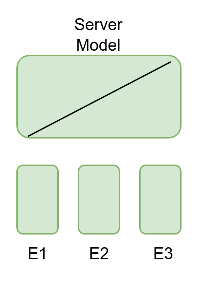
\includegraphics[height=2.7cm,keepaspectratio]{figures/fl_step_1.png} \\
\hline
2 & Distribute the initial model to the clients (devices or local servers). & 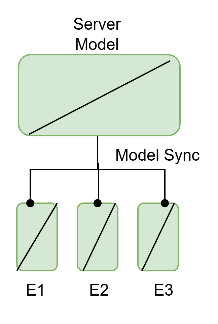
\includegraphics[height=2.7cm,keepaspectratio]{figures/fl_step_2.png} \\
\hline
3 & Every customer keeps training it locally with their own data. & 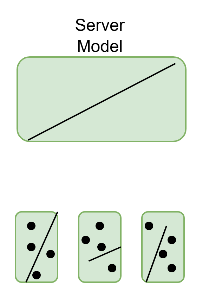
\includegraphics[height=2.7cm,keepaspectratio]{figures/fl_step_3.png} \\
\hline
4 & Through secure, encrypted communication, clients communicate their locally trained model updates to the shared server. Rather than passing on original data, only model parameters---such as the neural network weights---are exchanged. The centralized server subsequently aggregates and averages parameters to optimize the global model's performance. & 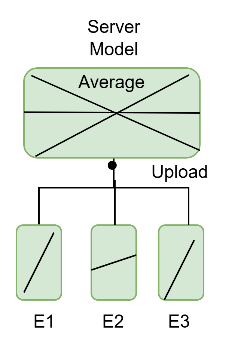
\includegraphics[height=2.7cm,keepaspectratio]{figures/fl_step_4.png} \\
\hline
5 & This trained model is sent to all participating devices and servers. & 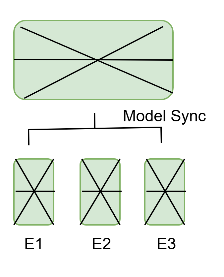
\includegraphics[height=2.7cm,keepaspectratio]{figures/fl_step_5.png} \\
\hline
\end{longtable}
\setlength{\tabcolsep}{6pt}

\subsection{Federated Learning and Personalized Recommendation System}
The decentralized ML technique known as Federated Learning (FL) allows edge devices to collaborate with a centralized server located anywhere in the world to construct a global model. While communicating with the server, these edge devices use trained parameters or gradients to keep sensitive data private.

With the support of a global server, FL enables edge devices to develop a global model in a decentralized ML approach. While communicating with the server, these edge devices use trained parameters or gradients to keep sensitive data private. In FL, a global server and other devices called local clients work as edge devices. It enables learning at edge devices, which involves training models on data distributed across thousands of devices. At the same time, it lets you improve results in both the peripheral and the central systems.

The application domain in which FL demonstrates significant advances over traditional ML solutions is Recommendation Systems. FL-based recommendation systems can learn faster and provide better recommendations. As the data remains confined to the user's environment, this innovative method allows models to be trained on devices without compromising user privacy~\cite{ref9}.

This requirement turns into the challenge of fitting large and complex neural networks on edge devices. Different approaches like Self-Governing Neural Networks (SGNN), SGNN+, and Projected Attention Network (PRADO) have been studied, which work with limited memory and computational capacity. Among these three methods, PRADO has been found to perform better for NLP applications.

\subsubsection{Transfer Learning}
Transfer learning is crucial in ML when only limited data is available for a specific problem. Usually, huge amounts of data are available for general categories, making it one of the first methods used to address cold-start users in recommendation systems and machine learning. For example, training a model to identify a specific product and other labels on a store shelf can be challenging if there are not many training photos of the specific products available. For a general domain like image training, one has sufficient training data, e.g., the ImageNet dataset. Transfer learning employs such a dataset in order to succeed in overcoming the problem of accommodating a model with a limited dataset~\cite{ref11}.

Federated Learning (FL) is closely related to Transfer Learning (TL) in the sphere of ML. TL provides a useful mechanism for utilizing pre-trained deep learning models that researchers have trained using large computational resources and a wide range of data for more specific tasks. This approach allows researchers to take tested models and apply them to concrete issues, improving efficiency and effectiveness in various applications. Building on this concept, Federated Learning, as well as Transfer Learning, are merged together to form Federated Transfer Learning (FTL). FTL is an advanced approach that ensures that FL techniques are used in various local datasets to collaboratively learn a common portion of the model architecture. This knowledge can be applied for certain tasks in each field. To illustrate, both a sentiment analysis model and a text summarization model may use a shared sentence-encoding component, which is trained through FL, making them more efficient and allowing them to perform the same tasks progressively better. The main ideas behind gaining training efficiency and iterative refining in the FL paradigm are TL and its extension, FTL~\cite{ref12}.

\subsubsection{Personalization}
According to~\cite{ref13}, personalization is a new area of research in federated learning, whereby the model learns using local data in individual devices, which leads to personalized enhancement with privacy. The raw data remains decentralized and never leaves users' devices. Personalization in federated learning occurs through updating the model parameters stored locally on users' devices or servers. These updates are typically based on each user's interactions, behaviors, or preferences. For example, in a federated learning system for a mobile keyboard app, the model may learn from each user's typing habits, frequently used words, or language preferences without sharing keystrokes or text input~\cite{ref13}.

\subsection{Categorization of Recommender Systems in FL Environment}
Federated recommendations are classified according to the recommendation system's data structure, which primarily involves two entities: users and items. Shared users or items arise from a natural connection between the parties in a Federated Recommendation. Two major types of these systems are: architecture-based and those organized by user and item features, known as Horizontal, Vertical, and Transfer federated recommendation systems~\cite{ref12}.

\subsubsection{Architecture-based}
The architecture employed for federated learning determines the form that recommendation systems can take: centralized, hierarchical, regional, or decentralized. In a federated recommendation system, all edge nodes connect to a central aggregation node, allowing local weights to be updated and models to be distributed. This setup is shown in Figure~\ref{fig:arch}. By installing numerous coordinators or regional aggregation nodes, data exchange can be reduced, and control over local devices can be increased. A more streamlined technique would be to move the aggregating function to the edge. When a global or regional server experiences heavy traffic and becomes a bottleneck, this setup serves as a viable backup plan~\cite{ref12}.

\begin{figure}[H]
\centering
\begin{minipage}[c]{0.45\textwidth}
  \centering
  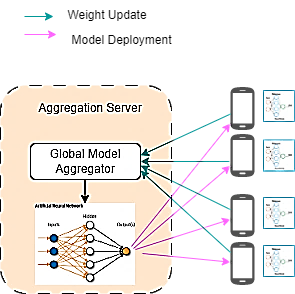
\includegraphics[width=\linewidth]{figures/image9}
  \smallskip\\
  {\small (a) Centralized}
\end{minipage}
\par\medskip
\begin{minipage}[c]{0.40\textwidth}
  \centering
  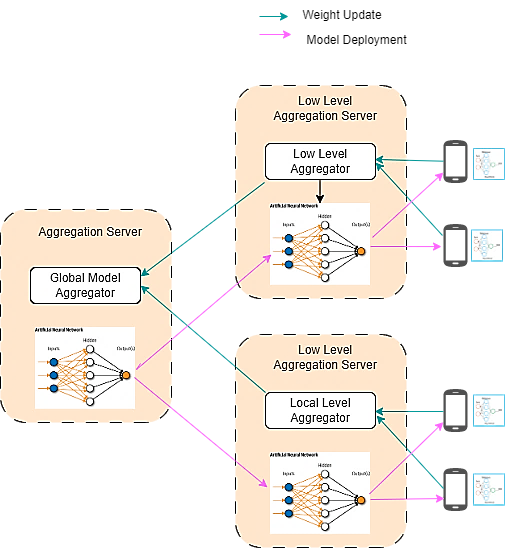
\includegraphics[width=\linewidth]{figures/image10}
  \smallskip\\
  {\small (b) Hierarchical}
\end{minipage}\hfill
\begin{minipage}[c]{0.50\textwidth}
  \centering
  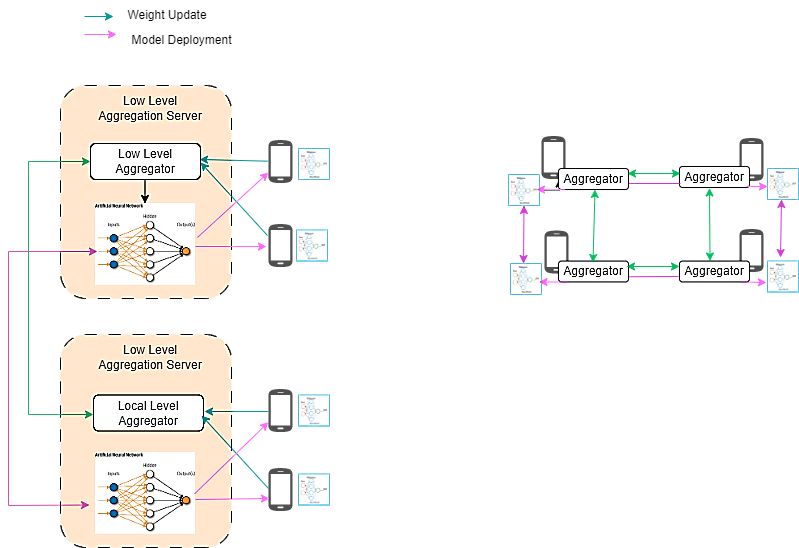
\includegraphics[width=\linewidth]{figures/image11}
  \smallskip\\
  {\small (c) Regional \hspace{1.2em} (d) Decentralized}
\end{minipage}
\caption{Communication architecture for federated recommendation: (a) Centralized, (b) Hierarchical, (c) Regional, (d) Decentralized}
\label{fig:arch}
\end{figure}

\subsubsection{Based on the distribution of Users and Item Features}
\noindent\textbf{Horizontal FedRec:} In horizontal FedRec, items are shared between parties, but not users. The parties can be individual users or groups of users. Several recent studies focus on such scenarios. Matrix factorization served as the basis for a collaborative filtering technique (FCF) proposed in~\cite{ref10}. In conventional recommendation systems, matrix factorization methods decompose the ``user-item'' rating matrix into a product of user and the item latent factor matrix. This method stores user-specific latent features locally on each device, while FCF's collective item latent features are managed by a global server. The server allots item latent factors to all devices involved in the training process at each iteration. After that, they use rating data to fine-tune their users' latent characteristics, then update the server to aggregate everything.

During the training process, no personal user data is gathered; only model updates are communicated. There is no longer any requirement for a central server thanks to the introduction of a completely distributed matrix factorization algorithm in~\cite{ref14}. Direct communication between the parties enhances the model. Furthermore, an alternate decentralized method for matrix factorization was suggested in~\cite{ref15}, in which community members, rather than outside parties, contribute local models. The algorithm's performance is considerably improved by this way.

\noindent\textbf{Vertical FedRec:} In this scenario, two entities share the same group of clients but possess different sets of items or feature spaces. These entities could be different data providers or recommenders. Many researches have been conducted to tackle the challenge of distributed learning when parties possess different features. An asynchronous stochastic gradient descent algorithm was proposed in~\cite{ref16}. To make a local prediction based on its own characteristics, either side can use any model it chooses.

Each side's training can go at their own pace within a given time frame. Reduced privacy issues are a result of this method's omission of raw data and local models. Seamlessly incorporating differential privacy greatly enhances privacy. Groups participating in vertical FedRec can have two recommenders who use different item sets. A book recommendation system and a movie recommendation system, for instance, both serve a large user base but provide distinct content. The goal is to improve recommendation algorithms using secure, privacy-preserving methods. A protected, item-based collaborative filtering method was proposed in~\cite{ref17}.

This approach enhances the effectiveness of multiple recommendation systems, each of which shows different item subsets to the same core group of users. Predicted ratings and item rankings can be calculated while maintaining both privacy and prediction accuracy.

\noindent\textbf{Transfer FedRec:} A transfer federated recommender system is characterized by the absence of shared users or items among participating parties. Typically, the involved entities are different recommender systems. A common example in Transfer FedRec is when a well-known book recommendation system collaborates with a newly launched movie recommendation system to jointly build a movie recommender system. Within this scenario, the users and items from each party are distinct. Building a federated recommender system from scratch is challenging due to the diverse range of users and items used by different organizations. To overcome these limitations, federated transfer learning~\cite{ref18} provides a useful alternative.

A few shared co-occurrence samples act as intermediaries for transferring information between domains. First, each side trains its neural network models using local data. They then work jointly to minimize the loss associated with the co-occurrence samples. Developing a secure and effective client algorithm depends on the secret sharing approach. Another scenario where this method can be useful is when items or users co-occur in the transfer FedRec setting.

\section{Research Gap}
After reviewing the literature, several gaps were identified, which motivated this research work.

\begin{enumerate}
\item The use of federated learning for cross-domain recommendation does not have a real-time implementation. How can we create and develop a federated learning framework?

\item Model training occurs on the edge device in FL, but these devices are resource-constrained, meaning they have limited computational power, memory, and more. How can these constraints be addressed?

\item How can the reviewed information be used to guide the selection of an appropriate case study for evaluating the proposed model?

\item Is the Projected Attention network suitable for improving the performance of edge devices in a Federated Learning environment?

\item Does the above technique help the model learn across domains more efficiently?
\end{enumerate}

\section{Problem Definition}
Consider a scenario where a centralized server and $M$ local clients are involved in the training process. The clients signify individual users, denoted by the set $U = \{u_1, u_2, \ldots, u_m\}$. For each user $u_i$, an emotion embedding vector $e \in \mathbb{R}^{d}$ is extracted from their reviews, forming the set of user emotions $E = \{e_1, e_2, \ldots, e_m\}$. Let $T = \{t_1, t_2, \ldots, t_n\}$ be the set of target domains, and let $V = \{v_1, v_2, \ldots, v_n\}$ denote the corresponding set of review texts associated with each item. The primary goal is to predict the appropriate emotion vector $e_i$ for each user and recommend the most relevant target item $t_j \in T$ whose reviews semantically match the user's emotional profile.

\section{Objectives of the Proposed Research}
The objective of the research is ``Designing a real-time modular federated learning system for cross-domain recommendation''.

\begin{enumerate}
\item Design and develop a scalable and modular federated framework.
\item Integrate a Projected Attention Network into a Federated Learning framework to predict emotions.
\item Develop a new federated Cross Domain Recommendation (CDR) system that uses federated transfer learning.
\item To assess the outcome of a federated CDR in comparison to baseline models.
\end{enumerate}

\section{Contribution of the Thesis}
The important contributions of the research work are:

\begin{enumerate}
\item The first contribution is the development of a federated learning framework designed to protect user data privacy. The developed framework is integrated with the Projected Attention Network to predict emotions. This process includes three modules: a projection layer to extract important features from the review text, an attention layer to capture these features, and a convolutional layer with SoftMax for classification.

\item Federated cross-domain recommendation is the second contribution, in which emotions serve as the source domain and Book, Movies, Music, and Game as the target domain. This employs a transfer learning technique in a federated environment. These techniques include aggregating weights for emotion prediction across different clients using a weighted FedAvg algorithm on the central server and an enhanced random forest classifier.

\item The modular FedCDR approach is proposed and compared in two segments: first, the model is evaluated for emotion prediction with baseline models, namely LSTM, Bi-LSTM, BERT, and PRADO; and second, it is evaluated across domains with the help of EMCDR, CDFLM, and ANR. As the third contribution, it is also compared with SOTA models like FL-EMCDR, FL-CDFLM, FL-ANR, and MFPCDR.
\end{enumerate}

\section{Organization of Thesis}
Chapter~1 introduced recommendation systems and emphasized the significance of federated learning for personalized recommendations. It also explained how federated recommendation systems are classified.

Chapter~2 reviews different studies on recommendation techniques and federated recommendation systems. It also covers the federated cross-domain recommendation system and describes the research objectives.

Chapter~3 expands the concept of emotion-driven sentiment analysis with a federated learning framework, which is part of the further research work to demonstrate cross-domain recommendations based on user emotion.

Chapter~4 details the new multi-objective Federated cross-domain recommendation that uses a PRADO.

Chapter~5 presents the findings of the proposed model and compares them with state-of-the-art systems.

Chapter~6 offers concluding remarks on the research conducted and deliberates future scope.

\chapter{Literature Survey and Methodology}
Established recommendation systems face numerous security threats, plus privacy invasions and data breaches. Their distributed architecture involves multiple parties and data sources, increasing the risk of privacy violations. These security issues are extremely serious; any privacy violation may undermine user trust and dent the platform's or enterprise's reputation. Users who feel that their privacy has been violated are likely to be hesitant to give personal information or even interact with the recommendation system. This means the information will not be available and user satisfaction will be low. Besides, breaches of privacy can put the platform or business in danger of legal and regulatory action, such as fines and lawsuits \cite{ref19}.

\section{Brief Overview of Recent Literature}
\subsection*{Overview of FL-based Recommendation Systems}
To address privacy risks, Google launched federated learning in 2016 \cite{ref20}. Using this paradigm, the recommendation model can tap into a very large corpus of data from different sources, regardless of location or device type. The distributed architecture allows the model to use a more heterogeneous dataset during training by avoiding dependency on a single server. The ability of federated recommendation systems to combine the ideas of many users enables them to better understand users' interests, habits, and activity patterns, which can subsequently enable them to make more diverse and accurate recommendations. The research focuses on recommendation systems in a Federated Learning environment. The literature review comprises of topics such as cross-domain recommendation (CDR) systems, advanced methodologies, security challenges, traditional federated learning--based recommendation techniques, and federated cross-domain recommendation systems, as revealed in Fig. 2.1. To demonstrate the proposed approach, an emotional intelligence--based case study on book recommendations is presented, in which Movies, Song(Music), Books, and Games are the goal domain, and emotions are the source domain. Additionally, the review explores emotion prediction within a Federated Learning setting. The recommendation techniques are overviewed in this section.

\subsection{Conventional Approach to FL Recommendation System}
In a time of information overload, recommender systems are useful in helping users with relevant and well-targeted suggestions. This is vital in improving search results and the overall quality of the recommendation. At the same time, the privacy and security of user data should be ensured.

\begin{figure}[H]
  \centering
  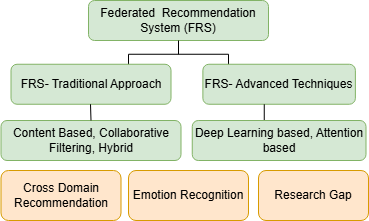
\includegraphics[width=0.8\textwidth]{figures/image12}
  \caption{Figure 2.1 Literature Review Organization}
  \label{fig:ch2_f1}
\end{figure}

Therefore, Ben Tan et al. developed FedRecSys, which supports various online applications, such as item recommendations, content, and online ads \cite{ref20}. The procedure and its employment are available under a free license. This work presents a Federated Recommender System (FedRecSys) designed to tackle security and privacy issues in online recommendation platforms. FedRecSys leverages a federated learning system in which several parties collaborate to train models while keeping user data decentralized on local devices. When deployed in real-world scenarios and integrated with many leading recommendation algorithms, the system shows improved click-through rates (+11\%) and longer average reading times (+22\%). Real implementations have proven successful in content recommendation applications.

To enhance the recommendation system’s accuracy, Su and Guanyi proposed a federated online learning model to encourage knowledge sharing. For mobile social networks, they unveiled a recommendation algorithm. To encourage customers to take part in model training, which would increase both their and the third party's (TTP) utilities, they devised a contract-based incentive structure \cite{ref21} .

FedSPLIT, an implementation of federated collaborative filtering (CF) that does not require supervision and employs NMF joint factorization \cite{ref22}. To generate one-of-a-kind recommenders, first, clients execute local CF concurrently. The next step is to tell the processor to use joint factorization to retrieve global item patterns while protecting each client's local items' privacy by analyzing them for patterns and biases. This is followed by pattern aggregation via knowledge distillation, and then the results are shifted to each participant to modify their local models.

The writers discussed concerns about the impact of recommendation algorithms on users' privacy. It is possible to make suggestions without divulging private information. They introduced an algorithm for federated recommendations, FedeRank (https://split.to/federank). Different devices use different factorization models. To train this model, the central server and federated clients operate in tandem. Users have discretion over the amount of information they share and FedeRank conducts recommendation computations in a distributed manner. Extensive experiments demonstrate that, in comparison to SOTA algorithms, FedeRank achieves higher accuracy with very little user data sharing \cite{ref23}.

Ensuring fairness, or uniformity, in the performance of recommendations among federated learning participants is the main topic of the article by G. Lin et al. Their suggested framework, Cali3F, connects the neighborhood to a federated CF recommendation system in order to do this. Training both local and global models is achieved through a multitask learning framework. FedRec is a federated learning-based recommendation system designed to protect privacy while predicting customer ratings. Although traditional collaborative filtering methods risk exposing user preferences, FedRec addresses this by keeping rating activities private. The framework introduces two main approaches: hybrid filling (HF), which replaces unrated items with projected ratings based on negative feedback; and user averaging (UA), which provides an average rating for unrated items. FedRec reduces privacy risks and computational costs while maintaining accuracy comparable to non-federated models, based on tests using the MovieLens 100K and 1M datasets. The work highlights FedRec's versatility and its relevance to models such as SVD++, beyond Probabilistic Matrix Factorization (PMF). As a result, both computational speed and fairness are improved \cite{ref24}.

The study by Liang F et al. looked at privacy-aware suggestions with direct comments. The authors present FedRec++, an innovative lossless FRS that leverages filtering clients to remove noise generated by virtual ratings assigned to a random sample of items. Furthermore, the authors examined FedRec++'s privacy features and revealed that it provides robust privacy to users\cite{ref25} .

The researchers provide detailed explanations of numerous methods and advancements in this area. In their chapter, Yang, L. Tan, B., and others describe federated recommendation systems in great detail. The horizontal, vertical, and transfer learning are the pillars of federated learning---form the basis of this summary. User-item sharing scenarios determine the classification (feature space). The difficulties of developing federated recommender systems are discussed. Additionally, federated recommendation systems are categorized at both the algorithm and system levels \cite{ref12}.

Both stakeholders and recommender systems benefited from the use of FL by Saikishore Kalloori et al. To form a federated recommendation model cooperatively using training data from the client's or other stakeholders' systems, they devised a federated learning approach that averages model updates. Two widely used algorithms, including Neural Collaborative Filtering and Bayesian Personalized Ranking, were used to implement this strategy \cite{ref26}.

The initial federated Collaborative Filter implementation was presented by Muhammad Ammad-ud Din et al., and it updates models using a stochastic gradient method. A classic machine learning case study is presented in the paper, which analyzes a customized recommender system that relies on implicit user input. Due to its simulation nature, the system requires further investigation into the actual case of clients' asynchronous data transfer \cite{ref9}.

The authors examined the key challenges and recent advancements in federated recommendation systems in \cite{ref28}.

\subsection{Enhanced Techniques for FL Recommendation Models}
In an attempt to use user-item interaction to generate new insights using additional information of the user , Wang Q. et al. \cite{ref13} designed PrivRec, a deep neural network-based recommendation engine to deal with the issue of the asynchronous nature of data transmission. They proposed a successful, practical meta-learning approach for PrivRec that enables FL to support data heterogeneity and idle users in recommender systems. In addition, they enhanced the privacy of PrivRec by introducing user-level differential privacy features, which reduced the likelihood of revealing sensitive information to malicious FL clients. In turn, DP-PrivRec became a more resilient and secure model.

To protect sensitive information without affecting the training process or the model's performance, Liu Yang et al. proposed a tailored masking strategy to mitigate the computational overhead of DP-based systems. By applying it to the FedMMF algorithm, they have proven that this method is effective in the recommendation scenario. In addition, FedMMF demonstrates better performance, both in theory and in practice, by using an adaptive secure aggregation algorithm. \cite{ref30}

Continuing in the same way, Amir J. et al. have presented an FL strategy for recommender systems that is both simple and effective in improving customization. Related meta-learning algorithms are also discussed. The outlined method outperforms the existing FL recommenders in real-world scenarios while being simpler to implement. The authors tested the algorithms' ability to forecast user ratings using benchmark data and evaluated their performance experimentally using RMSE. Encryption is necessary to guarantee the user's anonymity when reconstructing their gradients or parameter modifications. \cite{ref31}

For session-based RNN modeling, Yang, L. et al. have proposed multiple parallel RNN architectures that incorporate click data and attributes, such as linked images and text. They went a step further by suggesting improved training methods for P-RNNs beyond the current standard. The results demonstrate that compared to featureless session models, p-RNN architectures perform significantly better when trained correctly. By comparison, session-based models yield better results than the item-wise average.\cite{ref32}

This research introduces a Privacy-Preserved Recommender System Framework (PPRSF) designed to manage the privacy-personalization trade-off in traditional recommender systems based on Federated Learning (FL). By separating public and private user data, PPRSF reduces privacy risks while maintaining recommendation quality, enabling model training without centralized data collection. The framework features a four-layer hierarchical structure: the Recall Layer (server-side) pre-filters candidate items; the Ranking Layer (client-side) refines recommendations with private data; the Re-Rank Layer (server-side) enhances diversity and fairness; and the Service Layer (client-side) presents results and collects new interactions. FedAvg facilitates the pooling of locally trained ranking algorithms across the globe.

A privacy-protecting FL method for top-N POI (points of interest) ideas, FedPOIRec, that uses users' social network data was introduced by Perifanis, Vasileios, Drosatos, et al. to raise awareness of the technology. The FedPOIRec architecture states that clients retain local data and updates while the server aggregates them. By letting users share learned parameters, FveriedPOIRec also facilitates knowledge exchange among friends. \cite{ref32}

Combining social impact with data privacy, FedPOIRec is an FL system developed to preserve privacy in POI recommendations. Secure Multiparty Computation (SMC) and Fully Homomorphic Encryption (FHE) are used for secure model aggregation and social feature integration, unlike traditional centralized models that store user data on local devices. FHE has significant processing costs, and the system encounters issues with sparse data and cold-start users. Other unresolved challenges include adversarial robustness and scalability on devices with limited resources \cite{ref32} \cite{ref34}.

\subsection{Safeguarding Federated Recommendation Systems}
The researchers integrate user preferences for federated computation with a program that protects privacy and leverages all features of the CKKS homomorphic encryption system \cite{ref34}. With the FGBDT system, MNOs and HPs can engage in collaborative modeling while protecting users' privacy without compromising data exchange. Better user classification using combined MNO and HP data is a potential outcome of using the suggested system in healthcare recommendation apps \cite{ref35}.

I. Guillén et al. discussed a privacy-preserving recommender system (RS) using Federated Learning (FL) to address growing ethical and legal concerns about collecting user data. Unlike other centralized RS models, the proposed method stores raw user data locally, preserving both recommendation accuracy and privacy. Instead of directly merging synthetic user profiles, the system generates them through a consensus-based aggregation process, thereby avoiding privacy issues by retraining models rather than merging them directly. The system was tested with GreenSoul and Prolific datasets (N=678) and evaluated using the Normalized Distance-Based Performance Measure (NDPM), employing four Raspberry Pi devices and an NVIDIA Jetson Nano as the aggregation server. Results indicate that, even with reduced communication and processing costs, the FL-based RS delivers accuracy comparable to or better than centralized approaches. Additional privacy protections are provided by a hybrid encryption system that secures model updates \cite{ref2}.

Based on matrix factorization, J. Zhang and Y. Jiang \cite{ref35} presented a hybrid, clustered, vertical, federated matrix recommendation method. They modify the prediction score of the federated matrix factorization recommendation model by adding a user-clustering strategy. This approach makes it easier to cluster users' latent factor vectors. This approach guarantees that user rating information remains within each recommendation system while enabling the proper study of user-item correlations. Using homomorphic encryption, consumers' private data is protected. M. Dogra et al. introduce a novel approach to Recommender Systems (RS) built on Federated Learning (FL). The items and users in this method are encoded in a fixed-size format that remains constant regardless of their quantity. This method works well for large-scale RS applications and uses little memory. Using a Next App Recommendation use case, the framework has been proven to deliver performance on par with previous solutions while consuming much less memory\cite{ref36}.

\subsection{Cross Domain Recommender Systems}
CDR methods can be categorized by their focus on content, features, embedded transformation, ratings, or a mix of these. To integrate attention mechanisms at the item and domain levels, the authors proposed a neural network method called NATR.  To protect privacy, the Neural Attentive Transfer Recommendation (NATR) model employs attention mechanisms at the item and domain levels to extract proper collaborative filtering (CF) signals from transported embeddings. Evaluated with MovieLens-Netflix and iQiyi-Tencent Video datasets, NATR outperforms traditional cross-domain models (CMF, ItemCST), achieving up to 18.94\% higher HR@10 and resolving cold-start problems for items. However, the research has limitations, including embedding dimensionality inconsistencies, scalability issues in large-scale environments, cold-start user problems, and security vulnerabilities to adversarial attacks. Transferring item embeddings from the secondary domain helps address issues in CDR learning by preventing user privacy leakage. No research has been conducted on the approach's scalability  \cite{ref37}.

To create user and object latent factors, the researchers in  \cite{ref38} presented a matrix factorization-based approach that subsequently employs deep neural networks to map these factors across domains. This paper proposes a deep learning module for CDR, CSR, and CDCSR. It maps user and item latent variables across domains using a DNN and MF, then generates them. It includes benchmarking aspects that account for rating sparsity to ensure a more accurate mapping.   When measuring MAE and RMSE, the model outperforms SOTA techniques on the Douban, Netflix, and MovieLens datasets.   The approach ignores real-time deployment, assumes a fixed mapping function that would not be appropriate across somewhat distinct domains, and omits emotion-based features.   Training the DNN also incurs computational expenses that affect scalability; the model does not fix the cold-start problem for new users or objects.

Other CDRs are working on dual targets. \cite{ref39}, \cite{ref40}  \& \cite{ref41}  . Unlike conventional single-target CDR systems, the DTCDR framework.\cite{ref39} It is a new Dual-Target Cross-Domain Recommendation (CDR) system that improves recommendation accuracy across both domains. It uses Multi-Task Learning (MTL) to distribute user embeddings among domains, hence improving suggestions in both richer and sparser environments. Three embedding combination techniques---concatenation, average pooling, and max-pooling---are investigated to improve information transmission.

The system produces document embeddings (Doc2Vec) and rating embeddings (NeuMF and DMF), and combines data from several sources, including user profiles, ratings, reviews, item data, and tags. With up to 13.73\% improvement in HR@10 and 18.83\% in NDCG@10, experiments on MovieLens and Douban datasets reveal that DTCDR performs better than single and cross-domain models. Still, specific difficulties exist. The computational complexity of MTL-based embedding sharing raises scalability concerns and makes large-scale installations difficult. Cold-start users---who could benefit from meta-learning---are not explicitly addressed by the approach. Furthermore, no adaptive process is proposed to select the optimal embedding combination.

\subsection{Federated Approach to Cross-Domain Recommendations}
The research goals in \cite{ref42}, \cite{ref43}, \cite{ref44}, \cite{ref45},\cite{ref46}, \cite{ref47}, \cite{ref48} , and \cite{ref8} are to address data privacy and the problem of cold-start users in recommendations. They accomplish this by enhancing recommendations using a domain with rich information. The confidentiality of user information is preserved throughout the process of resolving these issues. To guarantee privacy in CDR, the authors presented a Federated framework. The suggested techniques acquire user and item embeddings by training a standard recommender model on all client devic42es. After that, each client sends its weights to the central server. Local differential privacy is a privacy protection scheme that can protect user information by perturbing the weights before uploading gradients. The similarity between a user's embeddings in the two domains is further narrowed by performing embedding transformations at the server. The methods are a privacy-saving and consistent CDR technique with valuable results in privacy assurance and personalized suggestions. FedCDR, which is specifically built around federated learning, places more importance on privacy, but it deals with the problem of sparse data and cold-start users or items in cross-domain recommendation models. FedCDR also allows recommendation-model training to be performed on the user's device, compared to traditional CDR models that use a centralized data warehouse, which helps avoid exposing raw data to unauthorized access. It addresses privacy breaches by adding noise to gradients before sending them to the central server and uses Local Differential Privacy (LDP). In addition, the federated aggregation system, FedAvg, guarantees that raw data are never sent but only encrypted model updates are. Experiments on Douban datasets demonstrate that FedCDR is more efficient than current privacy-saving methods, such as CCMF, and is equally efficient in terms of recommendation quality as centralized models. FedCDR with an appropriate distribution of privacy budget ($\epsilon$), gradient clipping ($\delta$) and noise magnitude ($\lambda$) displays stability under different percentages of cold-start users, thus attaining the ideal privacy-accuracy trade-off \cite{ref42}

The paper presents a Federated Cross-Domain Social Recommendation (FCSR) algorithm, which enables the privacy-sensitive cooperation between social service platforms (SSPs) that store the information in social networks and information-oriented websites (IOWs) that store the information on feedback on users. Conventional cross-domain advice relies on data gathered centrally, thus increasing privacy-related issues, and in most cases, this can be very impractical because of limitations to accessing the data. The authors leverage Federated Learning and use two major privacy mechanisms: the Random Response Mechanism (RRM), which attenuates the perturbation of social contacts, and the Matrix Confusion Method, which encrypts user feature vectors to enable updating features without revealing individual information. The system enhances computational efficiency by decomposing sparse matrices using lower-upper (LU) decomposition, which eliminates the complexity in solving large-scale linear systems. Experiments with FilmTrust, CiaoDVD and Epinions show that FCSR is significantly more accurate than incumbent federated recommendation systems (FedMF, FedGNN, FeSoG) and keeps users private  \cite{ref44}.

CDR is one way to address the cold-start user or item issue in conventional recommender systems. This approach uses exchanges between the source and target domains that allow cold-start users to see personalized suggestions. As much as the present CDR techniques are popular, they rely on a shared-preference bridge, where they share data with each user, thus not capturing the unique and diverse preferences of each user \cite{ref50}.  Moreover, they need direct two-way data exchange between servers and clients, which increases privacy concerns. To overcome such difficulties, the authors proposed a user-specific cross-domain preference bridge based on federated meta-learning. They used FL to train a preference bridge that sums local stored data and model parameters. This plan does not compromise the privacy of users and improves the effectiveness of CDR \cite{ref45}.

IoT innovations boost the rapid increase in large volumes of data. From such large datasets, a cross-domain recommendation engine is effective in determining objects that a user likes. Nevertheless, three issues can be encountered when implementing a cross-domain recommendation system across dispersed IoT devices. Embeddings of currently popular items tend to have a popularity bias. Also, most existing techniques rely on shared-interest channels to convey user preferences. People have different tastes, and thus it is reasonable to expect different users and interests. The information received from dispersed IoT devices can also pose a privacy risk. This paper presents FedBP, a federated FedCDR that integrates a bias eliminator and a custom extractor system to improve recommendation accuracy in cold-start situations. All embedding directions are elongated during training with the help of a bias eliminator, and each route registers only specific information and is neutral in terms of popularity. In addition, a tailored extractor will match users' individual preferences in the domains. This system is trained in a federated architecture and secures data privacy using local differential privacy.\cite{ref46}

The paper in \cite{ref47} introduces a new multi-view federated learning framework, Fed-FR-MVD, developed for data-diverse, privacy-conscious e-commerce environments to increase recommendation accuracy. Current federated learning (FL) methods have issues related to data heterogeneity, inefficient feature extraction, and noise sensitivity, whereas concerns related to data privacy have long plagued traditional centralized recommendation systems. To address these issues, Fed-FR-MVD integrates an item- and user-view-based multi-view architecture that uses a Feature Rescaling (FR) method. FR module is a dynamic feature weighting method that focuses on relevant characteristics and suppresses noise. On the multi-view complex data, a deep structured semantic model (DSSM) can be used to learn a better representation. Experimental findings on Amazon data indicate that Fed-FR-MVD is more robust to noise rates of 5\%-15 \%, and is stronger in comparison to techniques based on single or multiple views by 12\%-18 \% \cite{ref47}.

In \cite{ref48}, an original method of Privacy-preserving Cross-domain Recommendation (PCDR) has been introduced to address privacy leaks in domains and data heterogeneity in federated cross-domain recommendation (FCDR). PFCR uses universal item representations based on text content descriptions, unlike previously presented studies that use user identity overlap to align domains, which puts users at risk of privacy issues. A vector-quantized item representation method uses text to produce discrete codes, which allows efficient semantic matching across domains. Privacy preserving aggregation employs federated averaging (FedAvg) where the gradients of items are shared but user-specific ones remain local \cite{ref48}.

CDR has been used extensively to reduce data sparsity because it cross-domain transfers information. Current studies combine federated learning and CDR due to the potential for compromised data privacy when direct information is exchanged.

However, these methods require homogeneous models across domains and incur significant communication costs, which limit the adoption of federated learning. This paper presents a “one-shot” federated cross-domain ensemble learning system called FedOCD. There are two primary parts to FedOCD: the first is source-domain modeling, which uses source-domain data to learn user embeddings while protecting their privacy via Local Differential Privacy (LDP); the second is the target-domain ensemble, which uses source-domain user features to enhance recommendation performance. FedOCD significantly improves performance, according to experimental results on benchmark datasets. \cite{ref49}

To handle cold-start and data sparsity challenges, CDRs are becoming increasingly crucial for delivering personalized data across disciplines such as e-commerce and healthcare. Accurate recommendations in one area are made possible by using user profiles and adequate ratings in another. Many highly rated places are hesitant to let third-party recommendation systems or domains access user ratings because of privacy concerns. Hence, a privacy framework is required for cross-domain data transfers. To address privacy and cold-start issues in CDR systems, this study presents the CrossRec-Hybrid Federated Transfer Learning (CrossRec-HFTL) platform. It leverages user-item interaction in an annotated source domain to make recommendations in a non-annotated target domain, combining adversarial domain adaptation with federated learning. Simulation findings show that CrossRec-HFTL achieves higher suggestion accuracy than the baseline and modern recommendation systems, with a comparatively low RMSE of 0.82 and MAE of 0.58. This demonstrates the model's improved privacy protection and its great performance in cold-start scenarios \cite{ref8}.

\subsection{Emotion Recognition and Federated Learning}
Researchers in both education and business are always interested in emotion recognition and sentiment analysis. Since federated learning is a relatively new tool, much work remains to be done on emotion recognition. Obtaining multimodal data for emotion detection without sensors and IoT devices is difficult; therefore, text-based emotion recognition has attracted significant attention from researchers in both academia and industry.Audio (e.g., voice emotion detection), visual (e.g., facial expression recognition), and textual data, collectively called multimodal data, have been the main focus of researchers in the works cited as \cite{ref51} and \cite{ref52}. In a federated setting, Nandi et al. \cite{ref52} established a model, Fed-ReMECS, that classifies real-time emotions from physiological measurements obtained from data streams generated by wearable sensors. V. Tsouvalas et al. used a semi-supervised federated learning approach to create speech-emotion recognition in \cite{ref53}. They proved that the addressed method improved emotion identification by 10.0\%. By combining a FedL strategy with a privacy-preserving CNN-based audiovisual model for emotion recognition, Simic et al. achieved a 2\% improvement in accuracy \cite{ref54}.

\begin{figure}[H]
  \centering
  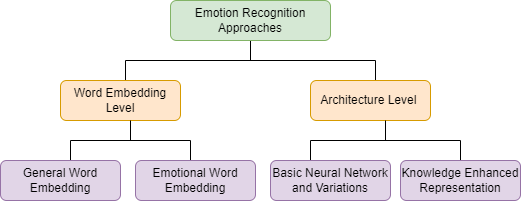
\includegraphics[width=0.8\textwidth]{figures/image13}
  \caption{Figure 2.2 Emotion Recognition Techniques}
  \label{fig:ch2_f2}
\end{figure}

Emotion recognition in text can be achieved in numerous ways. This encompasses several levels of deep learning methods, including training, architectures, and word embeddings, as shown in Figure 2.2  \cite{ref55}.

A mathematical process called ''word embeddings'' can uncover hidden connections between words. Word embeddings are versatile and can be used for both general and emotional purposes. Distributed semantic modeling is the foundation upon which they rest. We have two broad word-embedding models: Word2Vec. \cite{ref56} and Glove \cite{ref57}. According to ELMO \cite{ref58}, Advanced pre-trained models include GPT, BERT, and others alike. Emo2Vec \cite{ref59}, Emoji2Vec \cite{ref60} , and DeepMoji  are examples of models that have already been trained (pre-trained) to process emotional words \cite{ref61}.

Researchers have suggested several neural network models for extracting semantic and sequence information. The use of long short-term memory (LSTM), pre-trained recurrent neural networks (RNNs), gated recurrent units (GRUs), and similar networks is effective. \cite{ref62}.

Many people also use an attention-based approach to speed up training and improve performance. GRU-based attention is used in hierarchical attention. \cite{ref63}, and LSTM is used in TreeLSTM \cite{ref64}. The network collaborative models are composed of several separate models that work together to produce strong, complete models. \cite{ref55}.

For a more thorough understanding, knowledge-enhanced representations take into account prior information, such as language patterns, emotional lexicons, and other commonsense knowledge about emotions. \cite{ref65}. Affective computing includes the study of interrelated attitudes and emotions. Researchers have widely used the FedL method to improve sentiment analysis, data privacy, and isolation.

Ahmad et al. researched aspect-based sentiment analysis (ABSA) \cite{ref66} \cite{ref18}. ABSA pertains to the targeting of sentiment in sentences across various disciplines. This field has made significant advancements due to developments in DL and pre-trained language models. This field is affected by concerns regarding data privacy. The authors proposed a novel approach to address this issue, introducing prompt-enhanced FL (PFL) for aspect-based sentiment analysis (ABSA). This approach combines prompt tweaking and the privacy-preserving aspects of federated learning. The authors introduced PFL-GCN, a graph convolutional network that combines PFL with BERT.\cite{ref67} In FL settings, researchers test solutions to several natural language processing (NLP) problems.\cite{ref68} Han Qin et al. investigated how aspect-based sentiment analysis (ABSA) becomes more complicated due to pattern divergence across sentences from multiple sources. Legal and privacy concerns restrict access to labeled data for all parties, even though it is available across various locations and sources.

Nuria R. et al. investigated Federated Learning in \cite{ref69}, to resolve arguments about annotations in NLP. In sentiment analysis, annotation is vital. During dataset annotation, the suggested approach treats each annotator as a federated client. At last, the model can gather labels from clients worldwide and combine them without human intervention. Discrepancies found among subject-area annotators teach the model new things. Because of its extensive use in research, FedAvg is widely used.

Large language models (LLMs) were adopted in a federated learning (FL) setting by Himkil et. al. \cite{ref70}. FL's privacy characteristics and conformity with legal norms are increasing its appeal for a variety of applications. This research looks at FL in relation to LLMs. The researchers assessed sentiment analysis using BERT, ALBERT, and DistilBERT and discovered that performance is user-dependent. Researchers need to investigate the causes of DistilBERT's increased latency as the number of clients escalates \cite{ref71}.

S. Bansal et al. used topic preference and sentiment analysis to predict personality traits in \cite{ref72}. They used LDA and LSTM models to assess user-generated content from Weibo. Our eight-figure personality forecast. This approach brings up significant privacy concerns and ethical quandaries. The writers demonstrated how to address the highlighted problems effectively. Unfortunately, there was no proof that the FL method was used for privacy control.

Another approach to identifying consumer complaints was suggested by J. Zhao et al. in \cite{ref73}, which uses a graph attention network. As a part of natural language processing, we can categorize social media complaints. This requires a central system of collecting, distributing, and processing data. This solution fails to consider privacy and decentralized data. The authors believed that by integrating a graph-attention network into the federated learning setting, they would be able to solve this issue. The global and local models can be enhanced using adaptive optimization techniques such as the Fedcomb algorithm simultaneously. In terms of complaint recognition, our strategy outperformed baseline techniques. We need to test this model on bigger datasets.

Investigating how Federated Learning (FedL) incorporates sentiment analysis and privacy preservation has been done by Sakhare N.N. et al. \cite{ref74} and Priyam Basu et al.\cite{ref75}. Within the framework of blockchain technology, the authors of \cite{ref74} investigated the spatial FedL approach for sentiment analysis of stock news. It is critical to do in-depth research on each stock before buying. When analyzing stock market fluctuations, it is essential to account for both the short-term and long-term effects of external factors, as well as corporate details. The writers used spatial federated learning (SPL) to retrieve and analyze news stories from the Economic Times' website. Concerns about confidentiality and regional differences were therefore resolved. Federations use a variety of algorithms. In order to make decisions, every federation takes into account public opinion.

The classification of financial text is addressed by FedL in \cite{ref75}. Financial data must be kept private due of its sensitivity. To train large models, this data must be properly managed. The writers used federated learning, differential privacy, and text classification models based on contextualized transfer learning. The model outpaced the SOTA transformer; though, it performs miserably on imbalanced data.

\subsection{Investigations based on review}
The research gaps identified in the traditional approach to federated learning recommendation systems are:  No direct comparison is provided between federated learning-based recommendation models and centralized recommendation models in terms of accuracy, precision, and recall \cite{ref21}, \cite{ref22} \& \cite{ref24}. A few approaches in our discussion are group-based, meaning individual users cannot directly participate without a predefined group  \cite{ref23} \cite{ref25}. Many approaches focus on a single domain \cite{ref22} \cite{ref26} \cite{ref12} \cite{ref27}. The traditional approach does not address Cross-domain recommendation. Recommendation systems are simulation-based; hence, they lose the real-world context \cite{ref27} .

The research gaps identified in advanced techniques for recommendation in Federated Learning include computational overhead concerning the use of advanced ML algorithms \cite{ref30}\cite{ref31}, cold-start issues, scalability constraints\cite{ref32} , and security vulnerabilities to adversarial attacks\cite{ref9}.

The research gaps identified in security for federated recommendation systems are: the use of different encryption techniques results in Computational Overhead and Scalability \cite{ref29}\cite{ref33}\cite{ref36}, and Real-World Deployment Feasibility \cite{ref37}.

The research gaps identified in CDR systems are: The model discussed in \cite{ref39} does not address the cold-start problem for new users or items. While the DNN improves mapping accuracy, training a deep network requires considerable computational resources \cite{ref39}, \cite{ref40}  and \cite{ref41}. All these systems rely on sharing user data across different domains for accurate recommendations \cite{ref39} \cite{ref40}, \cite{ref41} and \cite{ref42}.

The research gaps identified by Federated Cross-domain Recommendation (FedCDR) systems include: communication costs and communication overhead \cite{ref43} \& \cite{ref44} , scalability concerns, scalability challenges, cold start issues \cite{ref45}, and the ongoing challenge of real-world validation \cite{ref46}, \cite{ref47}, \cite{ref48} , \cite{ref49}, \& \cite{ref8}.

Reviewing the literature on Emotion recognition [46-66] shows that no previous implementation has addressed the challenge of deploying neural networks on mobile devices with restricted resources and bandwidth.

\section{Methodology}
The proposed research applies an organized methodology to design, implement, and evaluate a multi-objective cross-domain recommendation system within a federated learning framework.

\subsection{Overall System Design}
The system is structured into three major layers:

\begin{itemize}
    \item Local Client Layer: This layer is responsible for data processing on the local device. The local model is trained, and emotion prediction is done. The PRADO architecture is used for feature extraction and emotion classification on edge devices.
    \item Federated Aggregation Layer: The layer includes the central server, which is responsible for collecting weight parameters and aggregating them with the FedAvg algorithm to build a global model.
    \item Recommendation Layer: This layer performs cross-domain recommendation using federated transfer learning and an advanced recommender using cosine similarity-based fingerprinting.
\end{itemize}

This layered architecture ensures privacy preservation, modularity, and scalability.

\subsection{Data Collection and Processing}
\subsubsection{Data Collection}
This research utilizes two primary datasets:

\begin{itemize}
    \item GoEmotions Dataset: Contains approximately 58,000 Reddit comments, annotated with 27 emotion labels and one neutral category, and used for emotion prediction tasks.
    \item Books Dataset: This is derived from the Kaggle Books\_rating dataset. It contains approximately 10,000 curated book titles and reviews, categorized into fiction and non-fiction genres.
    \item CMU Movie Summary Corpus: 42,306 Wikipedia movie plot summaries and a rich set of movie and character metadata for NLP and recommendation research \cite{ref95}.
    \item Genius Song Lyrics Dataset: A large-scale song lyrics database and metadata set with lyrics from Genius around music, sentiment, and emotion analysis.
    \item Steam Games Dataset: This is a metadata database for more than 83,000 Steam games, comprising their genres, their developers, their release data, their pricing, and their review scores.
\end{itemize}

These datasets enable cross-domain learning by linking user emotions from social media with target domain recommendation preferences.

\subsubsection{Data Processing and Feature Extraction}
Data preprocessing includes convolution and pooling. The Projected Attention Network (PRADO) is used for feature extraction due to its efficiency on resource-constrained devices.

PRADO replaces traditional embedding layers with projection-based representations, reducing memory requirements. The model performs:

\begin{itemize}
    \item Projection-based embedding
    \item Convolutional feature extraction
    \item Attention-based weighting
    \item Text encoding
\end{itemize}

The extracted features are then used for emotion prediction and further integrated into the federated learning pipeline.

\subsection{Local Model Training}
The local model on each client is trained using the Projected Attention Network (PRADO) architecture. It captures important features from the given text input and performs emotion classification locally on each client device.

The Fig. 2.3 demonstrates the overall working of the proposed system.

\begin{figure}[H]
    \centering
    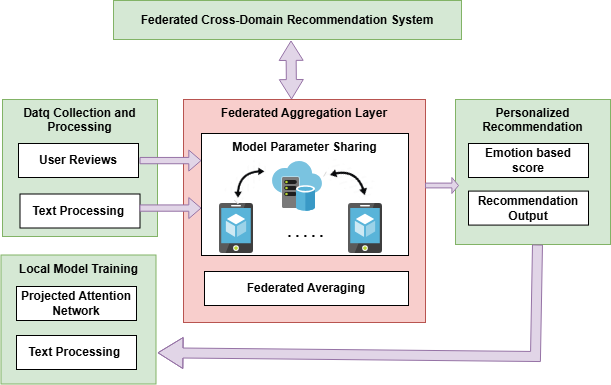
\includegraphics[width=0.8\textwidth]{figures/fig2_3_framework}
    \caption{Federated Learning Framework for Recommendation System}
    \label{fig:fed_framework}
\end{figure}

\subsection{Federated Learning \& Model Aggregation Process}
The process includes an iterative communication protocol as demonstrated in Fig. 2.3. Each client trains the model locally using PRADO. The trained model weights are sent to the central server, where they are aggregated using the FedAvg algorithm to produce an updated global model. This global model is then distributed back to the clients for the next round of training.

\subsection{Personalized Recommendation}
The aggregated global knowledge is received, which includes updated local model parameters for emotion prediction. Based on these parameters, the recommendation module generates personalized recommendations for each user across different domains using cosine similarity-based fingerprinting and random forest-based lookup.

\section{Summary}
This chapter reviews various recommendation approaches within a federated learning environment. It covers traditional methods, advanced techniques for federated recommendation systems, security concerns, CDR systems, and federated CDR systems. Each system mentioned is discussed in detail. The chapter identifies research gaps in accuracy, cold-start issues, scalability, security, and real-world deployment that motivate the proposed system.


\chapter{Emotion Driven Sentiment Analysis Framework for Edge Devices}
Edge devices can manage the large volumes of unstructured data generated by continuous connectivity. Analyzing this data to understand people's actions has boosted the popularity of emotion detection and sentiment analysis. The most common way people express their feelings is through written text. Emotion recognition can be automated using natural language processing. Recent developments in attention-based approaches and deep learning (DL) have strengthened support for research in this area. \cite{ref55}.

\section{Emotion Recognition}
Comments, posts, and reviews on social media platforms like Instagram, Reddit, Facebook, and Twitter help us infer users' emotional states, such as happiness, appreciation, enthusiasm, pride, rage, fear, anxiety, sadness, and curiosity. Emotion recognition is the detailed analysis of human emotions. Despite the frequent interchangeability of the terms, sentiment analysis and emotion recognition are actually separate concepts \cite{ref28} .

Emotional or psychological states include a broad spectrum of mental conditions, such as joy, enthusiasm, grief, and bewilderment. One application of emotion recognition is the examination of mental health records to identify potential offenders \cite{ref51}, \cite{ref52}. Natural language processing applications that leverage DL require data centers and specialized hardware. However, issues like data isolation, user privacy, and high operational costs hinder NLP development. Because traditional ML algorithms rely on centralized data for training, they face challenges in meeting General Data Protection Rule (GDPR) requirements and building user trust. FL is a decentralized approach that complies with GDPR and enhances data protection and privacy. This emerging method for emotion-driven sentiment analysis in a federated environment helps ensure privacy and improve performance.

\section{Strategic Approach to Framework Development}
Traditional text classification methods rely on high-dimensional, low-density lexical features, such as n-gram representations, and use linear models, such as Support Vector Machines (SVM) or logistic regression. Numerous neural network and transformer techniques, such as LSTM and CNN, have enhanced the proficiency of ML models. But these techniques focus on model performance without considering the size or memory constraints of edge devices. In \cite{ref76}, authors proposed an on-device neural network model for user privacy. They developed self-governing Neural Network (SGNN) and SGNN+ models. These models were static and could classify short text. In \cite{ref75} , the authors developed the Projected Attention Network (PRADO), a trainable projection network to capture long text with an attention mechanism.

In improving emotion guessing via federated learning, PRADO offers a practical approach to achieve better model performance while protecting user privacy. By leveraging PRADO's efficient and reliable on-device neural network design, the method incorporates collaborative weight operations supported by the FL framework. The collaboration enables effective, client-side model aggregation that is both secure and scalable, enabling real-time processing.

\subsection{Proposed PRADO-based emotion recognition}
The projected attention neural network-based federated learning framework is an innovative concept that integrates the simultaneous federated training of projections, attention processes, and convolutions. Figure 3.1 shows the architecture in more detail. The framework is composed of:

\begin{itemize}
    \item Local transformation module: Several client devices execute the text data within each user model with the help of the PRADO system, but do not share the raw data. A local model is trained, and only the learned parameters are uploaded to a central server.
    \item Server module: A federated averaging model is aggregated from local model updates to obtain a global model. The new parameters are then sent to all of the clients for the subsequent training round.
\end{itemize}

The right-hand side displays the PRADO model's internal structure. The long input text is then converted to short, trainable embeddings (as shown in the lower part of Figure 3.1) and passed through several convolution and attention modules.

\begin{figure}[htbp]
  \centering
  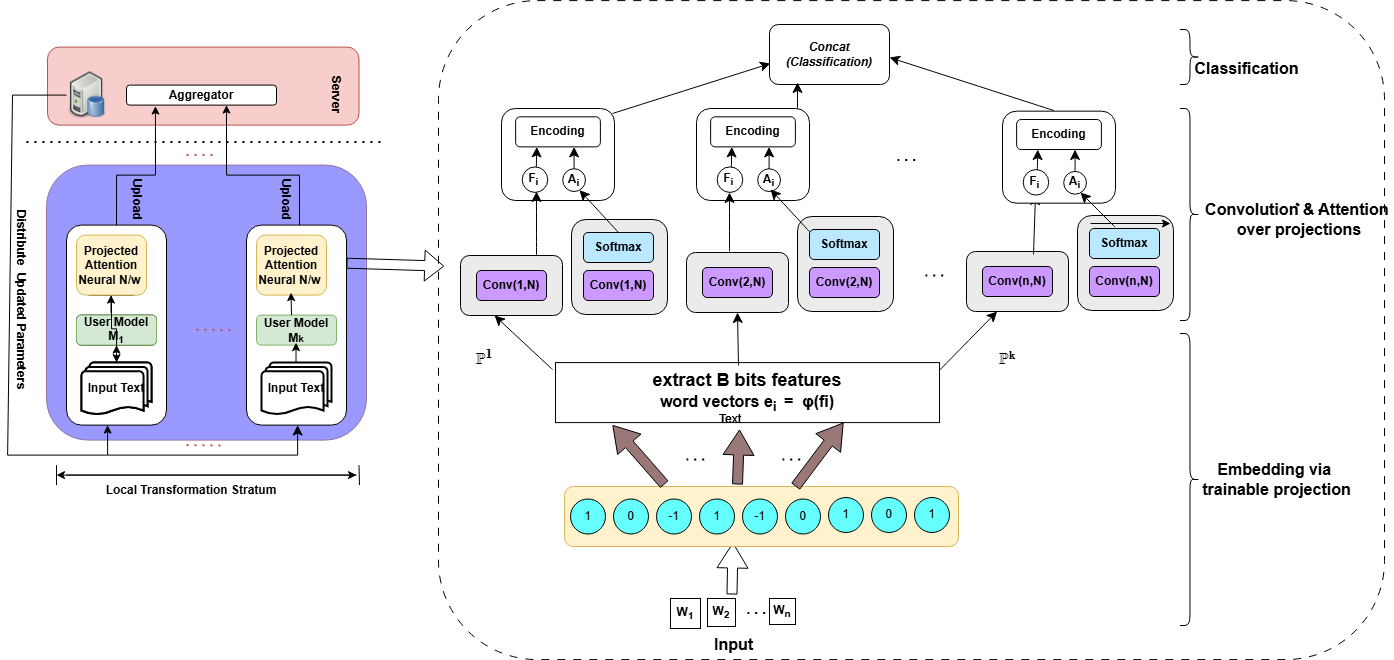
\includegraphics[width=0.8\textwidth]{figures/image15}
  \caption{Federated Learning Framework for Emotion Recognition using PRADO}
  \label{fig:ch3_f1}
\end{figure}

It learns local and contextual semantic properties (middle part of Figure 3.1). The extracted features from various projections are encoded, then combined, and then fed to a classification layer containing a Softmax function for predicting the emotion class (Upper part of Figure 3.1).

\subsection{Working of the PRADO model}
The objective of the PRADO is to classify the emotions using a compact neural network architecture on resource-constrained edge devices. Conventional deep learning models require a large vocabulary and high-dimensional embedding matrices. Using a projection operation, PRADO dynamically generates trainable embeddings. This reduces memory requirements. As discussed earlier, the PRADO model comprises projected embeddings, convolution-based extraction, attention-based feature weighting, and classification. The PRADO process is described using equations (3.2) to (3.8) from \cite{ref75}.

Let an input consist of a sequence of $T$ tokens $\omega_0$, $\omega_1$, $\omega_2$, \ldots, $\omega_{T-1}$. Here $\omega_i$ represents $i$-th token. This token refers to a pre-processed individual word from the input text. The pre-processing may include converting text to lowercase, separating punctuation symbols, and tokenizing the sentence into individual words.

Example: - “I like the rose flowers.” is tokenized as { I, like, the, rose, flowers }. Each token is processed before contextual information is extracted.

In traditional NLP models, each word $\omega_i$ is mapped to a one-hot vector, where $|V|$ is the vocabulary size. It contains a value `1' at the index corresponding to this token and zeros elsewhere. Then, the embedding layer maps to the words,

\begin{equation}
  e_{i} = W \delta_{i}, \quad e_{i} \in \mathbb{R}^{d}
  \label{eq:ch3_3_1}
\end{equation}

\noindent Where $e_{i}$ represents the embedding (or encoded vector) corresponding to the $i$-th token, and it is a $d$-dimensional real-valued vector. $W$ is a weight (or embedding) matrix, typically of size $|V| \times d$, where $|V|$ is the vocabulary size and $d$ is the embedding dimension. $\delta_{i}$ is a one-hot vector of size $|V|$.

This illustration captures semantic information effectively, but the embedding matrix size is proportional to vocabulary size and hence requires large memory storage. This makes the technique unsuitable for edge devices.

\subsubsection{Projected Embedding Layer:}
PRADO addresses this problem by replacing standard embeddings with a projection operation. Each token is transformed into a compact binary fingerprint by applying a hashing function. It generates compact embeddings by hashing each word to a 2B-bit fingerprint. It partitions this into B, 2-bit groups and maps each group to a ternary value in $\{-1, 0, 1\}$. B represents the projection dimension. This results in a projection vector $f_{i}$.

Consider the same example, “I like the rose flowers”. Tokens generated are {I, likes, the, rose, flowers}. Suppose the token “like” is selected. Conventional embedding methods look up the word “like” in a large vocabulary table; instead, PRADO generates a numerical representation via a projection operation.

\subsubsection{Step 1: Generate fingerprint}
The word ''like'' is first run through a hashing function, which produces a binary fingerprint. Suppose that the hash function generates an 8-bit fingerprint.

like $\rightarrow$ 10110010

In practice, PRADO has much longer fingerprints - 256 or 512 bits are common. Here is a short fingerprint (for demonstration purposes only).

\subsubsection{Step 2: Divide the fingerprint into 2-Bit groups}
The binary fingerprint is divided into 2-bit groups. E.g., $10\ 11\ 00\ 10$.

\subsubsection{Step 3: Map each pair to a ternary value}

Each 2-Bit pair in the above sequence is mapped to a ternary value using the following rule: $\{00 \rightarrow 0,\ 01 \rightarrow 1,\ 10 \rightarrow -1,\ 11 \rightarrow 1\}$. Applying this mapping to the word ``like'' 8-bit fingerprint, the projection vector becomes $\{-1,\ 1,\ 0,\ -1\}$.

\subsubsection{Step 4: Trainable projection layer}
The projection vector is transformed into a dense embedding through a trainable linear layer, producing a trainable projection matrix \cite{ref75}.

\begin{equation}
  e_{i} = \phi(f_{i}) \in \mathbb{R}^{d}
  \label{eq:ch3_3_2}
\end{equation}

Suppose this layer produces $e_{i}$, representing the semantic meaning of the word ``like''.

This provides a compact and dynamically generated embedding. Unlike traditional embedding methods, this approach does not require storing a vocabulary table. Instead, word embeddings are generated dynamically. In this approach, two independent convolutional networks are used: a projected feature network F to capture features and a second attention network A to capture the importance of these features.

\subsubsection{Convolution-based feature extraction:}
Emotions are usually captured through a set of words or short phrases, such as “So bad”, “very happy”, “highly disappointed”. Therefore, PRADO applies one-dimensional feature convolution to learn contextual patterns from a sequence of words and extract n-gram-like features.

\begin{equation}
  F_{i}^{n} = \text{Conv}(e_{i}, n, N)
  \label{eq:ch3_3_3}
\end{equation}

Where $n$ is the width of the convolution kernel, $N$ is the number of convolution filters, and $F_{i}^{n}$ denotes the extracted feature vector.

If n=1(unigram), i.e. one word, e.g. “happy”. If n=2(bigram), two consecutive words, e.g., “very happy”. If n=3(trigram), three consecutive words, e.g., “not very happy”. Thus, convolution enables the model to extract meaningful contextual information.

\subsubsection{Attention Mechanism:}
Convolution extracts local contextual features, but not every word may contribute equally to emotion prediction. Consider the sentence, “The car’s look is unimpressive, but the mileage is excellent”.  Words such as ‘car’s’, ‘is’, and ‘the’ do not provide emotional information, whereas ‘unimpressive’ and ' excellent’ are informative. To automatically identify important words, PRADO applies an attention network. The attention score is computed from the word embeddings in the Attention network to assess feature importance.

\begin{equation}
  A_{i}^{n} = W_{a} \cdot F_{i}^{n} + b_{a}
  \label{eq:ch3_3_4}
\end{equation}

\noindent $A_{i}^{n}$ denotes the raw attention score. To capture the relevance of features at various places over the word sequence, we compute SoftMax, which results in a normalized attention weight for every token position.

\begin{equation}
  \alpha_{i}^{n} = \frac{e^{A_{i}^{n}}}{\sum_{i} e^{A_{j}^{n}}}
  \label{eq:ch3_3_5}
\end{equation}

\noindent $\alpha_{i}^{n}$ denotes the normalized attention weight, which emphasizes the emotionally significant words with higher attention weights, whereas irrelevant words receive lower weights.

\subsubsection{Attention -based encoding}
Finally, normalized attention scores $\alpha_{i}^{n}$ are used to compute a weighted representation of the extracted features.

\begin{equation}
  \varepsilon^{n} = \sum_{i} \alpha_{i}^{n} F_{i}^{n}
  \label{eq:ch3_3_6}
\end{equation}

\noindent $\varepsilon^{n}$ denotes fixed-length encoding corresponding to a convolution kernel of size $n$.

For these encoders  n-gram kernels of sizes 1 to n are utilized. Along with this, masked convolution kernels are used to simulate the effect of Skip-grams.

\subsubsection{Applying Skip-grams}
Skip-Grams capture non-consecutive words separated by one or more intermediate tokens.

Consider the example, “The novel was absolutely wonderful”. A bigram produces “novel was”, whereas a skip-1 bigram produces “novel wonderful” that skips the intermediate words. Due to these features, the model captures long-range semantic relationships.

\subsubsection{Classification Layer}
All encoded vectors $\varepsilon^{n}$ from the previous step are assembled into a unified fixed-length embedding:

\begin{equation}
  \text{Encode}(\text{Text}) = \text{concat}(\mathcal{E}^{1}, \mathcal{E}^{2}, \ldots, \mathcal{E}^{n})
  \label{eq:ch3_3_7}
\end{equation}

\noindent These encoded vectors are concatenated along the feature (axis) dimension. If every encoder produces an $N$-dimensional vector, then the concatenated feature vector has $n \times N$ dimension.

Classification output is obtained using a fully connected feed-forward network, denoted by $\psi$, over the fixed-length encoded text $h$.

The output is given by:

\begin{equation}
  \label{eq:ch3_3_8}
  \hat{y} = \text{softmax}(\psi(h))
\end{equation}

The output represents the probability distribution over emotion classes and the emotion label with maximum probability is selected as the final prediction.

\subsubsection{Aggregation at Server Module}
As demonstrated in Figure 3.1, the predicted probabilities from Local devices are transmitted to the server. The server aggregates all user embeddings from different locations. The buffered FedAvg is applied for the aggregation process that aggregates the received parameters using

\begin{equation}
  u_{r} = f_{\text{agg}}(u_{1}, u_{2}, \ldots, u_{k}; \theta_{A})
  \label{eq:ch3_3_9}
\end{equation}

Where $u_{r}$ are the unified parameters, $f_{\text{agg}}$ is the function that performs federated averaging, and $\theta_{A}$ denotes the parameters of the aggregator model.

The general structure of the Projected Attention Network (PRADO), including projection, convolution, attention, and classification layers, was presented in this section. It also explained how to aggregate model weights from many client devices in the federated learning approach. All of these make for a complete picture of the proposed FL-PRADO framework. In Section 3.3, the practical aspects of the proposed framework are described, along with the experimental setup, data preparation, and dataset details.

\section{Experimental Setup and Dataset}
All experiments in this research were executed end-to-end on an Apple M4 Max workstation (128 GB unified memory), using a GPU via TensorFlow Metal 1.1.0, Python 3.11 with TensorFlow 2.15.1/Keras 2, and scikit-learn 1.9. Every notebook executes top-to-bottom under papermill on the seq-flow-lite-metal kernel. The aggregation server (ML Server; Spring Boot/Kotlin) runs on http://localhost:8080.

\subsubsection*{Dataset Slitting for implementation purposes}
The GoEmotions corpus (43,410 training and 5,427 test examples, 27 emotions + neutral, multi-label) \cite{ref77} is partitioned into 120 client shards of \textasciitilde{}362 examples using a seeded permutation that is persisted to disk, so every training and upload session operates on identical shards. Metrics are reported on the shared test set at the 0.5 decision threshold; precision (P) and recall (R) are micro-averaged, F1 = 2PR/(P+R). The federated server is the MLServer application (Kotlin / Spring Boot); every federated result in this section was produced through a real client-server round trip, not a simulation.

\subsubsection*{Dataset Details}
It only takes a few words for a human to express a wide range of nuanced emotions. A human-annotated dataset of 58,000 Reddit comments, named GoEmotions \cite{ref77}, was produced by Google researchers. This dataset was compiled from various English-language subreddits. Moreover, these feelings are classified into 27 distinct types. Google researchers developed this dataset with consideration for the psychology and usefulness of nuanced emotions in data. A neural network based on the FedL was trained on this dataset to predict emotions. The association between ratings and the hierarchical classification of 27 emotions is shown in Figure 3.2. The positive, negative, and ambiguous sentiments were predetermined. As shown in Figure 3.2, clusters closely match sentiment groupings. As a stand-in for emotional categories, emoji embeddings improve the dataset. Multilingual corpora benefit from this approach.\cite{ref77}. By exploring how the GoEmotions dataset is used to predict emotions, researchers can leverage its extensive range of emotional categories to understand better and classify complex emotional states. Being very selective in terms of filters and offensive material makes it a good starting point to coming up with algorithms that can predict emotions. By using advanced emotion prediction models, including PRADO, researchers can enhance the accuracy and utility of this technique because it excels at text classification and model size optimization. The advantage of these models is the semantic richness of the data in the GoEmotions dataset. The dataset's hierarchical emotion taxonomy also allows us to analyze nuanced emotional variations in detail, giving us better insight into how people feel and how emotion prediction models can be more accurate.  \cite{ref77}.

Using SOTA modeling methodologies, including PRADO, in conjunction with the GoEmotions data would allow us to develop experimental systems that are both effective in prediction accuracy and rich in data. It could be very important for improving emotion prediction.

The limitations of the dataset are  1. According to the GoEmotions dataset, there is an unequal distribution of the categories of emotions. Certain classes of emotions, such as nervousness, pride, and grief, have fewer than 1,000 samples, whereas others, such as admiration, approval, and thanks, have between 10,000 and 12,000 examples. This disparity influences model training and assessment.

The dataset was formed by the English Reddit community and annotated by Indian English speakers. This is biased and doesn't reflect global diversity.

\begin{figure}[htbp]
  \centering
  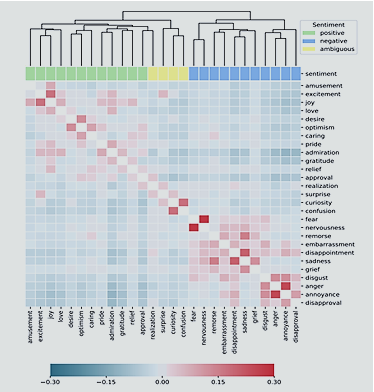
\includegraphics[width=0.55\textwidth]{figures/image16}
  \caption{Correlation and Hierarchical clustering of emotions and their rating \cite{ref77}}
  \label{fig:ch3_f2}
\end{figure}

\section{Results and Discussion}
For evaluating emotion prediction models, the metrics are Precision, Recall, and F1 Score. Although the GoEmotions dataset labeled Reddit comments with 27 emotions, we considered only 12 emotions that are strongly identified.

\subsubsection*{Performance Analysis}
We compare the final results of BERT, Plain PRADO, and FL-PRADO, implemented using the environment discussed in Section 3.3. As per the setup mentioned in Section 3.3, the federated configuration of FL-PRADO includes 120 clients. The GoEmotions dataset is divided into 43,410 training examples and 5,427 test examples over 28 emotions. The BERT and PRADO models are using the dataset as per the train and test split mentioned here. On the other hand, this dataset is divided across 120 clients with approximately 360-365 examples each (seeded permutation, persisted) for FL-PRADO. Precision and Recall were chosen, along with F1 score, due to the nature of emotion recognition being a multi-class classification problem, where a class imbalance can be misleading. These are complementary indicators of how well the model is able to correctly recognize emotions, capture the true emotion instances, and to balance both. For the GoEmotions-based FL-PRADO experiment, Macro-F1 can be especially valuable because it gives each emotion class equal importance, including less frequent emotions.

\subsection{Precision Comparison}
Precision of a model is stated as the proportion of its positive predictions that turn out to be true.

\begin{equation}
  \text{Precision} = \frac{TP}{TP + FP}
  \label{eq:ch3_precision}
\end{equation}

\noindent Where $TP$ is the number of true positives and $FP$ is the number of false positives.

Recall measures the proportion of correct positive predictions out of all actual positives in the data.

\begin{equation}
  \text{Recall} = \frac{TP}{TP + FN}
  \label{eq:ch3_recall}
\end{equation}

\noindent Where $FN$ is the number of false negatives.

The F1-score provides a balanced assessment, considering both Precision and Recall.

\begin{equation}
  \text{F1 Score} = \frac{2 \times \text{Precision} \times \text{Recall}}{\text{Precision} + \text{Recall}}
  \label{eq:ch3_f1}
\end{equation}

\begin{table}[htbp]
  \centering
  \caption{Precision scores for the prediction of emotions}
  \label{tab:ch3_t1}
  \begin{tabular}{|c|c|c|c|}
    \hline
    Emotion & Precision (Small BERT) & Precision PRADO & Precision  FL-PRADO \\
    \hline
    Desire & 0.600 & 0.553 & 0.529 \\
    \hline
    Excitement & 0.667 & 0.710 & 0.278 \\
    \hline
    Amusement & 0.724 & 0.725 & 0.724 \\
    \hline
    Anger & 0.561 & 0.602 & 0.522 \\
    \hline
    Admiration & 0.702 & 0.602 & 0.431 \\
    \hline
    Gratitude & 0.932 & 0.950 & 0.966 \\
    \hline
    Remorse & 0.545 & 0.527 & 0.500 \\
    \hline
    Joy & 0.482 & 0.551 & 0.536 \\
    \hline
    Sadness & 0.562 & 0.594 & 0.461 \\
    \hline
    Love & 0.767 & 0.782 & 0.536 \\
    \hline
    Optimism & 0.713 & 0.713 & 0.680 \\
    \hline
    Neutral & 0.645 & 0.612 & 0.467 \\
    \hline
  \end{tabular}
\end{table}

Table 3.1 displays the precision scores for predicting emotions using three different model setups: Baseline 1 (BERT), Baseline 2 (the original PRADO model); and the PRADO model used in an FL context(FL-PRADO .

\begin{figure}[htbp]
  \centering
  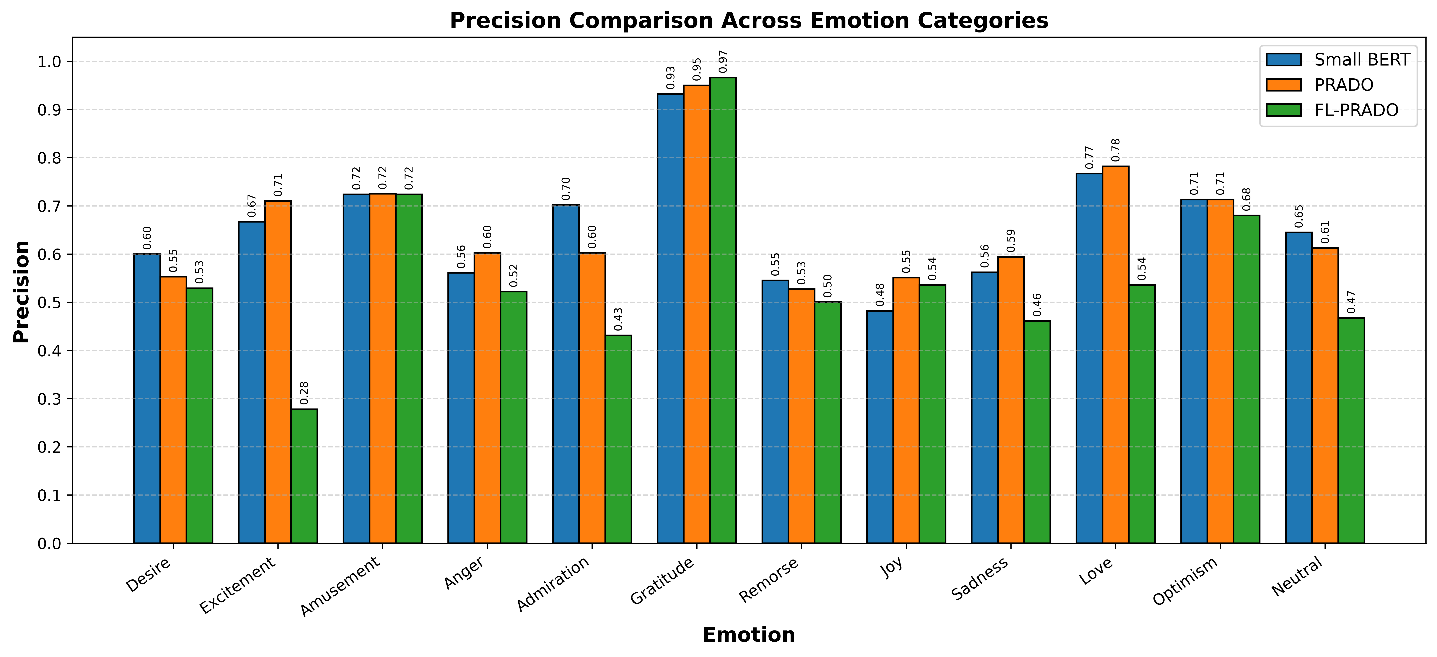
\includegraphics[width=0.8\textwidth]{figures/image17}
  \caption{Precision comparison with base models}
  \label{fig:ch3_f3}
\end{figure}

The bar chart compares the precision scores for predicting emotions using three different model setups: Baseline 1 (BERT), Baseline 2 (with PRADO only), and PRADO used in a Federated Learning (FL) environment. It examines twelve emotions, from admiration to sadness, to assess how well the models can predict whether someone is feeling good. The green bars representing FL-PRADO maintain competitive precision across several emotions while preserving privacy in an FL environment, consistently achieving better precision scores for most emotions. However, the macro-average precision for 27 emotions is lower than that of baseline models.

\subsection{Recall Comparison}
Recall measures the proportion of correct positive predictions out of all actual positives in the data.

As discussed in the dataset limitations, certain emotions have fewer examples than others. Training and Evaluation of the models are affected by this.

Table 3.3 and the bar chart in Figure 3.4 compare recall values for three model configurations across twelve emotional categories. This comparison differs from the earlier precision-focused figure. It shows that FL-PRADO consistently has the highest recall for most emotions.

\begin{table}[htbp]
  \centering
  \caption{Recall@5 score evaluation for emotion prediction}
  \label{tab:ch3_t2}
  \begin{tabular}{|c|c|c|c|}
    \hline
    Emotion & Recall (BERT)- & Recall (PRADO) & Recall (FL-PRADO) \\
    \hline
    Admiration & 0.444 & 0.489 & 0.574 \\
    \hline
    Joy & 0.168 & 0.503 & 0.566 \\
    \hline
    Anger & 0.162 & 0.288 & 0.292 \\
    \hline
    Desire & 0.145 & 0.313 & 0.317 \\
    \hline
    Excitement & 0.117 & 0.214 & 0.149 \\
    \hline
    Gratitude & 0.821 & 0.858 & 0.898 \\
    \hline
    Optimism & 0.306 & 0.468 & 0.476 \\
    \hline
    Love & 0.622 & 0.786 & 0.788 \\
    \hline
    Neutral & 0.558 & 0517 & 0.618 \\
    \hline
    Remorse & 0.321 & 0.696 & 0.589 \\
    \hline
    Sadness & 0.231 & 0.263 & 0.263 \\
    \hline
    Amusement & 0.526 & 0.658 & 0.665 \\
    \hline
  \end{tabular}
\end{table}

Figure 3.4 shows a comparison of Recall for all 3 models mentioned across twelve emotions.  FL PRADO has much better recall values. For example, the recall for admiration (0.574), gratitude (0.898), and joy (566) indicates stricter classification boundaries.

\begin{figure}[htbp]
  \centering
  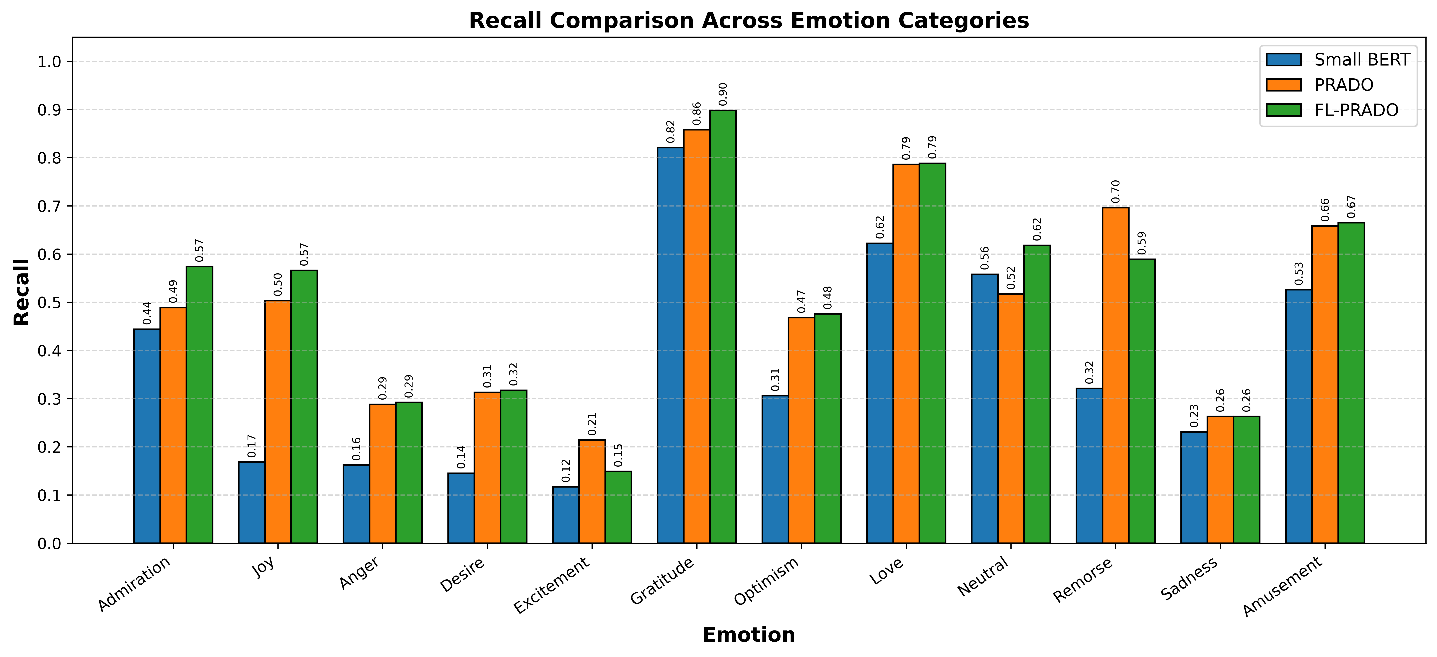
\includegraphics[width=0.8\textwidth]{figures/image18}
  \caption{Recall comparison with base models}
  \label{fig:ch3_f4}
\end{figure}

This higher recall can be beneficial in personalized emotion-based recommendation systems, where offering unrelated emotional content may harm user experience more than omitting a few items. In federated settings, stronger local model behavior also helps protect privacy and reduces noise during aggregation, leading to more accurate and personalized results. Therefore, FL PRADO produces highly reliable predictions, which is crucial for emotion models used in privacy-sensitive applications.

\subsection{F1 Score Comparison}
The F1-score provides a balanced assessment. It considers both Precision and Recall. It is formulated as shown.

The F1 score comparison graph in Figure 3.5 and Table 3.4 shows how well emotion prediction models perform across three different settings: Baseline 1 (BERT), Baseline 2 (PRADO), and FL-PRADO. Baseline 1 has a better F1 score for some emotions. Baseline 2 shows that PRADO has a positive effect on prediction quality in a federation-free system. The PRADO-FL system remains competitive across key emotions such as gratitude, love, and neutrality, demonstrating PRADO's flexibility amid federation constraints. An emotion such as excitement would probably not work, as the data is limited and different for local FL training.

\begin{table}[htbp]
  \centering
  \caption{F1-Score Comparison with Base Models}
  \label{tab:ch3_t3}
  \begin{tabular}{|c|c|c|c|}
    \hline
    Emotion & F1 Score (BERT) & F1 Score (PRADO) & F1 Score (FL-PRADO) \\
    \hline
    Admiration & 0.544 & 0.596 & 0.452 \\
    \hline
    Gratitude & 0.873 & 0.901 & 0.886 \\
    \hline
    Anger & 0.251 & 0.369 & 0.351 \\
    \hline
    Desire & 0.233 & 0.4 & 0.308 \\
    \hline
    Excitement & 0.198 & 0.328 & 0.083 \\
    \hline
    Amusement & 0.610 & 0.596 & 0.452 \\
    \hline
    Joy & 0.249 & 0.523 & 0.435 \\
    \hline
    Love & 0.687 & 0.784 & 0.784 \\
    \hline
    Neutral & 0.598 & 0.561 & 0.588 \\
    \hline
    Optimism & 0.429 & 0.565 & 0.484 \\
    \hline
    Remorse & 0.404 & 0.6 & 0.569 \\
    \hline
    Sadness & 0.327 & 0.364 & 0.355 \\
    \hline
  \end{tabular}
\end{table}

\begin{figure}[htbp]
  \centering
  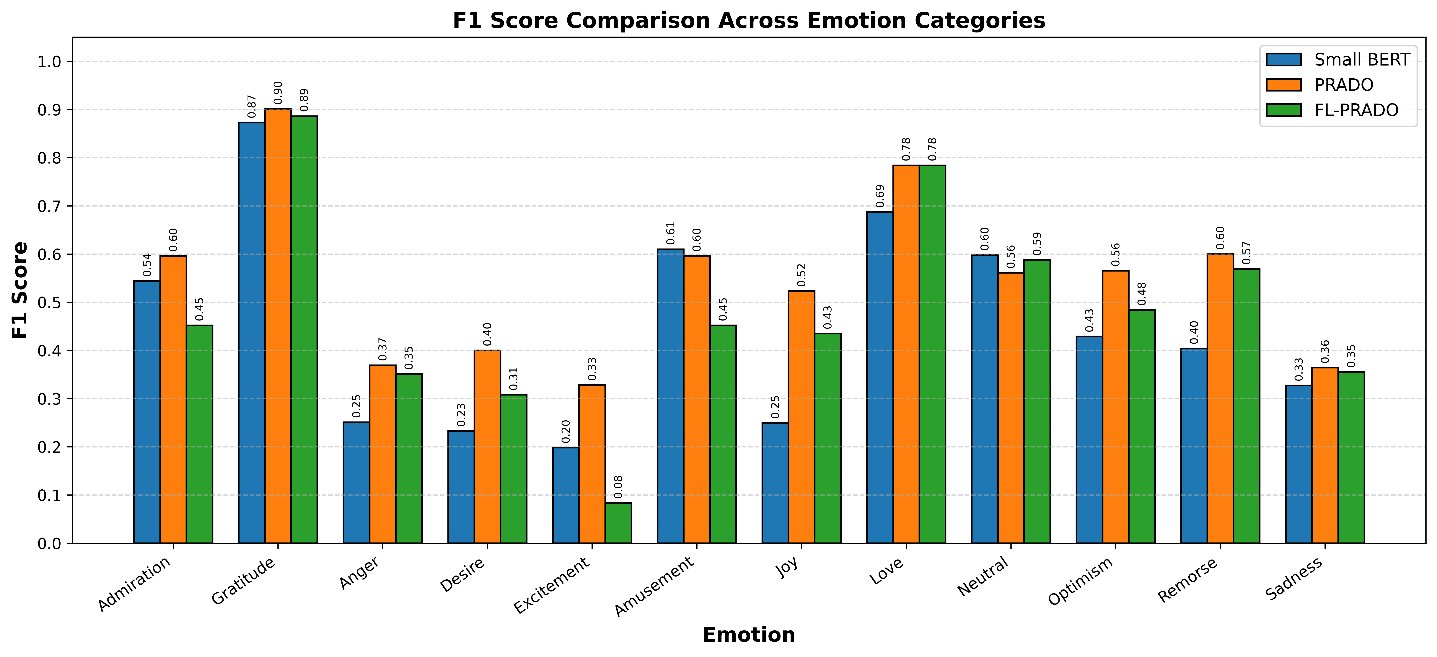
\includegraphics[width=0.8\textwidth]{figures/image19}
  \caption{F1 Score Comparison with Base Models}
  \label{fig:ch3_f5}
\end{figure}

\subsection{Evaluation of Emotion Prediction}
We first run the baseline models---LSTM \cite{ref84}, Bi-LSTM \cite{ref85} , BERT\cite{ref67} , and PRADO---in a non-federated learning (FL) setting. For on-device applications, PRADO's strength is its ability to function well with low memory and processing power. The estimated precision, recall, and F1-score values for various language models are displayed in Table 5.1.

\begin{table}[htbp]
  \centering
  \caption{Emotion prediction analysis using the GoEmotions dataset}
  \label{tab:ch3_t4}
  \begin{tabular}{|c|c|c|c|c|c|}
    \hline
    Model & Setting & Test loss (BCE) & Precision@0.5 & Recall@0.5 & F1-score \\
    \hline
    BERT & centralized & --- & 0.679 & 0.351 & 0.463 \\
    \hline
    PRADO & (on device) & 0.327 & 0.630 & 0.392 & 0.483 \\
    \hline
    LSTM & centralized & --- & 0.642 & 0.351 & 0.453 \\
    \hline
    Bi-LSTM & centralized & --- & 0.673 & 0.292 & 0.407 \\
    \hline
    BERT FL & federated & 0.138 & 0.596 & 0.256 & 0.358 \\
    \hline
    PRADO FL & federated & 0.174 & 0.467 & 0.476 & 0.472 \\
    \hline
  \end{tabular}
\end{table}

Every baseline model---LSTM, Bi-LSTM, BERT, and PRADO---is executed in a typical, non-FL setting. Compared to other models, FL-PRADO exhibits notable advancements in Recall and F1 score. We computed the 95\% confidence intervals (CI) for accuracy, recall, and F1-score to give a statistical measure of their dependability and variability. The models were re-evaluated on random subsets of the test set at ten sizes (10\%, 20\%, $\ldots$ 100\%), and their 95\% confidence intervals were obtained by bootstrapping $B = 1{,}000$ resamples within that subset.  Various clients and training cycles are represented by weighted-average scores of various variables in Tables 3.5(a)--3.5(c) and Figures 3.6(a)--3.6(c).

\setlength{\tabcolsep}{4pt}
\begin{longtable}{|p{1.9cm}|p{1.9cm}|p{1.9cm}|p{1.9cm}|p{1.9cm}|p{1.9cm}|p{1.9cm}|}
\caption{Weighted-averaged Precision: realized value on each evaluation subset}
\label{tab:ch3_t5} \\
\hline
Eval. size & BERT & PRADO & LSTM & Bi-LSTM & BERT FL & PRADO FL \\
\hline
\endfirsthead
\hline
Eval. size & BERT & PRADO & LSTM & Bi-LSTM & BERT FL & PRADO FL \\
\hline
\endhead
\hline
\endfoot
10\% / (n=543) & 0.645 / {[0.568, 0.706]} & 0.562 / {[0.479, 0.613]} & 0.527 / {[0.450, 0.589]} & 0.284 / {[0.244, 0.329]} & 0.324 / {[0.247, 0.373]} & 0.394 / {[0.356, 0.447]} \\
\hline
20\% / (n=1,085) & 0.621 / {[0.559, 0.661]} & 0.537 / {[0.482, 0.587]} & 0.573 / {[0.522, 0.620]} & 0.385 / {[0.332, 0.419]} & 0.355 / {[0.320, 0.391]} & 0.438 / {[0.407, 0.474]} \\
\hline
30\% / (n=1,628) & 0.669 / {[0.631, 0.707]} & 0.549 / {[0.514, 0.596]} & 0.583 / {[0.527, 0.631]} & 0.357 / {[0.310, 0.382]} & 0.379 / {[0.320, 0.407]} & 0.437 / {[0.410, 0.462]} \\
\hline
40\% / (n=2,171) & 0.676 / {[0.619, 0.709]} & 0.522 / {[0.499, 0.551]} & 0.596 / {[0.536, 0.621]} & 0.332 / {[0.310, 0.356]} & 0.377 / {[0.324, 0.399]} & 0.456 / {[0.422, 0.482]} \\
\hline
50\% / (n=2,714) & 0.615 / {[0.579, 0.654]} & 0.552 / {[0.518, 0.595]} & 0.598 / {[0.549, 0.625]} & 0.359 / {[0.313, 0.378]} & 0.379 / {[0.331, 0.400]} & 0.434 / {[0.410, 0.452]} \\
\hline
60\% / (n=3,256) & 0.667 / {[0.618, 0.695]} & 0.534 / {[0.515, 0.557]} & 0.591 / {[0.539, 0.614]} & 0.365 / {[0.323, 0.383]} & 0.382 / {[0.333, 0.402]} & 0.463 / {[0.425, 0.482]} \\
\hline
70\% / (n=3,799) & 0.657 / {[0.630, 0.687]} & 0.553 / {[0.521, 0.589]} & 0.590 / {[0.547, 0.612]} & 0.364 / {[0.323, 0.380]} & 0.379 / {[0.334, 0.397]} & 0.452 / {[0.424, 0.474]} \\
\hline
80\% / (n=4,342) & 0.656 / {[0.622, 0.687]} & 0.540 / {[0.515, 0.574]} & 0.582 / {[0.546, 0.607]} & 0.367 / {[0.330, 0.384]} & 0.389 / {[0.344, 0.406]} & 0.446 / {[0.425, 0.469]} \\
\hline
90\% / (n=4,884) & 0.657 / {[0.625, 0.687]} & 0.558 / {[0.528, 0.592]} & 0.596 / {[0.558, 0.618]} & 0.372 / {[0.330, 0.387]} & 0.385 / {[0.341, 0.400]} & 0.446 / {[0.425, 0.468]} \\
\hline
100\% / (n=5,427) & 0.656 / {[0.627, 0.684]} & 0.549 / {[0.520, 0.582]} & 0.592 / {[0.555, 0.614]} & 0.365 / {[0.328, 0.378]} & 0.380 / {[0.336, 0.396]} & 0.457 / {[0.430, 0.475]} \\
\hline
\end{longtable}

The weighted-averaged precision with 95\% confidence intervals (CI) for BERT, LSTM, Bi-LSTM, PRADO, and FL-PRADO across different dataset sizes is shown in Fig.  3.2(a). Compared to FL models, BERT, PRADO, and Bi-LSTM demonstrate higher precision. As the evaluation set size increases, the confidence intervals narrow. FL-PRADO achieves the best recall results for all evaluation-set sizes. The model's high recall across all iterations indicates greater sensitivity to the positive emotion classes in the federated learning framework, which helps maintain predictive capacity while minimizing missed detections. The 95\% half-width of the weighted F1 is reduced from around $\pm 0.035$--$0.041$ at 10\% of the test set to $\pm 0.012$--$0.013$ at the full test set. The interval width doesn't shrink monotonically over all models, due to the different random subset of evaluations used by each evaluation size.

\begin{figure}[htbp]
  \centering
  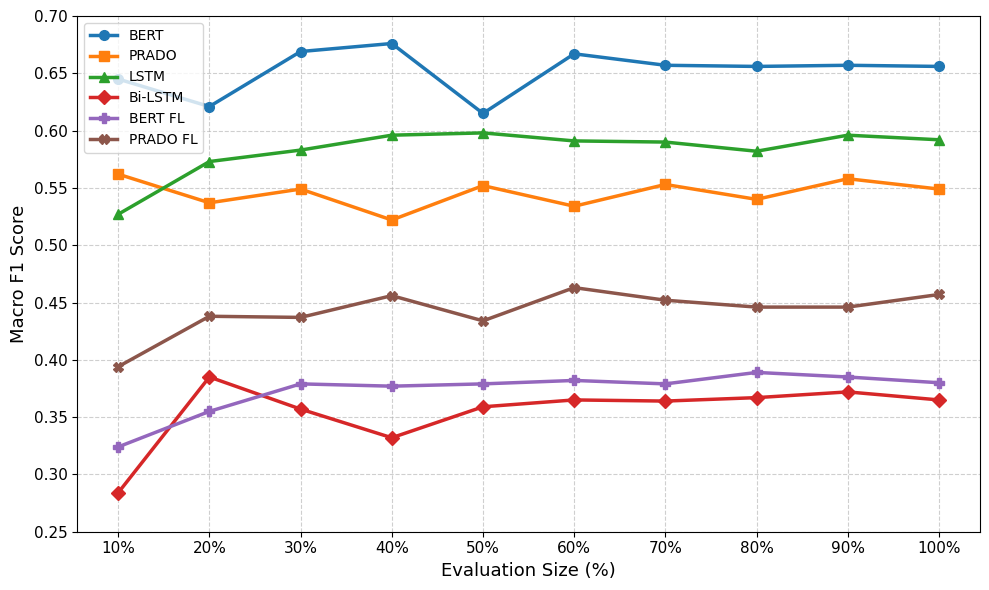
\includegraphics[width=\textwidth]{figures/image20}
  \caption{Weighted-averaged precision with 95\% CI for different models}
  \label{fig:ch3_f6}
\end{figure}

\begin{longtable}{|p{1.9cm}|p{1.9cm}|p{1.9cm}|p{1.9cm}|p{1.9cm}|p{1.9cm}|p{1.9cm}|}
\caption{Weighted-averaged Recall: realized value on each evaluation subset}
\label{tab:ch3_t6} \\
\hline
Eval. Size & BERT & PRADO & LSTM & Bi-LSTM & BERT FL & PRADO FL \\
\hline
\endfirsthead
\hline
Eval. Size & BERT & PRADO & LSTM & Bi-LSTM & BERT FL & PRADO FL \\
\hline
\endhead
\hline
\endfoot
10\% / (n=543) & 0.350 / {[0.313, 0.385]} & 0.387 / {[0.348, 0.428]} & 0.352 / {[0.318, 0.388]} & 0.269 / {[0.236, 0.302]} & 0.234 / {[0.200, 0.268]} & 0.460 / {[0.422, 0.500]} \\
\hline
20\% / (n=1,085) & 0.341 / {[0.317, 0.369]} & 0.398 / {[0.372, 0.425]} & 0.380 / {[0.353, 0.407]} & 0.311 / {[0.286, 0.337]} & 0.262 / {[0.238, 0.288]} & 0.498 / {[0.468, 0.526]} \\
\hline
30\% / (n=1,628) & 0.349 / {[0.329, 0.370]} & 0.395 / {[0.375, 0.420]} & 0.346 / {[0.324, 0.370]} & 0.280 / {[0.261, 0.301]} & 0.246 / {[0.228, 0.269]} & 0.471 / {[0.449, 0.494]} \\
\hline
40\% / (n=2,171) & 0.349 / {[0.331, 0.369]} & 0.392 / {[0.371, 0.409]} & 0.346 / {[0.326, 0.363]} & 0.283 / {[0.264, 0.301]} & 0.254 / {[0.237, 0.273]} & 0.473 / {[0.454, 0.493]} \\
\hline
50\% / (n=2,714) & 0.349 / {[0.333, 0.367]} & 0.390 / {[0.374, 0.408]} & 0.349 / {[0.332, 0.365]} & 0.290 / {[0.274, 0.306]} & 0.250 / {[0.234, 0.265]} & 0.466 / {[0.448, 0.483]} \\
\hline
60\% / (n=3,256) & 0.361 / {[0.345, 0.376]} & 0.401 / {[0.387, 0.417]} & 0.352 / {[0.338, 0.367]} & 0.293 / {[0.279, 0.308]} & 0.259 / {[0.246, 0.274]} & 0.481 / {[0.464, 0.497]} \\
\hline
70\% / (n=3,799) & 0.354 / {[0.340, 0.370]} & 0.390 / {[0.376, 0.404]} & 0.353 / {[0.339, 0.368]} & 0.294 / {[0.281, 0.308]} & 0.259 / {[0.245, 0.273]} & 0.474 / {[0.459, 0.489]} \\
\hline
80\% / (n=4,342) & 0.353 / {[0.337, 0.366]} & 0.392 / {[0.378, 0.405]} & 0.353 / {[0.340, 0.365]} & 0.292 / {[0.280, 0.305]} & 0.260 / {[0.247, 0.271]} & 0.480 / {[0.467, 0.494]} \\
\hline
90\% / (n=4,884) & 0.354 / {[0.341, 0.367]} & 0.396 / {[0.384, 0.410]} & 0.353 / {[0.341, 0.365]} & 0.296 / {[0.284, 0.308]} & 0.257 / {[0.245, 0.269]} & 0.480 / {[0.468, 0.494]} \\
\hline
100\% / (n=5,427) & 0.351 / {[0.340, 0.364]} & 0.392 / {[0.381, 0.404]} & 0.351 / {[0.339, 0.362]} & 0.292 / {[0.280, 0.304]} & 0.256 / {[0.245, 0.266]} & 0.476 / {[0.464, 0.489]} \\
\hline
\end{longtable}

\begin{figure}[htbp]
  \centering
  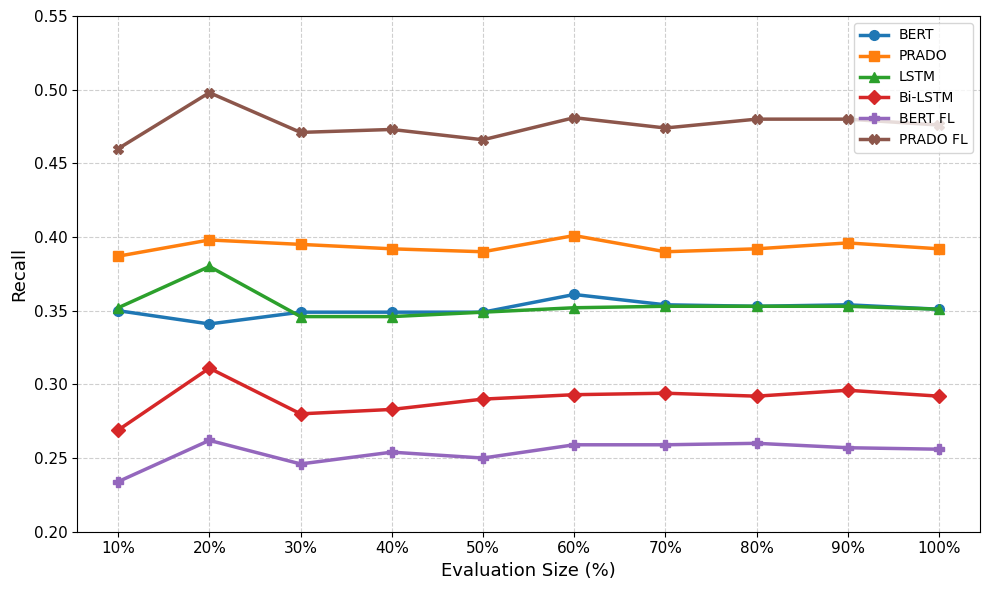
\includegraphics[width=\textwidth]{figures/image21}
  \caption{Weighted-averaged Recall with 95\% confidence intervals}
  \label{fig:ch3_f7}
\end{figure}

\begin{longtable}{|p{1.9cm}|p{1.9cm}|p{1.9cm}|p{1.9cm}|p{1.9cm}|p{1.9cm}|p{1.9cm}|}
\caption{Weighted-averaged F1: realized value on each evaluation subset}
\label{tab:ch3_t7} \\
\hline
Eval. size & BERT & PRADO & LSTM & Bi-LSTM & BERT FL & PRADO FL \\
\hline
\endfirsthead
\hline
Eval. size & BERT & PRADO & LSTM & Bi-LSTM & BERT FL & PRADO FL \\
\hline
\endhead
\hline
\endfoot
10\% / (n=543) & 0.408 / {[0.365, 0.443]} & 0.420 / {[0.379, 0.462]} & 0.385 / {[0.344, 0.424]} & 0.275 / {[0.240, 0.311]} & 0.237 / {[0.203, 0.272]} & 0.387 / {[0.348, 0.427]} \\
\hline
20\% / (n=1,085) & 0.400 / {[0.371, 0.430]} & 0.433 / {[0.404, 0.460]} & 0.423 / {[0.392, 0.451]} & 0.331 / {[0.304, 0.359]} & 0.265 / {[0.237, 0.293]} & 0.426 / {[0.397, 0.454]} \\
\hline
30\% / (n=1,628) & 0.418 / {[0.394, 0.441]} & 0.434 / {[0.413, 0.458]} & 0.393 / {[0.367, 0.416]} & 0.301 / {[0.279, 0.323]} & 0.260 / {[0.239, 0.284]} & 0.407 / {[0.385, 0.430]} \\
\hline
40\% / (n=2,171) & 0.406 / {[0.385, 0.426]} & 0.427 / {[0.407, 0.446]} & 0.392 / {[0.369, 0.411]} & 0.303 / {[0.284, 0.322]} & 0.260 / {[0.242, 0.280]} & 0.410 / {[0.390, 0.431]} \\
\hline
50\% / (n=2,714) & 0.407 / {[0.388, 0.427]} & 0.430 / {[0.413, 0.448]} & 0.392 / {[0.374, 0.409]} & 0.306 / {[0.289, 0.323]} & 0.261 / {[0.244, 0.277]} & 0.402 / {[0.385, 0.419]} \\
\hline
60\% / (n=3,256) & 0.423 / {[0.405, 0.439]} & 0.439 / {[0.423, 0.455]} & 0.398 / {[0.380, 0.414]} & 0.312 / {[0.296, 0.328]} & 0.269 / {[0.255, 0.285]} & 0.417 / {[0.400, 0.433]} \\
\hline
70\% / (n=3,799) & 0.417 / {[0.401, 0.433]} & 0.430 / {[0.414, 0.446]} & 0.397 / {[0.382, 0.413]} & 0.312 / {[0.297, 0.327]} & 0.268 / {[0.254, 0.283]} & 0.409 / {[0.394, 0.423]} \\
\hline
80\% / (n=4,342) & 0.414 / {[0.399, 0.429]} & 0.433 / {[0.418, 0.446]} & 0.399 / {[0.384, 0.413]} & 0.312 / {[0.298, 0.326]} & 0.271 / {[0.258, 0.284]} & 0.415 / {[0.401, 0.429]} \\
\hline
90\% / (n=4,884) & 0.417 / {[0.404, 0.431]} & 0.437 / {[0.423, 0.451]} & 0.400 / {[0.385, 0.412]} & 0.316 / {[0.303, 0.329]} & 0.270 / {[0.258, 0.283]} & 0.415 / {[0.402, 0.429]} \\
\hline
100\% / (n=5,427) & 0.413 / {[0.400, 0.426]} & 0.433 / {[0.419, 0.444]} & 0.396 / {[0.383, 0.408]} & 0.311 / {[0.298, 0.323]} & 0.267 / {[0.255, 0.279]} & 0.411 / {[0.398, 0.423]} \\
\hline
\end{longtable}
\setlength{\tabcolsep}{6pt}

\begin{figure}[htbp]
  \centering
  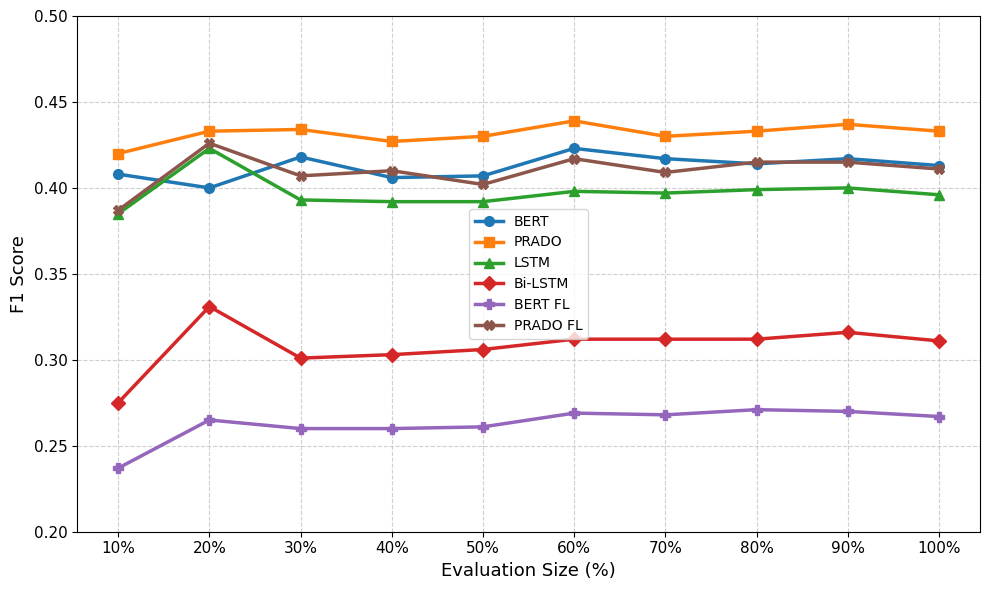
\includegraphics[width=\textwidth]{figures/image22}
  \caption{Weighted-averaged F1 score with 95\% confidence intervals}
  \label{fig:ch3_f8}
\end{figure}

\section{Detailed Analysis of Work}
This section provides details regarding the selection of models for comparison and the performance of the proposed model for research. The purpose of this experimentation is to check the suitability of PRADO in the FL framework.

\subsection{Model Selection for 12 strongly identified emotions Comparison}
The proposed work compares FL-PRADO, BERT, and PRADO. All three models are trained on the GoEmotions dataset using the setup given in Section 3.3. The BERT model is a representative pre-trained transformer model and is also used by the authors of PRADO for comparison. Considering the challenges of FL environment, \cite{ref28} and the lightweight projection-based architecture of PRADO, we integrated it into the FL framework. To assess the performance of the proposed model only for emotion prediction, the models required should be common in the dataset used for training. Hence, BERT is selected as a representative transformer model, and PRADO is selected as it is ideal for its lightweight framework. The proposed model can be compared with other SOTA models for emotion prediction, but these models are either using centralized machine learning without considering user privacy or FL models that use different datasets and provide no publicly available implementation details to reproduce them. To create a common platform for further research work, these three models were implemented and assessed across Precision, Recall, and F1.

\subsection{Performance discussion of proposed model}
The objective of FL-PRADO is not only to enhance evaluation metrics, but also to address three practical requirements: First, privacy preservation by ensuring that the user’s original data never leaves the local device. Second, lightweight deployment using PRADO is most suitable for edge devices participating in federated learning. Third, the work carried out in this chapter demonstrated scalable collaborative learning across 120 distributed clients.

Considering these requirements, the performance of FL-PRADO is justifiable. The precision analysis over several emotions produces competitive performance (desire, amusement, anger, gratitude, etc.), though the macro average is poor. FL-PRADO achieves the highest recall for most emotions, and the performance of FL-PRADO is very close to the performance of PRADO for F1-Score.

\section{Summary}
In this chapter, we proposed a framework for privacy-preserving emotion recognition, called FL-PRADO. It included a detailed description of the PRADO architecture, the federation aggregation process, the experimental setup, dataset partitioning, and the GoEmotions dataset. The effectiveness of the proposed model was tested in terms of Precision, recall, and F1 score. The results were compared with baseline models. The results show that FL-PRADO can make competitive emotion prediction without compromising user privacy and enables efficient deployment on edge devices. These emotion predictions are used in the following chapter to create the proposed cross-domain recommendation framework. The work described in this chapter demonstrates the accomplishment of the first and second objectives. According to a research survey, no federated learning framework has been implemented using PRADO for emotion prediction.


\chapter{Multi-Objective and Modular Federated Cross-Domain Recommendation}
The proposed research work presents an emotion-aware cross-domain recommendation system that utilizes the GoEmotions dataset and curated datasets across different domains such as movies, music, games, and books, and produces personalized recommendations using emotional information derived from user-generated reviews and textual content. A detailed case study across these four domains is used to test the framework and show how it can capture user emotional preferences. Traditional recommendation systems are mainly based on user behavior (ratings, browsing history, user interactions) and item attributes (genre, author, artist, developer, etc.). But feelings are intrinsically linked to user preferences and consumption decisions. The proposed framework leverages emotion analysis to provide more personalized and contextually relevant recommendations for books, movies, music, and games, ultimately improving user satisfaction and recommendation relevance.

In the previous chapter, the focus was on user emotion recognition, which is used to develop the proposed model. The proposed multi-objective Federated cross-domain recommendation system extracts user emotions from their reviews. The emotions from user reviews are transformed for the recommendation model.

\section{Federated Cross-Domain Recommendation}
Providing effective service or product recommendations requires a lot of user data. This data should comprise contextual and behavioral data. A user's interests can span various areas, particularly when a user communicates with a wide range of platforms. The preferences in different domains must be elicited by a CDR system, which is essential in the recommendations of appropriate products. The richness of information sources will allow CDR systems to propose products in cases where there is a lack of domain-specific data or none at all. Onboarding a new user or cold starting is a problem that CDR systems have managed effectively. However, there is a risk of privacy leakage because the process involves exchanging data between domains, particularly between source and target sites. Many consumers may choose not to share their information due to the rising enforcement of privacy laws such as GDPR, CCPA, and others. FL complies with these legal requirements by minimizing disclosures of data, and giving users increased control over their data. The study suggests the real-time use of a Federated Learning model that effectively controls the transmission of client data to the server. Implementing the Projected Attention Network (PRADO) in the FL environment successfully overcomes resource constraints on edge devices during model training. The strategy can address resource limitations, including computing power, memory, and battery life, on edge devices. FL transfer learning is also applied to provide cross-domain recommendations through an enhanced recommender. Cosine similarity is used in the recommender system to find items with emotional representations similar to the user's inferred emotional profile. Unlike conventional recommendation methods like collaborative filtering or matrix factorization, cosine similarity works directly on learned emotional embeddings, allowing it to perform well even if there is not much explicit data regarding user--item interactions. It overcomes cold-start and data-sparsity challenges with a different approach: it compares semantic similarity in the embedding space instead of past interactions. Embedding PRADO at the local layer and using an enhanced recommender in the FL environment make the system modular, scalable, and cost-effective. This approach improves recommendation performance in the FL environment and surpasses baseline models. The proposed system provides the benefits listed below over prior approaches.

The PRADO model was trained using the Go emotions dataset, and the attention distribution was computed for samples from the test set. The words with the closest attention are extracted and categorized. In this case, the vocabulary is not manually selected for the data; instead, the model automatically learns to categorize words by emotion using trained projections.

This approach results in a compact neural network with less memory, which is further optimized, helping to speed up on-device training at runtime.

The pre-trained PRADO model is used for transfer learning in a federated learning environment. The projection embeddings trained for emotions using the Go Emotion dataset from different clients in FL are sent to the server for buffered/weighted federated averaging. The updated parameters are successfully applied to the target domain for recommendation with limited training data. Integrating enhanced recommenders speeds up model training and handles noisy data effectively.

The chapter's contributions are described below:

\begin{enumerate}
    \item The proposed system combines the Projected Attention Network (PRADO) with an FL framework to predict emotions as the source domain.
    \item The research implements a novel Fed CDR architecture that combines Federated transfer learning with an enhanced recommender. The hybrid approach uses transfer learning to provide rich contextual understanding with limited resources across domains, improving the model's performance.
    \item The empirical evaluation demonstrates that the multi-objective and modular Federated Cross-Domain Recommendation System (MFCDR) outperforms the baseline and SOTA models.
\end{enumerate}

\section{Problem Statement}
Consider a scenario where a centralized server and $M$ local clients are involved in the training process. The clients signify individual users, denoted by the set $U = \{u_1, u_2, \ldots, u_m\}$. For each user $u_i$, an emotion embedding vector $e \in \mathbb{R}^{d}$ is extracted from their reviews, forming the set of user emotions $E = \{e_1, e_2, \ldots, e_m\}$. Let $T = \{t_1, t_2, \ldots, t_n\}$ be the set of target domains, and let $V = \{v_1, v_2, \ldots, v_n\}$ denote the corresponding set of review texts associated with each item. The primary goal is to predict the appropriate emotion vector $e_i$ for each user and recommend the most relevant target item $t_j \in T$ whose reviews semantically match the user's emotional profile.

\section{Proposed method for Multi-Objective, Modular FedCDR using PRADO}
The proposed method involves Projected Attention Network (PRADO), which is outlined in Chapter 3. PRADO combines trainable projection layers, attention processes, and convolutional processes to enable the model to efficiently extract semantic and contextual information from the input data. The biggest strength of PRADO is its ability to process and categorize long text sequences with high precision and effectiveness. The architecture is particularly applicable in environments where user reviews are lengthy or complex emotional expressions are to be documented. With PRADO's powerful long-text processing capabilities, the proposed system greatly improves the performance and accuracy of the emotion-based recommendation task and makes the proposed suggestions to the user more accurate and context-sensitive \cite{ref37}. Figure 4.1 represents an architecture of the proposed model. It consists of the following modules:

\begin{itemize}
    \item Emotion Prediction module at the Local Layer
    \item Buffered/Weighted FedAvg Aggregator
    \item Recommendation Module
\end{itemize}

\subsection{Emotion Prediction module at the Local Layer}
This layer facilitates training local models, with each user acting as a distinct client. Due to the resource constraints common in edge devices in federated learning (FL) environments, the PRADO is used to overcome these limitations \cite{ref75}.

In traditional NLP pipelines, each word is usually represented by a one-hot encoded vector and the vector length equals the size of the vocabulary (|V|). The vector has one element corresponding to the target word, set to 1, while other elements are 0. These vectors become sparse and cannot capture relationships among words. Hence, they are transformed into dense word embeddings. The word embedding matrix W and the embedding of the ith word is represented as

where is the one-hot encoded vector and is the resulting dense word embedding. This approach needs considerable memory resources for storing large embedding matrices, which makes it impractical for resource-limited devices involved in FL. PRADO addresses this challenge by replacing the standard embedding layer with a projection-based approach (discussed at length in Chapter 3), significantly reducing memory usage while preserving model performance.

\subsection{Buffered/Weighted FedAvg Aggregator}
In Federated Learning, every client maintains its own local dataset and uses the Projected Attention Network (PRADO) to train a local model. The locally trained models from each participating client are then combined to update the global Model ''W''. Various communication protocols have been proposed for model aggregation, including synchronous, semi-synchronous \cite{ref79}, and asynchronous methods \cite{ref80} . These methods, however, frequently don't work well in heterogeneous settings. For example, in synchronous protocols, faster clients may have to wait for slower ones, thereby inefficiently using computational resources. Conversely, asynchronous methods allow clients to update independently, which improves resource utilization, but they significantly increase network communication overhead  \cite{ref44}.

\begin{figure}[htbp]
  \centering
  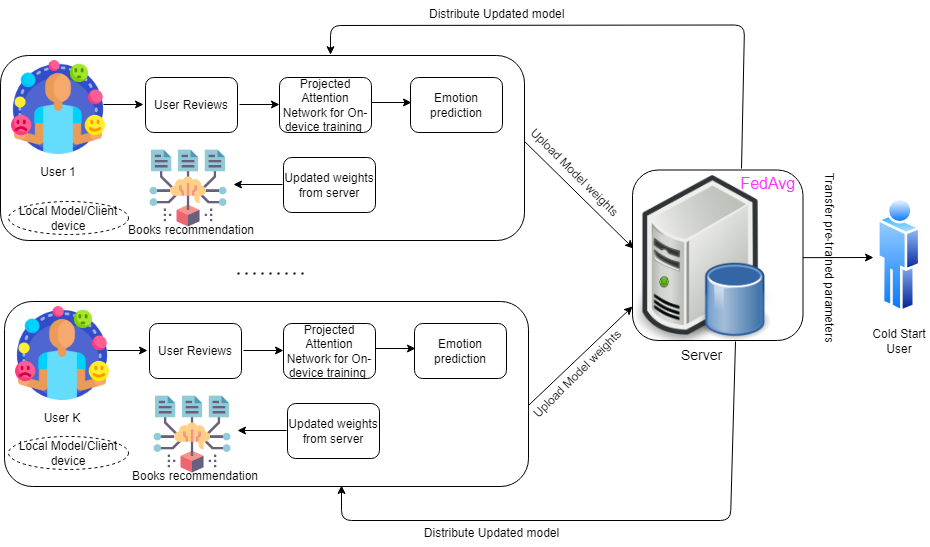
\includegraphics[width=0.8\textwidth]{figures/image23}
  \caption{Architecture of a Modular Federated Cross-Domain Recommendation System based on PRADO}
  \label{fig:ch4_f1}
\end{figure}

To tackle these limitations, a hybrid strategy, Buffered FedAvg, is used for global model training \cite{ref80} . In this approach, the server does not immediately combine the model after receiving each client's update. Instead, it temporarily saves the updates in a buffer. Only when the buffer reaches a predetermined threshold, M, does aggregation take place. That is, the server updates the model only after receiving M client updates, as shown in the following equation.

\begin{equation}
  w_{\text{server}}^{t+1}(\text{aggr}_{p}) = \frac{1}{M} \sum_{i \in B_{t}} w_{i}^{t}, \quad |B_{t}| \geq M
  \label{eq:ch4_4_1}
\end{equation}

$\mathbf{w}_{\text{global}}^{t+1}$ --- Aggregated global model parameters at round $t+1$.

$\mathbf{w}_{k}^{t}$ --- Local model parameters from client $k$ at round $t$.

$B_{t}$ --- Set (buffer) of participating clients in round $t$.

$M$ --- Minimum number of client updates required for aggregation (threshold).

$\text{aggr}_{p}$ --- Aggregation policy (e.g., FedAvg, Buffered FedAvg)

Until this condition is met, the server continues to gather updates without starting the aggregation process.

\subsection{Recommendation Module}
Each client uses the aggregated changes that are sent by the server to improve its local recommendation system. The following function is used to calculate the recommendation score $s_{i,j,k}$ at client $k$ for a given user $i$ and book $j$:

\begin{equation}
  s_{i,j,k} = f_{k}(u_{i}, t_{j}, e_{\text{agg}}, \text{rec\_score}_{k})
  \label{eq:ch4_rec}
\end{equation}

\noindent In this expression, $f_{k}$ denotes the client's recommendation function.

$u_{i}$ is the variable for the user representation, $t_{j}$ is a depiction of the target item, $e_{\text{agg}}$ represents the aggregation of emotional data that was obtained from the server, while $\text{rec\_score}_{k}$ contains the client's local recommendation model's parameters.

\section{GoEmotions Dataset Description} \cite{ref77}

Google scientists developed the GoEmotions dataset of 58,000 comments from Reddit. These remarks were gathered from English-language subreddits and carefully selected for psychological relevance and potential data uses. The dataset classifies emotions into 27 specific labels, plus a neutral category. Emojis serve as substitutes for emotional expression within the dataset. Table 4.3 shows an example comment with its associated emotional labels.

\begin{longtable}{|p{7cm}|p{7cm}|}
\caption{Samples from the GoEmotions dataset}
\label{tab:ch4_t1} \\
\hline
Reviews & Emotion label \\
\hline
\endfirsthead
\hline
Reviews & Emotion label \\
\hline
\endhead
\hline
\endfoot
I don't know but \ldots\ would be better \ldots. & Neutral \\
\hline
Thank you, kind stranger & Gratitude \\
\hline
I want a pizza flair!! & Desire \\
\hline
Still better than YouTube rewind\ldots & Admiration \\
\hline
Shhh don't give the idea & Anger \\
\hline
\end{longtable}

Figure 4.2 shows a horizontal bar plot illustrating the frequency distribution of emotions in the dataset. Each bar represents a specific emotion, with its length indicating how often it appears.

\begin{figure}[htbp]
  \centering
  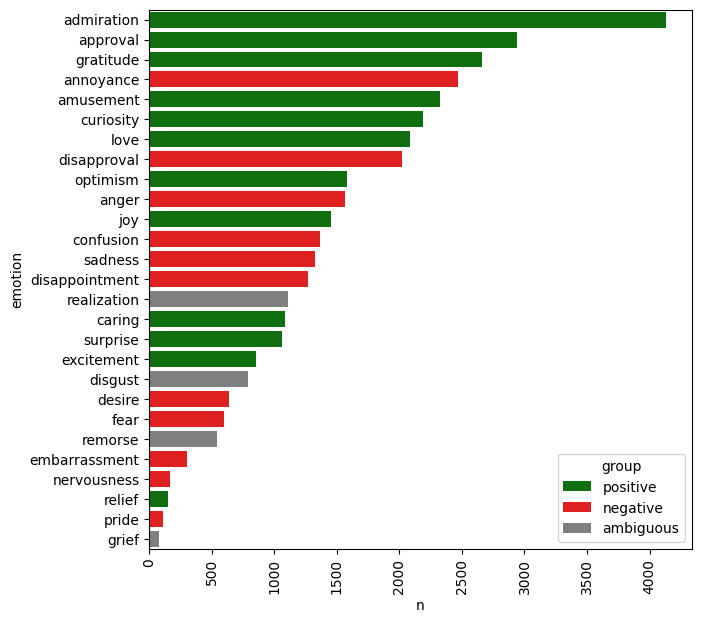
\includegraphics[width=0.8\textwidth]{figures/image24}
  \caption{Emotion distribution \cite{ref77}}
  \label{fig:ch4_f2}
\end{figure}

\section{Federated Framework Implementation}
This section describes how PRADO is used to build a federated learning framework that improves recommendation performance across domains (Emotions $\rightarrow$ Books, Emotions $\rightarrow$ Movies, Emotions $\rightarrow$ Songs, Emotions $\rightarrow$ Games). Despite the limited resources on client devices, PRADO manages on-device training efficiently. Identifying semantically similar terms is vital in this study, as it enhances recommendations across source and target domains. The trainable projection Model effectively captures long-range word dependencies and is proficient at categorizing lengthy texts.

All experiments in this research work are run on an Apple M4 Max (128 GB unified memory), GPU via Metal (tensorflow-metal 1.1.0), Python 3.11 with TensorFlow 2.15.1/Keras 2 and scikit-learn 1.9. Every notebook executes top-to-bottom under papermill on the seq-flow-lite-metal kernel. The aggregation server (MLServer; Spring Boot/Kotlin) runs on http://localhost:8080 and exposes setParamSeqFlow, getParamAvgSeqFlow, resetFedAvg, and fedAvgStatus with an aggregation buffer of 120. Section 4.5.1 provides an overview and notations used during implementation. Section 4.5.2 \& 4.5.3 elaborate federated training on the emotion model and the server aggregation process in depth, and Section 4.5.4 discusses the federated recommendation process.

\subsection{Overview and Notations}
The system studies content-based recommendation in which the only learned component is a federated text model. Two federated emotion models are trained on GoEmotions with K = 120

simulated clients: a fully federated PRADO network and a federated classification head on a frozen Small-BERT encoder \cite{ref98}. Aggregation is performed server-side by a Spring Boot service (MLServer) implementing streaming, buffered/weighted FedAvg (4.5.3).

Each target item $t_{i}$ (a movie, song, game, or book) is represented by a set of short text chunks $C_{i} = \{c_{1}, c_{2}, \ldots, c_{|C_{i}|}\}$ (plot sentences, four-line lyric stanzas, store-page sentences, or reviews). The end-to-end pipeline for one target item is:

\begin{equation}
  t_{i} \xrightarrow{\text{chunk}} C_{i} \xrightarrow{\text{fingerprint}} \{\phi(c) : c \in C_{i}\} \xrightarrow{\text{profile}} P_{i} \xrightarrow{\text{rank}} \text{score}(q, t_{i})
  \label{eq:ch4_pipeline}
\end{equation}

\noindent In this pipeline flow,

\begin{itemize}
    \item $t_{i}$ represents one target item: a movie, song, game, or book that can be recommended.
    \item $C_{i}$ represents the set of short text chunks describing the item: plot sentences, four-line lyric stanzas, store-page sentences, or reviews.
    \item $|C_{i}|$ is the number of chunks the item has.
    \item $c$ represents a single chunk (one short text) drawn from $C_{i}$.
    \item $\phi(c)$ represents the emotion fingerprint of chunk $c$: 27 numbers in $\mathbb{R}^{27}$, one per GoEmotions emotion (neutral is dropped), produced by a federated global model (Sec. 4).
    \item $e(c)$ represents the penultimate embedding: the federated PRADO model's 128-dimensional internal activation immediately before its output layer (Sec. 6). The 28 emotion scores are one linear function of $e(c)$, so $e(c)$ carries strictly more information than $\phi(c)$.
    \item $\mathbb{R}^{27}$ is the set of real-valued vectors with 27 components; writing $\phi(c) \in \mathbb{R}^{27}$ says that a fingerprint is a list of 27 real numbers.
    \item $|C_{i}|$ denotes target size and $\text{rank}(q)$ the rank of the query $q$'s target item under a given scorer.
\end{itemize}

denotes target size and  the rank of the query ’s target item under a given scorer.
In simple words, the end-to-end pipeline indicates that every item is broken into short texts; the federated model maps each short text to either a 27-emotion profile or a 128-number internal embedding; those vectors are then combined to represent, query, and rank items.

\subsection{Federated training of the emotion models}
Model training in the FL environment occurs on the local device with the distributed data, as mentioned in Section 3.3. The algorithm 1 demonstrates the key steps followed for training the model on the client-side using PRADO.

\begin{algorithm}[htbp]
\caption{Federated PRADO training (multi-round FedAvg). Takes the GoEmotions dataset as input. Data is divided among 120 clients. The model is trained for 20 communication rounds. During each round, 20 local training steps (epochs) are performed, with a batch size of 256, a learning rate of 0.5, and a momentum of 0.9. The weights are initialized to 5. The learning rate is scheduled using cosine decay (Eq.~\ref{eq:ch4_4_5}). Each client performs training on its own data using mini-batches. The weight $W$ at round $r$, $W_r$, at each internal training round is reset to zero to ensure every communication round starts with the same optimization settings. It updates the model parameters and minimizes the weighted binary cross-entropy loss (Eq.~\ref{eq:ch4_4_3}). The update process includes optimization using SGD (Eq.~\ref{eq:ch4_4_4}). After local training, the updated client models are sent back to the server, where they are aggregated using weighted Federated Averaging (Eq.~\ref{eq:ch4_4_6}) based on the number of local training samples. The aggregated model becomes the new global model and is redistributed for the next communication round. This iterative process continues until all communication rounds are completed, resulting in the final global PRADO model while preserving data privacy by keeping the training data on client devices.}
\label{alg:ch4_alg1}
\begin{algorithmic}[1]
\Require GoEmotions training set $\mathcal{D}$ (43,410 examples); clients $K=120$; rounds $R=20$; local steps $T=20$; batch $B=256$; peak rate $\eta=0.5$; momentum $0.9$; weight $w_d=5$
\Ensure global weights $W^*_R$; the final round's $K$ client models
\State Partition $\mathcal{D}$ into $K$ iid shards $\mathcal{D}_1,\ldots,\mathcal{D}_K$ by a seeded permutation (seed 42); persist the split
\State $W_0 \leftarrow$ a single shared random initialisation
\For{$r=0,\ldots,R-1$}
    \State $\eta_r \leftarrow \frac{\eta}{2}(1+\cos\frac{r\pi}{R})$ \hfill // cosine decay of Eq.~\ref{eq:ch4_4_5}
    \For{$k=1,\ldots,K$}
        \State \textbf{repeat}
        \State \quad load $W_r$; reset all optimiser state
        \State \quad run $T$ steps of the update of Eq.~\ref{eq:ch4_4_4} on $\mathcal{D}_k$, minimising Eq.~\ref{eq:ch4_4_3}
        \State \quad $W_{r,k} \leftarrow$ resulting weights; $m_{r,k} \leftarrow |\mathcal{D}_k|$
        \State \textbf{until} convergence
    \EndFor
    \State $W_{r+1} \leftarrow$ Eq.~\ref{eq:ch4_4_6}
\EndFor
\State persist $W^*_R$ as the client checkpoints uploaded in Algorithm~\ref{alg:ch4_alg2}
\end{algorithmic}
\end{algorithm}

\subsubsection{Model Output}
For an input text, the PRADO network produces one logit  per GoEmotions label, converted to an independent probability by the logistic sigmoid using equation (4.2):

\begin{equation}
  p_{l} = \sigma(z_{l}) = \frac{1}{1 + e^{-z_{l}}}, \quad l = 1, \ldots, 28
  \label{eq:ch4_4_2}
\end{equation}

$l$ --- the label index; GoEmotions has 28 emotion labels (27 emotions plus neutral).

$z_{l}$ --- the raw, unbounded score (logit) the network’s last linear layer assigns to label $l$.

$\sigma(\cdot)$ --- the logistic sigmoid function; it squashes any real number into the interval $[0,1]$.

$p_{l}$ --- the model’s predicted probability that the text expresses emotion $l$.

In simple words, equation (4.2) indicates each emotion gets its own independent yes/no probability. A sigmoid per label (rather than a softmax across labels) is what makes the problem multilabel: a text may be both “joy” and “surprise” at once, so the 28 probabilities need not sum to one.

\subsubsection{Minimize Client Loss}
The input dataset for PRADO is GoEmotions. The distribution of emotion frequency in dataset is shown in Figure 4.3. It indicates that there is majorable difference in number of samples of every emotiion. This affect on client’s performance. To minimize client loss, a positive-class--weighted binary cross-entropy (BCE) over the 28 labels is applied using equation (4.3):

\begin{equation}
  \mathcal{L}(y, p) = -\frac{1}{28} \sum_{l=1}^{28} \left[ w_{+} y_{l} \log p_{l} + (1 - y_{l}) \log(1 - p_{l}) \right], \quad w_{+} = 5
  \label{eq:ch4_4_3}
\end{equation}

$\mathcal{L}$ --- the loss (training penalty); smaller is better; training adjusts weights to reduce it.

$\mathbf{y}$ --- the ground-truth label vector; $y_{l} \in \{0, 1\}$ indicates whether emotion $l$ is truly present ($1$) or absent ($0$) in the example.

$\mathbf{p}$ --- the predicted probabilities from Eq. (4.2).

$\log(\cdot)$ --- the natural logarithm; $-\log(p)$ grows without bound as $p \to 0$, so confident mistakes are punished heavily.

$w_{+}$ --- the positive-class weight: the penalty for missing a present emotion is multiplied by 5.

$\frac{1}{28}$ --- the average over all 28 labels, so the loss scale does not depend on the label count.

For each label, the model pays a penalty  if the emotion is present (large penalty for assigning it low probability) and  if it is absent (large penalty for assigning it high probability); finally, the 28 penalties are averaged. The penalty applied (  ) is an essential component of more than just adjustment. As most emotion labels in the GOEmotions dataset occur infrequently, training with equal class weights (w sub plus equals 1) causes the model to favor predicting the absence of that emotion. In such cases, the large number of negative samples dominates the loss function, and the model achieves low recall for minority emotion classes. The penalty applied helps the model learn minority emotions more effectively. This results in balanced precision and recall.

\subsubsection{Optimization at Local Device}
During the first stage of experimentation, the Adam optimizer was used to optimize the client’s performance. However, it showed that this optimizer creates client-specific updates that prevented successful aggregation in federated learning. This prevents the global model from learning meaningful representations. Hence, in updated experimentation, each client runs Stochastic gradient descent (SGD) with momentum on its shard as given in equation (4.4).

\begin{equation}
  v \leftarrow 0.9v - \eta_{r} \nabla_{W} \mathcal{L}_{\mathcal{B}}(W), \quad W \leftarrow W + v
  \label{eq:ch4_4_4}
\end{equation}

$W$ --- the client’s current model weights (all trainable parameters, treated as one long vector).

$\nabla_{W} \mathcal{L}_{\mathcal{B}}(W)$ --- the gradient of the loss of Eq. (4.3), averaged over one mini-batch $\mathcal{B}$ ($|\mathcal{B}| = 256$).

$v$ --- the momentum (velocity) buffer, initialized to zero at the start of every round; it accumulates an exponentially decaying average of past gradients.

$0.9$ --- the momentum coefficient: 90\% of the previous velocity is retained each step, smoothing the descent direction.

$\eta_{r}$ --- the learning rate in round $r$ (Eq. (4.5) below): the step size.

The experimental footprints of the revised optimizer are discussed below.

\subsubsection{Scheduling Learning rate}
At early rounds of model training, the model requires large steps to make fast progress, and later it takes tiny steps. So the 120 clients stay close to the shared starting point and average cleanly. For a particular round, all clients use the same.  .  The learning rate is decayed across communication rounds by a cosine schedule.

\begin{equation}
  \eta_{r} = \frac{1}{2} \eta \left(1 + \cos \frac{\pi r}{R-1}\right), \quad r = 0, \ldots, R-1, \quad \eta = 0.5
  \label{eq:ch4_4_5}
\end{equation}

$\eta$ --- the peak learning rate, used in the first round.

$r$ --- the round index, running from $0$ to $R-1$.

$R$ --- the total number of communication rounds.

$\cos\frac{\pi r}{R-1}$ --- moves smoothly from $1$ (first round) to $-1$ (last round), so $\eta_{r}$ moves smoothly from $\eta$ down to $0$.

\subsubsection{Updated Server Aggregation}
The aggregation process demonstrated in equation (4.1) is updated as per the implementation requirement of the proposed model. The global model is updated using a weighted average (FedAvg) of the client models.

\begin{equation}
  W_{r+1} = \sum_{k=1}^{K} \frac{n_{k}}{n} W_{r}^{k}, \quad n = \sum_{k=1}^{K} n_{k}
  \label{eq:ch4_4_6}
\end{equation}

$K$ --- the number of clients: simulated parties, each holding a private data shard that never leaves it.

$W_{r}^{k}$ --- client $k$’s weights after its local training in round $r$ (each client started the round from the same global $W_{r}$).

$n_{k}$ --- the number of training examples on client $k$ (here 361--362).

$n$ --- the total number of examples across all clients (43,410).

$\frac{n_{k}}{n}$ --- client $k$’s mixing weight: clients with more data count proportionally more. The weights sum to 1, so the result is a convex combination.

$W_{r+1}$ --- the new global model broadcast at the start of the next round.

As demonstrated in the last step of Algorithm 1, the client’s weights are uploaded to the server. They are further processed according to the Server-side aggregation protocol.

\subsection{Server-side aggregation protocol}
MLServer (server-Spring Boot service) maintains a running weighted sum $S$, a sample total $n$, an upload counter $c$, and the last computed average $A$. Uploads are JSON weight sets with the client’s shard size. On each upload $(w, n_k)$ the server performs the streaming update

\begin{equation}
  S \leftarrow S + n_{k} \cdot \text{flatten}(w), \quad n \leftarrow n + n_{k}, \quad c \leftarrow c + 1
  \label{eq:ch4_4_7}
\end{equation}

$w$ --- one client’s uploaded weights (a structured set of arrays).

$\text{flatten}(w)$ --- those arrays concatenated into one long vector, so the server does arithmetic on a single vector regardless of the model’s layer structure.

$S$ --- the running weighted sum of all flattened uploads so far. Only this one vector is stored --- never the 120 individual uploads.

$n$ --- the running total of shard sizes; $c$ --- how many clients have uploaded in the current round.  Equation (4.7) indicates that each upload is folded into a single accumulator vector and then discarded. Memory cost is of only one model, not 120. When the counter reaches the buffer size ($c = 120$) the average is computed asynchronously, in a background coroutine:

\begin{equation}
  A \leftarrow \text{unflatten}(S/n), \quad S \leftarrow n \cdot \text{flatten}(A), \quad c \leftarrow 0
  \label{eq:ch4_4_8}
\end{equation}

$A$ --- the sample-weighted mean of Eq. (4.6), computed in flattened form; restores the original layer structure.

$A$ --- the last computed global average, served by GET /getParamAvg (HTTP 409 ``Conflict'' if none exists yet).

$c$ --- re-seeding: the accumulator is reset to "$S \leftarrow n \cdot \text{flatten}(A)$", weighted by all $n$ samples seen, so the next round's uploads blend with the current global model rather than starting from zero.

Averaging runs as a coroutine; the 120th upload’s HTTP response returns before the average exists. Clients must poll /fedAvgStatus until $c$ has returned to $0$ before fetching $A$, or risk reading a stale result of HTTP 409. The complete process is described stepwise in Algorithm2.

In Algorithm 2, $m$ represents the method an endpoint refers to: $w$ seqFlowLite (PRADO), $W$ represents the fetched global weights; $S$ represents the running sum; validation (line 1) represents that every upload’s array shapes, element types, and finiteness (no NaN/Inf) are checked against the round’s first upload, so one malformed client cannot silently corrupt $W_r$.

\begin{algorithm}[htbp]
\caption{Streaming weighted FedAvg on MLServer, and the client protocol. All locally trained model parameters, uploaded by clients, are first validated by the server to ensure consistency. The next step performs a streaming update (Eq.~\ref{eq:ch4_4_9}), i.e., received model weights are added to the aggregation buffer. This process continues until updates for all clients are received. Once updates from all clients are received, the buffered FedAvg is performed to generate new global weights.}
\label{alg:ch4_alg2}
\begin{algorithmic}[1]
\State \textbf{Server, on} \texttt{POST /setParam($m$)} with $(w, n_x)$:
\State \quad validate leaf types, finiteness, and weight count against the round's first client
\State \quad apply the streaming update of Eq.~\ref{eq:ch4_4_9}
\If{$c = 120$} \hfill // asynchronously, in a coroutine
\State \quad apply the averaging step of Eq.~\ref{eq:ch4_4_10} \hfill // $A$ seeds the next round
\EndIf
\State \textbf{Server, on} \texttt{POST /resetFedAvg}: $S, n, c \leftarrow 0$ ($A$ remains readable)
\State \textbf{Server, on} \texttt{GET /getParamAvg($m$)}: return $A$ (HTTP 409 if absent)
\State \textbf{Client upload procedure} (\texttt{ensure\_global\_weights}):
\If{GET /getParamAvg succeeds}
\State \quad use $A$ (fast path)
\Else
\State \quad \texttt{POST /resetFedAvg}; upload the 120 checkpoints with shard sizes
\State \quad poll \texttt{/fedAvgStatus} until $c = 0$ \hfill // averaging is asynchronous
\State \quad $W_{\text{glob}} \leftarrow$ GET \texttt{/getParamAvg}
\EndIf
\end{algorithmic}
\end{algorithm}

The third part of this process includes fingerprint extraction with a federated global model given in Algorithm 3.

\begin{algorithm}[htbp]
\caption{Fingerprint extraction with a federated global model. The emotion fingerprint is a fixed-length vector containing the predicted probabilities of all emotion classes (excluding the neutral class). It is a compact emotional representation of a text and is used for subsequent recommendation and similarity computations.}
\label{alg:ch4_alg3}
\begin{algorithmic}[1]
\Require text $t$; federated global model (PRADO or BERT head) from Algorithm~\ref{alg:ch4_alg2}
\State normalise whitespace in $t$
\If{model is PRADO FL}
\State $p \leftarrow \text{PRADO}_{\text{FedAvg}}(t)$ \hfill // raw string in; 28 sigmoid scores out
\Else
\State ids $\leftarrow$ WordPiece($t$), length 40; $x \leftarrow$ masked mean (Eq.~\ref{eq:ch4_4_7})
\State $p \leftarrow \text{head}_{\text{FedAvg}}(x)$
\EndIf
\Return $\phi(t) = p_{1:27}$ \hfill // label 28, neutral, is dropped
\end{algorithmic}
\end{algorithm}

\begin{equation}
  \phi(t) = (p_{1}, \ldots, p_{27}) = p_{1:27}, \quad p = \begin{cases} \text{PRADO}_{\text{FedAvg}}(t) & (\text{PRADO path}) \\ \text{head}_{\text{FedAvg}}(x_{t}) & (\text{BERT path}) \end{cases}
  \label{eq:ch4_4_9}
\end{equation}

--- the federated PRADO model applied to the raw string  (PRADO tokenizes internally); output is the 28 sigmoid scores of Eq. (4.2),  --- the first 27 of the 28 scores: label 28, neutral, is dropped.

\subsection{Federated Recommendation Process}
In sections 4.5.2 \& 4.5.3, a detailed discussion of federated emotion extraction and its server aggregation process is given. The recommendation process is implemented and assessed across three methods: the first using a Random Forest classifier, the second using 28-emotion probable output from PRADO (Featured Recommender Version1-V1), and the third using the model’s 128-dimensional penultimate representation (Featured Recommender Version2-V2). These implementations also provide their contribution to the final performance of the proposed model.

\subsubsection{Random-forest fingerprint lookup}
In case a random forest classifier is used in the original form, with a fixed decision tree, random-threshold splits, and no bootstrapping, its behavior is explained here. The input of the classifier is the emotion fingerprint of a review, and the output is the name of the book that this review belongs to. The model is trained on 10,000 sampled reviews, which correspond to 9,970 different book titles, so that almost all titles have only one book review. In recommendation, the model calculates the probability scores returned by predict\_proba($\phi(t)$) for candidate books and recommends the top-n books. The model simulates the original notebook's high accuracy of 99.54\% when performing the evaluation task in the original notebook's style using the proposed federated emotion fingerprints.

However, this high accuracy does not indicate that the recommender generalizes well to unseen data. Its performance is fundamentally limited by the following structural ceiling:

\begin{equation}
  \text{ceiling} = \frac{\left| \{ q \in D_{\text{test}} : \text{title}(q) \in \mathcal{Y}_{\text{train}} \} \right|}{|D_{\text{test}}|} = 0.40\%
  \label{eq:ch4_4_10}
\end{equation}

• $D_{\text{test}}$ --- the held-out 20\% of reviews under an 80/20 split; $\text{title}(q)$ --- the true book title of a test review $q$.

• $Y_{\text{train}}$ --- the set of titles that appear in the training data, i.e. the classifier’s label space.

• ceiling --- the fraction of test queries whose correct answer the classifier is even able to output. No classifier of this design can exceed it.

In this dataset, almost all book titles are unique. Once the data is split, the review of a specific book will usually be in the training set or the test set but not both. As a result, the proportion of the test reviews that match a classifier's previous classification is 0.40\%. To be precise, for the remaining 99.60\% of test titles, no classifiers will be able to predict the label, even if the classifiers are well trained.

Thus, the held-out accuracy observed is just 0.20\%, about half of the theoretical (0.40\%) accuracy. This indicates that the Random Forest focuses on the mapping between an emotion fingerprint and a book title, not on learning patterns that apply to unknown books.

\subsubsection{Featured Recommender Version1 (v1)}
The emotion classification model produces a 27-dimensional emotion fingerprint for each text chunk. This section describes how to generate recommendations and evaluate them. The main objective is to recommend the correct target item (book, song, movie, game, etc.) based on its emotional characteristics rather than memorizing titles. Below is a step-by-step explanation.

\subsubsection{Step 1: Build an item’s emotional profile (Eq.4.11)}
The chunks may contain multiple views; the mean of all these chunks is calculated using equation (4.11) and mapped over 27 emotions.

\begin{equation}
  P_{i} = \frac{1}{|C_{i}|} \sum_{c \in C_{i}} \phi(c) \in \mathbb{R}^{27}
  \label{eq:ch4_4_11}
\end{equation}

• $P_i$ --- item $i$'s emotion profile: mean fingerprint of all its chunks.

• $\frac{1}{|C_i|} \sum_{c \in C_i}$ --- arithmetic mean over item's chunk set.

\subsubsection{Step 2: Standardisation of  each emotion dimension (Eq.4.12)}
The review text may have different emotions at different scales. For example, a sentence may contain emotions related to joy, gratitude, anger, and fear, with a higher average score for joy; if cosine similarity is computed directly, it may dominate the selection of the correct target item. To solve this problem, every emotion dimension is converted to z-score using Eq.(4.12)

\begin{equation}
  \begin{aligned}
  z(v)_{d} &= \frac{v_{d} - \mu_{d}}{\sigma_{d}}, \\
  \mu_{d} &= \frac{1}{N} \sum_{i=1}^{N} (P_{i})_{d}, \\
  \sigma_{d}^{2} &= \frac{1}{N} \sum_{i=1}^{N} \left( (P_{i})_{d} - \mu_{d} \right)^{2}
  \end{aligned}
  \label{eq:ch4_4_12}
\end{equation}

• $v_d$ --- the $d$-th component ($d=1,\ldots,27$) of fingerprint vector $v$.

• $\mu_d$, $\sigma_d$ --- mean and std. of dimension $d$ over all $N$ target item profiles.

• $z(v)$ --- the standardized vector: every dimension now has zero mean and unit variance across the target items.

Step 3: Compare the item’s standardized emotional profile with the user query Eq. 4.13)

\subsubsection{Step 3: Compare the item's standardized emotional profile with the user query (Eq. 4.13)}
The standardized emotional profile is compared with the user query using Equation (4.13). Items are ranked by cosine similarity of the standardized vectors. Cosine similarity itself is

\begin{equation}
  \cos(a, b) = \frac{a \cdot b}{\|a\| \, \|b\|} = \frac{\sum_{d} a_{d} b_{d}}{\sqrt{\sum_{d} a_{d}^{2}} \, \sqrt{\sum_{d} b_{d}^{2}}} \in [-1, 1]
  \label{eq:ch4_4_13}
\end{equation}

• $a \cdot b$ --- the dot product of the two vectors; $\|a\|$ --- the Euclidean length of $a$.

• $\cos(a, b)$ --- the cosine of the angle between $a$ and $b$: $1$ for identical directions, $0$ for unrelated (orthogonal) ones, $-1$ for opposite ones. It ignores vector magnitude entirely, and the v1 ranking score is

Each emotion profile is an arrow in a 27-dimensional vector. Cosine similarity measures the angle between the two arrows. It returns 1 if the emotional patterns are the same or 0 if the emotional patterns are opposite.

\subsubsection{Step 4: Recommendation score computation (Eq. 4.14)}
The recommendation score is computed using Eq. 4.12 and 4.13. Eq. (4.14) shows the combined version for computing it.

\begin{equation}
  s(q, i) = \cos\left( z(\phi(q)), \, z(P_{i}) \right)
  \label{eq:ch4_4_14}
\end{equation}

• $q$ --- the query: a single held-out chunk; $\phi(q)$ emotions fingerprint (Eq. (4.11)).

• $z(\cdot)$ --- the target item's standardization of Eq. (4.12), applied to both sides.

• $s(q, i)$ --- the score by which all $N$ items are sorted (descending) to produce the recommendation list for $q$.

Duplicate-chunk guardrail.

In all corpora, duplicate chunks (after normalizing text) are eliminated within the items. This is not a preference, but a correctness requirement: Amazon presents the same review text as multiple review editions (37\% of the number of rows in the multi-review table), and song choruses repeat ($\sim$6\% of the number of rows in the table of stanzas); with duplicates in place, held-out ``retrieval'' becomes duplicate matching, and the median rank is 1 (before fix).

\subsubsection{Hold-one-out evaluation}
For each $|C_i| \ge 2$, one chunk is held out (seed 42): all profiles are rebuilt without the held-out chunks; each held-out chunk queries the whole catalog: the rank of its own item feeds the metrics of Sec. 7 (at most 3,000 queries). The difficulty in rebuilding the profiles without the chunk shown makes evaluation fair: the query text doesn't ''push'' into the profile it's trying to build.

\subsubsection{Featured recommender Version2(v2)}
The second version of the recommendation system(V2) is discussed in this section. This system does not retrain the Federated PRADO. It uses the model weights from Section 4.5.2. It combines three complementary similarity views to capture different information about the target item. The following three changes convert the same federated PRADO model into a substantially stronger retriever. (i) Instead of probable emotion, retrieval uses the model’s 128-dimensional penultimate representation  (the concatenated attention-pooled bigram and trigram channels). The emotion scores are a single linear readout:  with . Working with  retains everything the federation learned about the text, not only its projection onto 28 emotions.

(ii) Document queries. For every item with , a random half  forms the query document and the complement  the profile. The split precedes any windowing, so no text occurs on both sides; the ranked target item is always the full one.

(iii) Ensemble scorer. Embedding centroids are first PCA whitened. The whitening transformation first centres the data, then rotates it into principal directions and then scales every direction to unit variance. Equation (4.15) gives the whitening transform, fitted on the  profile centroids (respectively on a 60k-chunk sample for ), is

\begin{equation}
  \begin{aligned}
  \Psi(x) &= \text{diag}\!\left( \frac{s_{j}}{\sqrt{n-1}} + \varepsilon \right)^{-1} V^{\top}(x - \mu) \\
  \widetilde{X} &= X - \mathbf{1}\mu^{\top} = U \, \text{diag}(s) \, V^{\top}
  \end{aligned}
  \label{eq:ch4_4_15}
\end{equation}

• $X$ --- the matrix whose rows are the fitting vectors (profile centroids, or the 60k chunk embeddings); $n$ --- the number of rows; $\mu$ --- their mean vector, subtracted from every row.

• $X = U \, \text{diag}(s) \, V^\top$ --- the singular value decomposition of the centred matrix: $V$'s columns are the principal directions (axes of greatest variance), and the singular values $s_j$ measure the data's spread along each.

• $V^\top(x - \mu)$ --- centre the input and rotate it into the principal-axis coordinate system.

• $\text{diag}(s_j / \sqrt{n-1} + \varepsilon)^{-1}$ --- divide each rotated coordinate by that axis's standard deviation, so every axis has unit variance after the transform.

• $\varepsilon = 10^{-6}$ --- a numerical floor preventing division by near-zero singular values on nearly flat directions.

• $\Psi(x)$ --- the whitened vector.

Whitening makes cosine similarity focus on meaningful differences instead of common characteristics like writing style, sentence length, common vocabulary, etc. (for books as the target item). If cosine similarity is applied directly/ then the common characteristics create bias in recommendation. The extension of three changes is described as 3 views.

View 1: Centroid Cosine(whitened):- chunk embeddings from each document half are averaged into one vector. E.g. chunk1,chunk2,chunk3  Average  Centroid. The cosine similarity between the query and candidate centroid is computed. It captures the general topic of the document.

\begin{equation}
  \begin{aligned}
  S_{1}(q, i) &= \cos\!\left( \Psi\!\left( \overline{e}(Q_{q}) \right), \, \Psi\!\left( \overline{e}(P_{i}) \right) \right) \\
  \overline{e}(X) &= \frac{1}{|X|} \sum_{c \in X} e(c)
  \end{aligned}
  \label{eq:ch4_4_16}
\end{equation}

• $Q_q$ --- the query half of the querying item's chunks; $P_i$ --- the profile half of the candidate item $i$'s chunks.

• $\overline{e}(X)$ --- the centroid: the mean of the embeddings of the chunk set $X$; one 128-dimensional summary vector per side.

• $S_1(q, i)$ --- whitened-centroid cosine: how similar the query document's average embedding is to the candidate's average embedding.

View 2: It repeats view1 for neighboring sentences, i.e., a 2-chunk window. It helps to capture the relationship among neighboring sentences, context, and narrative flow, given by Eq.(4.17)

\begin{equation}
  S_{2}(q, i) = S_{1}, \text{ but with } e(\cdot) \text{ applied to 2-chunk windows formed inside each half}
  \label{eq:ch4_4_17}
\end{equation}

• 2-chunk window --- two consecutive chunks of one half concatenated and embedded as a single text, giving the model slightly longer context than a lone sentence or stanza.

• “inside each half” --- windows never span the query/profile boundary, preserving the leak-free split of design choice (ii).

View 3: It is a late interaction score: there is no pooling of summaries; each query sentence searches the candidate for the matching sentence. It rewards items that match specific sentences rather than the overall blend, complementing the centroid views given by Eq.(4.17)

\begin{equation}
  S_{3}(q, i) = \frac{1}{|Q_{q}|} \sum_{c \in Q_{q}} \max_{c' \in P_{i}} \cos\left( \Psi(e(c)), \, \Psi(e(c')) \right)
  \label{eq:ch4_4_18}
\end{equation}

• $c$ --- one individual query chunk; $c'$ --- one individual profile chunk of the candidate $i$.

• $\max_{c' \in P_i}$ --- each query chunk's similarity to its single best-matching profile chunk of the candidate.

• $\frac{1}{|Q_q|} \sum_{c \in Q_q}$ --- the query's chunks then vote by averaging their best-match scores.

\subsubsection{Standardizing the view scores}
These similarity views produce scores on different scales, like 0.91, 15, or 0.25. Hence, before fusing, each view’s score row is standardized per query using Eq.(4.18)

\begin{equation}
  \zeta(S)_{q,i} = \frac{S(q, i) - \text{mean}_{i'} \, S(q, i')}{\text{std}_{i'} \, S(q, i')}
  \label{eq:ch4_4_18_dup}
\end{equation}

• $\text{mean}_{i'}$, $\text{std}_{i'$} --- mean and standard deviation taken over all $N$ candidate items for the same query $q$ (i.e. across one row of the score matrix).

• $\zeta(S)_{q,i}$ --- item $i$'s score re-expressed The final ensemble score is the weighted sum

\begin{equation}
  S(q, \cdot) = w_{1} \, \zeta(S_{1}) + w_{2} \, \zeta(S_{2}) + w_{3} \, \zeta(S_{3})
  \label{eq:ch4_4_19}
\end{equation}

• $w_1, w_2, w_3$ --- non-negative per-domain fusion weights, tuned on a seed-42 grid: movies $(0.3/0.2/0.5)$, music $(0.4/0.0/0.6)$, games $(0.25/0.15/0.6)$, books $(0.35/0.1/0.55)$.

• $S(q, \cdot)$ --- the fused score of every target item for the query $q$; items are ranked by it in descending order.

The v2 retrieval framework boosts recommendation accuracy without the need to retrain the federated model PRADO. Instead, it provides more enriched embeddings, a more leakage-free document-splitting strategy, PCA-based whitening, and a three-view ensemble ranking method using the learned representations. The 128-dimensional embeddings contain significantly more meaning than the final emotion probabilities, and the split-half evaluation guarantees unbiased evaluation. Whitening is used to remove uninformative embedding directions that dominate the embedding, and the ensemble consists of document-level summaries, contextual windows, and sentence-level matching, all with a combined ranking score. These enhancements can be used together to enable the recommender to retrieve items by deeper semantic and emotional similarity (meaning that they are not just remembered, but also understood), leading to a stronger and more generalizable recommendation system.

\begin{algorithm}[htbp]
\caption{PRADO FL v2: federated embeddings, split-half document queries, three-view ensemble.}
\label{alg:ch4_alg4}
\begin{algorithmic}[1]
\Require chunked catalogue $\{C_i\}$; federated PRADO weights (Algorithm~\ref{alg:ch4_alg2})
\State $e(c) \leftarrow$ penultimate PRADO activation for every chunk $c$
\State split each $C_i$ ($|C_i| \geq 4$) into query half $Q_i$ and profile half $P_i$ (seed 42), before any windowing
\State compute $S_1, S_2, S_3$ by Eqs.~\ref{eq:ch4_4_17}--\ref{eq:ch4_4_18} over the full catalogue
\State fuse by Eqs.~\ref{eq:ch4_4_19}--\ref{eq:ch4_4_19} with the domain's weights; rank items
\State evaluate with Sec.~7 (3,000 queries, seed 42)
\end{algorithmic}
\end{algorithm}

The complete process discussed in Section 4.5 is summarized in the following steps

\subsubsection{Pipeline (identical in every domain notebook):}
The FL global emotion model is fetched from MLServer (120-client weighted FedAvg; the saved client checkpoints are uploaded first if the server holds no average). PRADO consumes raw strings; BERT is the federated classifier head on top of the frozen Small BERT encoder (shared preprocessing).

Every item's text is split into GoEmotions-comment-sized chunks: plot sentences for Movies, review text for Books, 4-line lyric stanzas for Music, and store-page sentences for Games. Each chunk becomes a 27-dim emotion fingerprint (neutral dropped).

An item's emotional profile is the mean of its chunk fingerprints (multiple texts per item).

Recommender: Two versions of recommenders (V1 and V2) are implemented, using cosine similarity between z-scored profiles (z-scoring per emotion dimension across the catalog stops uniformly-loud dimensions from drowning rare, discriminative ones --- measured in the raw-vs-z ablation (Equations 4.15-4.19).

\subsubsection{Runtime details and reproducibility}
Uploading a full federated round takes 13 s (120 PRADO models) and 80 s (120 BERT heads); server averaging completes in seconds. Fingerprinting the largest corpus (movies, 255,602 chunks) takes 4 s with PRADO versus 297 s with BERT (68); the two v2 embedding views cost 6 s. Federated training itself takes 11 min (PRADO,  client fits) and 2 min (BERT heads); the recommendation suite reuses the persisted final-round checkpoints. All sampling, splits, and tuning grids derive from seed 42 and reproduce digit-for-digit; per-notebook JSON artifacts (metrics, ranks, timings) feed both companion documents, and a single shared module (fl\_common.py) implements every algorithm above.

\section{Performance Analysis}
This section outlines the performance analysis of the proposed advancements in basic Modular Federated CDR on emotion classification and cross-domain recommendation.

\subsection{Client Optimizer ablation (Equation 4.4)}
The revision of the training process is grounded in a controlled ablation over client optimizers and local-work budgets, run on identical shards from the identical initialization (fixed seed; every configuration is exactly reproducible). Adam clients --- the original choice --- leave the global model at chance level: their per-parameter adaptive scaling turns the 120 local updates into mutually incoherent directions whose average carries almost no signal. Replacing the client optimizer with SGD + momentum turns federated averaging constructive, and quality then scales with local work and learning rate: at lr 0.5 with 20 local steps the global model passes the best Adam variant within two rounds and reaches 0.20 test loss by round four. This single change explains the difference between the collapsed one-shot results and the revised process. The same mechanism, amplified by their dominant trainable embedding tables (2.56M of \textasciitilde{}2.7M parameters trained on \textasciitilde{}362 examples per client), is what destroys the one-shot federated LSTM and Bi-LSTM: each client's embedding rows co-adapt with its own recurrent gates, the 120 configurations are mutually incompatible, and their average passes no input signal --- the averaged network outputs each label's base rate for every input, hence deceptively low loss with zero precision and recall. BERT is insulated because its encoder is frozen and shared, leaving only a near-convex head to average.

\begin{figure}[htbp]
  \centering
  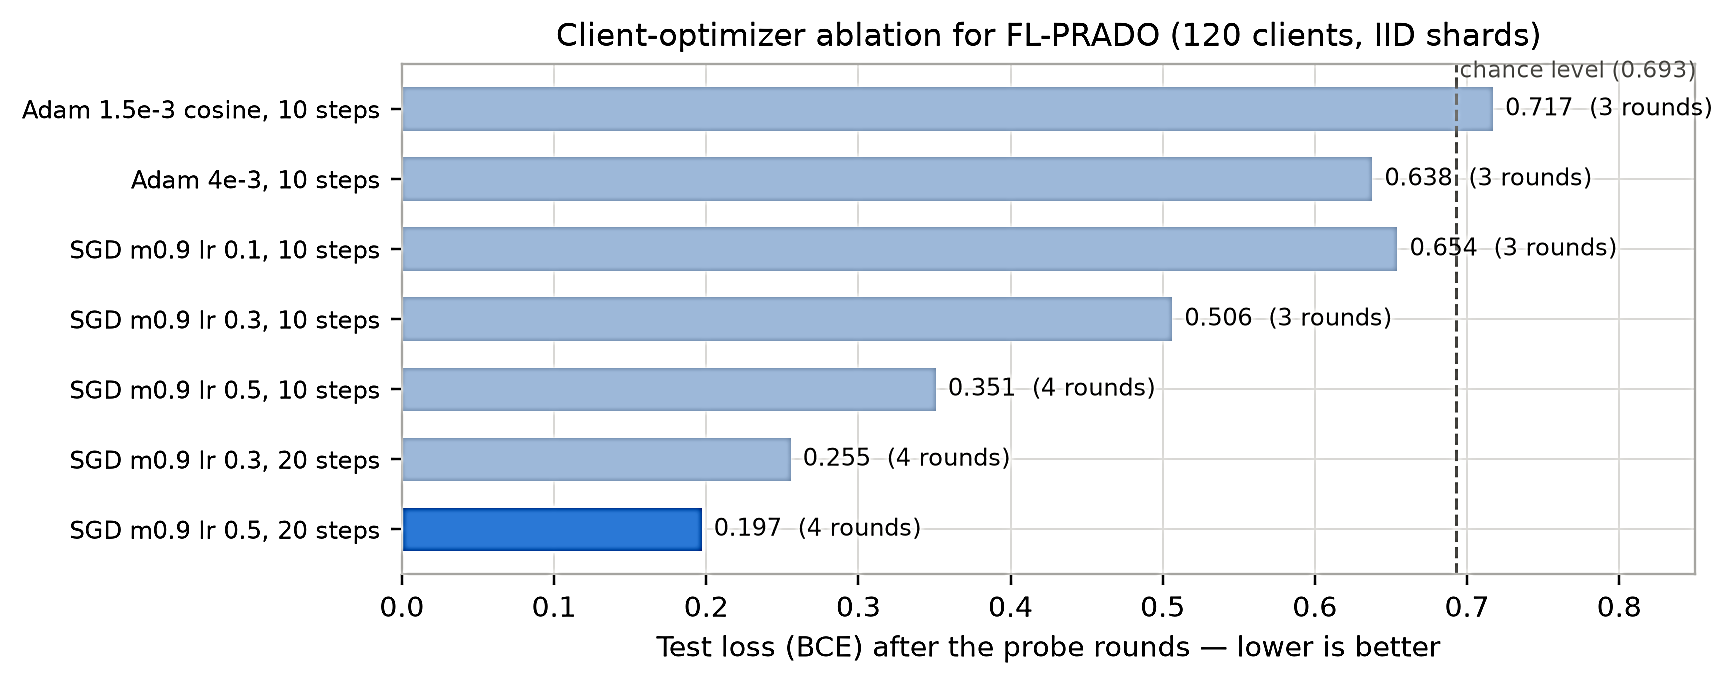
\includegraphics[width=0.8\textwidth]{figures/image29}
  \caption{Client-optimizer ablation: test loss of the FL-PRADO global model}
  \label{fig:ch4_f7}
\end{figure}

\subsection{Operating-Point Control: Positive-Class Weight}
\begin{longtable}{|c|c|c|c|c|}
\caption{Effect of positive weight class in client objective}
\label{tab:ch4_t2} \\
\hline
POS\_WEIGHT & Test Loss & Precision@5 & Recall@5 & F1-Score \\
\hline
\endfirsthead
\hline
POS\_WEIGHT & Test Loss & Precision@5 & Recall@5 & F1-Score \\
\hline
\endhead
\hline
\endfoot
1 & 0.157 & 0.724 & 0.098 & 0.172 \\
\hline
3 & 0.160 & 0.517 & 0.390 & 0.445 \\
\hline
5 & 0.174 & 0.469 & 0.477 & 0.473 \\
\hline
\end{longtable}

With the plain objective (weight 1) the federated model converges to an extremely conservative solution --- excellent precision but recall 0.10, and a threshold sweep shows its precision-recall curve cannot reach the centralized operating point at any threshold, so no post-hoc calibration can repair it. Weight 3 matches the centralized recall (0.39) at precision 0.52; weight 5 maximizes F1 at a balanced operating point and is the default of the revised process. Figure 4.6-K places the resulting model's full precision-recall trade-off next to the centralized PRADO operating point. The effect of positive weight class is listed in Table 4.6.1 and its graph is shown in Figure 4.6.2. Figure 4.6.3 shows the trade-off of the final FL-PRADO global model.

\clearpage
\begin{figure}[htbp]
  \centering
  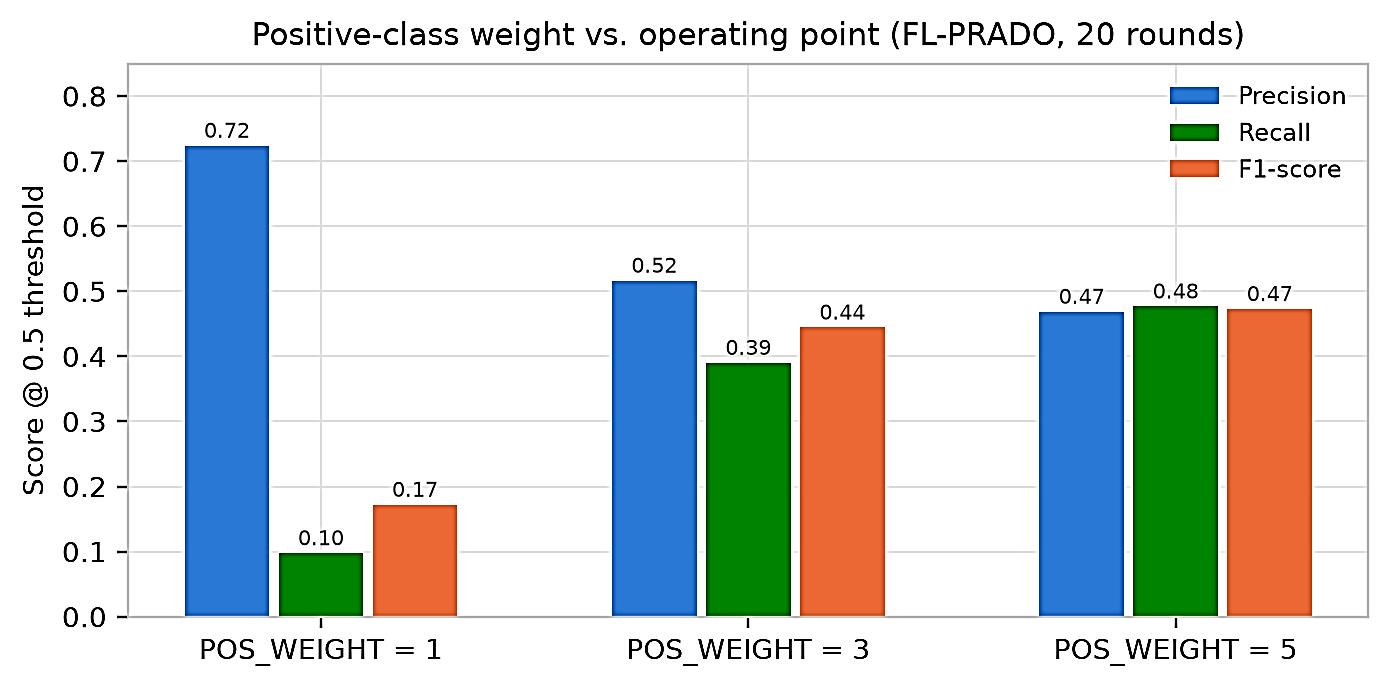
\includegraphics[width=0.8\textwidth]{figures/image30}
  \caption{Precision/recall/F1 at the 0.5 threshold as a function of the positive-class weight (FL-PRADO, 20 rounds)}
  \label{fig:ch4_f8}
\end{figure}

\begin{figure}[htbp]
  \centering
  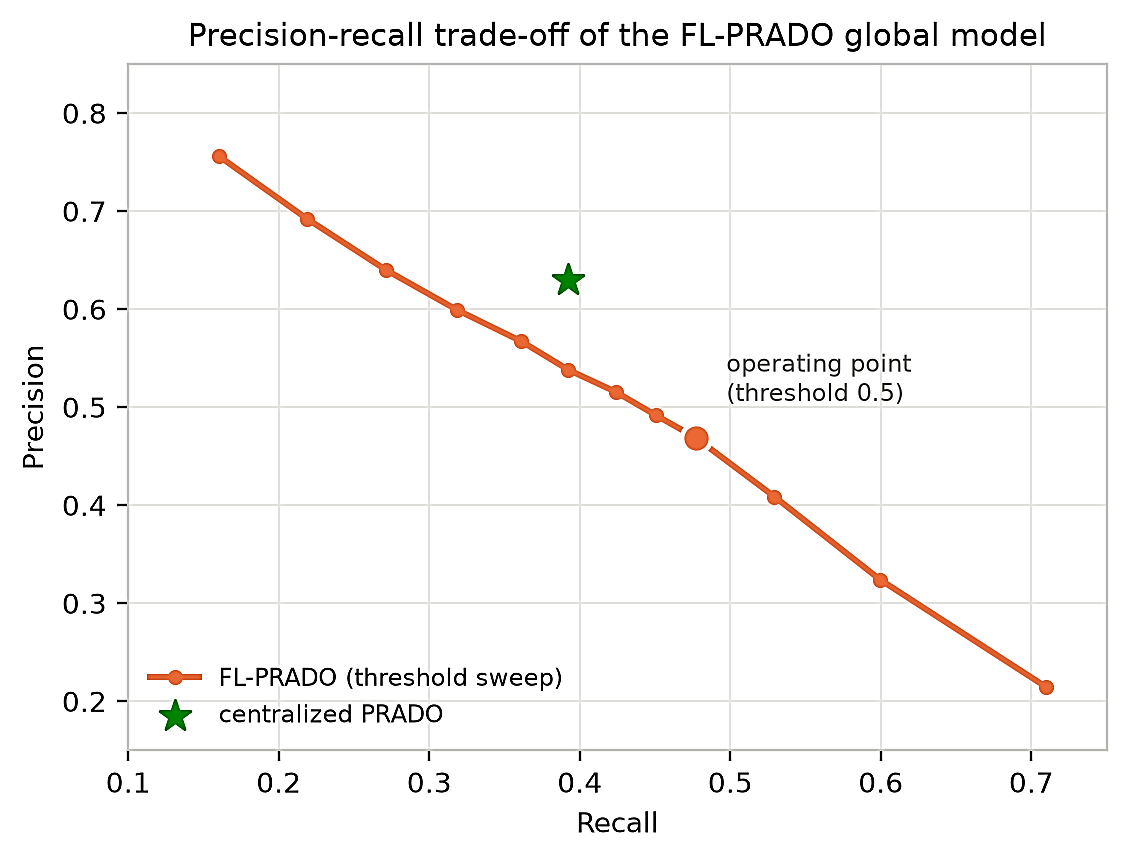
\includegraphics[width=0.8\textwidth]{figures/image31}
  \caption{Precision-recall trade-off of the final FL-PRADO global model}
  \label{fig:ch4_f9}
\end{figure}

The centralized PRADO reference point has higher precision and lower recall, and FL-PRADO has higher recall and acceptable precision. Overall, FL-PRADO is flexible, enabling a proper trade-off between prediction accuracy and coverage while maintaining the privacy of federated learning.

\subsection{Qualitative Results}
Table 4.3 presents the top-3 predicted emotions for the three reference prompts, generated by the federated PRADO model. The predictions from the local weighted-average model and the MLServer aggregation endpoint are nearly identical (matching to float32 precision). The revised federated PRADO reproduces the centralized top predictions with comparable confidence, and on ''I love you,'' its secondary predictions are arguably more sensible than the centralized model's spurious nervousness (0.989).

\begin{longtable}{|p{3cm}|p{3.5cm}|p{3.5cm}|p{3.5cm}|}
\caption{Comparative Confidence Score for Emotion Predictions across models}
\label{tab:ch4_t3} \\
\hline
\makecell{Input \\ text} & PRADO & \makecell{PRADO FL \\ (revised)} & \makecell{BERT FL \\ (one-shot)} \\
\hline
\endfirsthead
\hline
\makecell{Input \\ text} & PRADO & \makecell{PRADO FL \\ (revised)} & \makecell{BERT FL \\ (one-shot)} \\
\hline
\endhead
\hline
\endfoot
\makecell{``Good \\ for you!''} & \makecell{admiration 0.897 \\ caring 0.331 \\ approval 0.328} & \makecell{admiration 0.944 \\ caring 0.549 \\ gratitude 0.468} & \makecell{admiration 0.676 \\ gratitude 0.613 \\ caring 0.011} \\
\hline
\makecell{``Happy \\ birthday!''} & \makecell{joy 0.850 \\ excitement 0.722 \\ surprise 0.308} & \makecell{joy 0.975 \\ excitement 0.621 \\ neutral 0.243} & \makecell{admiration 0.181 \\ gratitude 0.102 \\ joy 0.063} \\
\hline
\makecell{``I love \\ you.'' } & \makecell{love 1.000 \\ nervousness 0.989 \\ amusement 0.350} & \makecell{love 0.998 \\ joy 0.250 \\ gratitude 0.208} & \makecell{love 0.973 \\ admiration 0.032 \\ caring 0.014} \\
\hline
\end{longtable}

\section{Summary}
This chapter introduced the Multi-Objective and Modular Federated Cross-Domain Recommendation (MFCDR) framework, combining PRADO, Weighted FedAvg, and a modular recommendation strategy for privacy-preserving cross-domain recommendation. The federated training framework, server-side aggregation protocol, and recommendation process were detailed. Two feature-based approaches (V1 and V2) assessed emotion-based representations for Books, Movies, Music, and Games. The framework's effectiveness was verified through optimizer ablation, operating point evaluation, and qualitative assessment. This accomplishes Objective~3.


\chapter{Comparative Analysis}
The evaluation of the proposed model occurs in three phases. In the first phase, the model is tested for its ability to predict emotions across different target domains, such as books, music, movies, and games, along with statistical analysis. Two models are trained on the GoEmotions dataset, PRADO and BERT, namely FL-PRADO and FL-BERT, using the experimental setup in Section 3.3. The second phase of evaluation compares these two models exclusively on different datasets. In addition, two versions of FL-PRADO cross-domain recommendation are implemented, V1 and V2, as described in Section 3.4. The comparison among these two versions and BERT is performed on various metrics. The third phase of evaluation compares the proposed model with baseline recommenders and their FL frameworks.

\section{Evaluation metrics}
The evaluation metrics used to assess the proposed model’s performance are discussed in this section.

\subsection{Over queries and target domain size:}
\begin{equation}
  \text{HR@K} = \frac{1}{Q} \sum_{q} \mathbf{1}\left[ r_{q} \leq K \right]
  \label{eq:ch5_4_21}
\end{equation}
\begin{equation}
  \text{NDCG@K} = \frac{1}{Q} \sum_{q} \frac{\mathbf{1}\left[ r_{q} \leq K \right]}{\log_{2}(r_{q} + 1)}
  \label{eq:ch5_4_22}
\end{equation}
\begin{equation}
  \text{MRR} = \frac{1}{Q} \sum_{q} \frac{1}{r_{q}}
  \label{eq:ch5_4_23}
\end{equation}
\begin{equation}
  \mathbb{E}[\text{HR@K}] = \frac{K}{N}, \quad \mathbb{E}[\text{NDCG@K}] = \frac{1}{N} \sum_{j=1}^{K} \frac{1}{\log_{2}(j+1)}, \quad \mathbb{E}[\text{MRR}] = \frac{H_{N}}{N}, \quad \text{median} = \frac{N+1}{2}
  \label{eq:ch5_4_24}
\end{equation}

\section{Recommendation model evaluation}
The FL-PRADO model is tested for its ability to predict emotions across different target domains, such as books, music, movies, and games, along with statistical analysis. Two models are trained on the GoEmotions dataset, PRADO and BERT, namely FL-PRADO and FL-BERT, using the experimental setup in Section 3.3. The second phase of evaluation compares these two models exclusively on different datasets. Along with this, two versions of FL-PRADO are implemented V1 and V2 as per description in Section 3.4. The comparison among these two versions and BERT is performed on various metrics.  The third phase of evaluation compares the proposed model with baseline recommenders and their FL frameworks.

The datasets used for comparative analysis are described in Table 5.1. It also contains details regarding total number of items in the dataset and chunks created for those items. The Items in Table 5.1 indicate the total number of unique reviews in the respective dataset. The chunks are small text segments created after splitting each item into shorter parts. The number under the hunks column indicates, for the given data, how many segments are created. The chunking column indicates the process applied for creating these chunks for different datasets.

\setlength{\tabcolsep}{4pt}
{\footnotesize
\begin{longtable}{|p{1.8cm}|p{3cm}|p{1.5cm}|p{1.5cm}|p{3cm}|}
\caption{Dataset Statistics and Text Chunking Strategy}
\label{tab:ch5_t1} \\
\hline
Domain & Source & Items & Chunks & \makecell{Chunking \\ Strategy} \\
\hline
\endfirsthead
\hline
Domain & Source & Items & Chunks & \makecell{Chunking \\ Strategy} \\
\hline
\endhead
\hline
\endfoot
\makecell{Books \\ (orig.)} \cite{ref81} & \makecell{Amazon reviews \\ (unique\_reviews)} & 9,970 & 10,000 & \makecell{one review \\ per title} \\
\hline
Books A \cite{ref93} & \makecell{same, titles \\ $\geq 2$ reviews} & 2,197 & 4,962 & whole reviews \\
\hline
Books B \cite{ref94} & \makecell{Goodreads-100k \\ descriptions} & 12,000 & 92,622 & \makecell{sentences \\ ($\leq 20$)} \\
\hline
Movies \cite{ref95} & \makecell{CMU Movie \\ Summary Corpus} & 12,000 & 255,602 & \makecell{plot sentences \\ ($\leq 40$)} \\
\hline
Music \cite{ref96} & \makecell{Genius lyrics \\ (5 genre tags)} & 10,398 & 141,633 & \makecell{4-line stanzas \\ ($\leq 30$)} \\
\hline
Games \cite{ref97} & \makecell{Steam catalog \\ top titles} & 11,968 & 187,738 & \makecell{store-page sent. \\ ($\leq 30$)} \\
\hline
\end{longtable}
\setlength{\tabcolsep}{6pt}
} % end footnotesize

\subsection{Performance Evaluation across Domains}
In this phase, FL-PRADO(V2) is tested for its ability to predict emotions across different target domains, such as books, music, movies, and games. The proposed system uses 128-dimensional federated embeddings to represent documents, a fully federated PRADO model with 120-client MLServer FedAvg, and a leak-free split-half protocol to prevent data leakage during evaluation.

\setlength{\tabcolsep}{4pt}
{\footnotesize
\begin{longtable}{|p{1.5cm}|p{1.4cm}|p{1.4cm}|p{1.4cm}|p{1.4cm}|p{1.8cm}|p{1.4cm}|}
\caption{Ranking Performance of the Proposed CDR Framework Across Target Domains}
\label{tab:ch5_t2} \\
\hline
\makecell{Target \\ Domain} & \makecell{HR@10 \\ (\%)} & \makecell{HR@10 \\ over Rand.} & \makecell{NDCG@10 \\ (\%)} & \makecell{MRR \\ (\%)} & \makecell{median rank \\ (domain size)} & \makecell{Random \\ med.\ Rank} \\
\hline
\endfirsthead
\hline
\makecell{Target \\ Domain} & \makecell{HR@10 \\ (\%)} & \makecell{HR@10 \\ over Rand.} & \makecell{NDCG@10 \\ (\%)} & \makecell{MRR \\ (\%)} & \makecell{median rank \\ (domain size)} & \makecell{Random \\ med.\ Rank} \\
\hline
\endhead
\hline
\endfoot
Movies & 27.4 & $329\times$ & 20.9 & 19.5 & 272 of 12,000 & 6,000 \\
\hline
Music & 79.6 & $828\times$ & 75.7 & 74.7 & 1 of 10,398 & 5,200 \\
\hline
Games & 12.0 & $143\times$ & 8.02 & 7.26 & 1,268 of 11,968 & 5,984 \\
\hline
Books & 6.27 & $75\times$ & 4.02 & 3.70 & 2,192 of 12,000 & 6,000 \\
\hline
\end{longtable}
\setlength{\tabcolsep}{6pt}
} % end footnotesize

A leak-free split-half protocol ensures that only one half of an item’s text is used. The other half is used to build the item’s emotion profile. Consider an example: a music query contains 6 lyric stanzas, and a movie query consists of 12 plot sentences. This split-half protocol ensures that the indexed representation and the query never share the same content. This prevents information leakage and makes evaluation more realistic. The performance of the proposed model is best for Music, good for Movies, but Games and Books are challenging domains.

The median rank in Table 5.2 indicates the position of the correct item in the ranking list. The music domain has a median rank of 1. It means that for at least half of the different music queries, the correct song is ranked first from the 10,398 candidates. In contrast, the random recommender described in Eq. 4.24 would rank the correct item at 5200th position. The probability (HR@10) that the correct item appears in the top 10 is presented in the graph (Figure 5.2.X).

\begin{figure}[htbp]
  \centering
  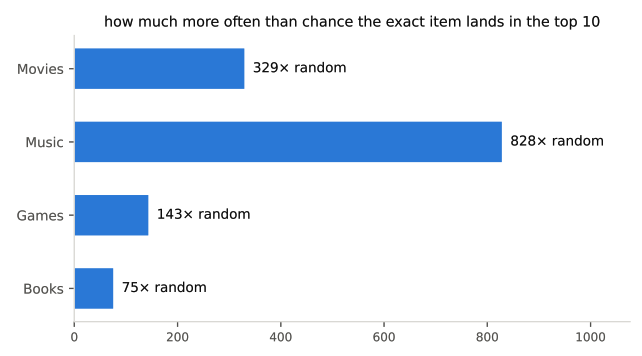
\includegraphics[width=0.8\textwidth]{figures/image32}
  \caption{HR@10 performance of FL-PRADO over different target domains.}
  \label{fig:ch5_f1}
\end{figure}

Figure 5.2 shows the cumulative distribution of the true item’s rank. The x-axis is a log-scale representation of the rank assigned to the correct item among different items in the candidate set. The Y-axis shows the cumulative percentage of queries for which the correct item appears at/ above rank. The steeper rising curve of FL-PRADO indicates that the correct item is consistently ranked near the top. The dashed gray curve shows the random recommender performance.

\begin{figure}[htbp]
  \centering
  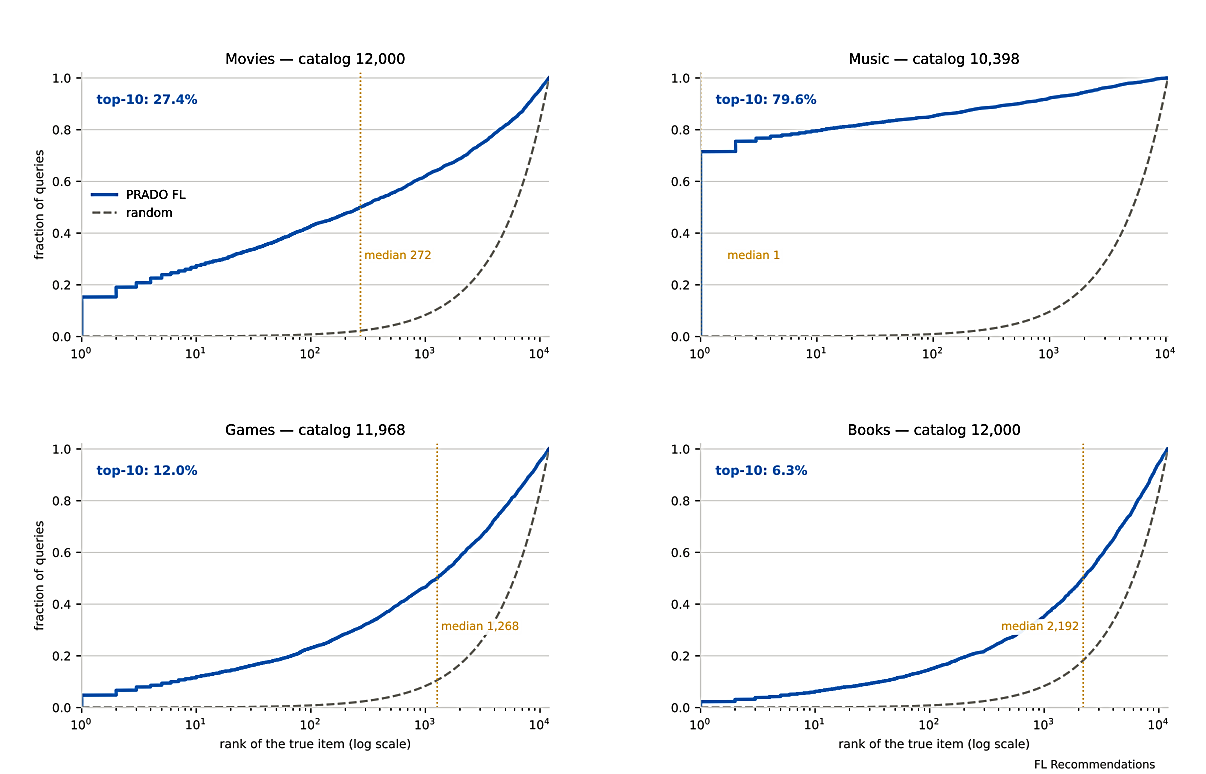
\includegraphics[width=0.8\textwidth]{figures/image33}
  \caption{Cumulative distribution of the true item's rank.}
  \label{fig:ch5_f2}
\end{figure}

\subsection{FL-PRADO (V1 vs. V2)}
Section 4.3 describes the two different implementations of FL-PRADO as V1 and V2 (embeddings + document queries, same MLServer FedAvg weights $\cdot$ 128-d penultimate embedding $\cdot$ query = held-out half of the item's chunks $\cdot$ 3-view ensemble scorer). This section describes the performance difference between these two versions. Table 5.3 demonstrates the enhanced retrieval pipeline (V2) results. V1 and V2 receive the same federated model weights. HR@10 measures the percentage of those queries for which the correct item is listed among the top 10 retrieved results. Out of four target domains, for Movies, V2 achieves a 27.4\% hit ratio, which is a 74X improvement over V1 and a 23X improvement over BERT. This indicates V2 captures movie semantics much more effectively. For music, it receives the highest hit ratio. For Games and Books, the HR@10 is lower, but there is still improvement over V1 and BERT. Median Rank indicates the position of the correct item in the ranking list, lower values are better. From Table 5.3, median rank improves for Movies in V2 drastically as compared to V1 and BERT. For music, it is 1. This indicates the correct song is top-ranked for more than half of all the queries. There is substantial improvement in Median rank for the Games and Books domains too.

Mean Reciprocal Rank (MRR) gives the average of the reciprocal of its rank. Larger values indicate better ranking. For all four domains, there is improvement in MRR (> 75X on average).

\begin{table}[htbp]
  \centering
  \caption{Headline Retrieval Results}
  \label{tab:ch5_t3}
  \begin{tabular}{|c|c|c|c|c|c|c|c|}
    \hline
    & \multicolumn{4}{c|}{HR@10} & \multicolumn{3}{c|}{Median Rank} \\
    \cline{2-8}
    Domain & v2 & v1 & BERT & Random & v2 & v1 & Random \\
    \hline
    Movies & 27.4\% & 0.37\% & 1.17\% & 0.083\% & 272 & 4,376 & 6,000 \\
    \hline
    Music & 79.6\% & 11.90\% & 6.10\% & 0.096\% & 1 & 1,204 & 5,200 \\
    \hline
    Games & 12.0\% & 0.37\% & 0.67\% & 0.084\% & 1,268 & 4,244 & 5,984 \\
    \hline
    Books B & 6.3\% & 0.57\% & 2.20\% & 0.083\% & 2,192 & 4,600 & 6,000 \\
    \hline
    & \multicolumn{4}{c|}{MRR} & \multicolumn{3}{c|}{NDCG@10} \\
    \cline{2-8}
    Domain & v2 & v1 & BERT & Random & v2 & v1 & BERT \\
    \hline
    Movies & 19.5\% & 0.23\% & 0.57\% & 0.083\% & 20.9\% & 0.17\% & 0.56\% \\
    \hline
    Music & 74.7\% & 8.12\% & 3.33\% & 0.095\% & 75.7\% & 8.68\% & 3.62\% \\
    \hline
    Games & 7.3\% & 0.23\% & 0.38\% & 0.083\% & 8.0\% & 0.17\% & 0.29\% \\
    \hline
    Books B & 3.7\% & 0.40\% & 1.11\% & 0.083\% & 4.0\% & 0.34\% & 1.10\% \\
    \hline
  \end{tabular}
\end{table}

NDCG@10 (Normalized Discounted Cumulative Gain) rewards correct items appearing at the

top 10 results. For Movies, V2 achieves 20.9\%, which is substantially greater than V1 and BERT.

For Music, it is highest and lower for Games and Books.

\begin{figure}[htbp]
  \centering
  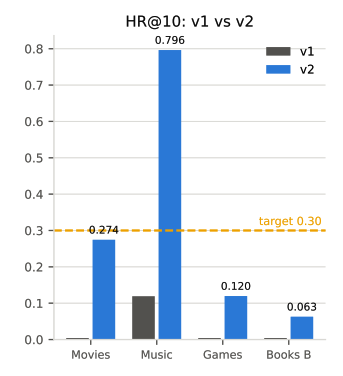
\includegraphics[width=0.8\textwidth]{figures/image34}
  \caption{Hit rate comparison between V1 and V2}
  \label{fig:ch5_f3}
\end{figure}

Figure  5.3 demonstrated the Hit rate comparison between two versions of the proposed model.

\subsection{CDR Frameworks Evaluation}
In the field of cross-domain recommendation (CDR), researchers have explored a number of representative models, each using a different learning paradigm to transfer knowledge across domains. Since there aren't any directly comparable baseline approaches, we selected four popular and typical models: EMCDR \cite{ref86}, CDFLM \cite{ref87}, ANR \cite{ref88}, and MFPCDR \cite{ref89}.

The EMCDR framework uses a multilayer perceptron (MLP) to learn how to translate nonlinearly between the source and target domains. This helps improve cross-domain recommendation effectiveness by aligning user and item embeddings. The ANR model, in contrast, employs an attention-based process within an aspect-oriented framework. The model is first trained on the target domain. Then, reviews from the source domain that are related to the target domain are added to improve the accuracy of the recommendations \cite{ref87} .

The CDLFM approach employs latent feature mapping to find patterns of user behavior in various fields. It employs a domain-based gradient boosting tree to transfer knowledge across domains to aid the cold-start problem by using some hidden user attributes \cite{ref88}.

The MFPCDR framework builds on this concept in a federated learning environment, integrating meta-learning and attention techniques to provide customized recommendations while preserving privacy \cite{ref89}.

To enable a comprehensive comparison between these methods, it is evident that they differ significantly in application aspects, privacy principles, and design procedures. The EMCDR model does not have any privacy-saving mechanism that cuts across the Books and Movies spheres. It applies a multilayer perceptron. The Books and Movies domains also apply to CDLFM, which maps latent features with a gradient boosting tree, but it is not privacy-preserving. The ANR model is applicable to both the Movies and CDs domains and has an attention mechanism, which enhances recommendation quality. It, however, does not consider privacy. MFPCDR, conversely, incorporates attention and transfer learning into a federated learning system, thus protecting user privacy in the Books and Movies fields.  The MFCDR with the PRADO(FL-PRADO) model builds on these ideas by combining a projected attention network with transfer learning to enable privacy-preserving knowledge transfer between the Emotion and different domains (Books, Movies, Music, and Games). This makes it a more secure and flexible way to recommend things across domains.

The original centralized EMCDR, ANR, and CDFLM models were adapted into the federated learning environment. By comparing all models under the federated settings, we ensure a fair and consistent comparison between different models, which eliminates bias caused by different training architectures.

Dataset across CDR: Different source domains across the same target domain are used for comparative analysis to strengthen the concept of emotion as a base for personalized recommendation.

The comparison is performed across the following source-domain to target-domain pairs: EMCDR (Books, Movies), ANR (Music, Movies), CDFLM (Ratings, Movies), MFPCDR (Books, Movies), and FL-PRADO (Emotions, Movies).

The models tested and shown in Table 5.4 are ranked in terms of HR@10, HR@20, NDCG@10, NDCG@20, and MRR.

Table 5.4 and the plot in Figure 5.4 benchmark the recommendation performance of the proposed FL-PRADO model against the best baseline models. FL-PRADO achieves the highest HR@10 of 27.4\%, outperforming MFPCDR (17.21\%) by 10.19 percentage points (59.2\%) and FL-EMCDR (15.35\%) by 12.05 percentage points (78.5\%). Similarly, FL-PRADO attains the best HR@20 of 31.6\%, exceeding MFPCDR (21.35\%) by 10.25 percentage points (48.0\%) and FL-EMCDR (21.61\%) by 9.99 percentage points (46.2\%).

\begin{longtable}{|p{2.5cm}|p{2cm}|p{2cm}|p{2cm}|p{2cm}|p{2cm}|}
\caption{Analysis of Ranking Quality for different models}
\label{tab:ch5_t4} \\
\hline
Model & HR@10 & HR@20 & NDCG@10 & NDCG@20 & MRR \\
\hline
\endfirsthead
\hline
Model & HR@10 & HR@20 & NDCG@10 & NDCG@20 & MRR \\
\hline
\endhead
\hline
\endfoot
EMCDR* & 9.10\% & 14.46\% & 4.97\% & 6.32\% & 4.19\% \\
\hline
ANR* & 4.54\% & 6.87\% & 3.65\% & 5.97\% & 3.91\% \\
\hline
CDFLM* & 8.94\% & 17.42\% & 5.44\% & 6.18\% & 4.22\% \\
\hline
FL-EMCDR & 15.35\% & 21.61\% & 9.73\% & 12.05\% & 8.47\% \\
\hline
FL-ANR & 7.31\% & 12.96\% & 6.39\% & 9.80\% & 6.51\% \\
\hline
FL-CDFLM & 7.72\% & 13.04\% & 3.37\% & 4.71\% & 3.18\% \\
\hline
MFPCDR & 17.21\% & 21.35\% & 12.33\% & 13.14\% & 10.13\% \\
\hline
FL-PRADO & 27.4\% & 31.6\% & 20.9\% & 21.8\% & 19.5\% \\
\hline
\multicolumn{6}{|l|}{* Indicates a non-FL environment for the model training} \\
\hline
\end{longtable}

\begin{figure}[htbp]
  \centering
  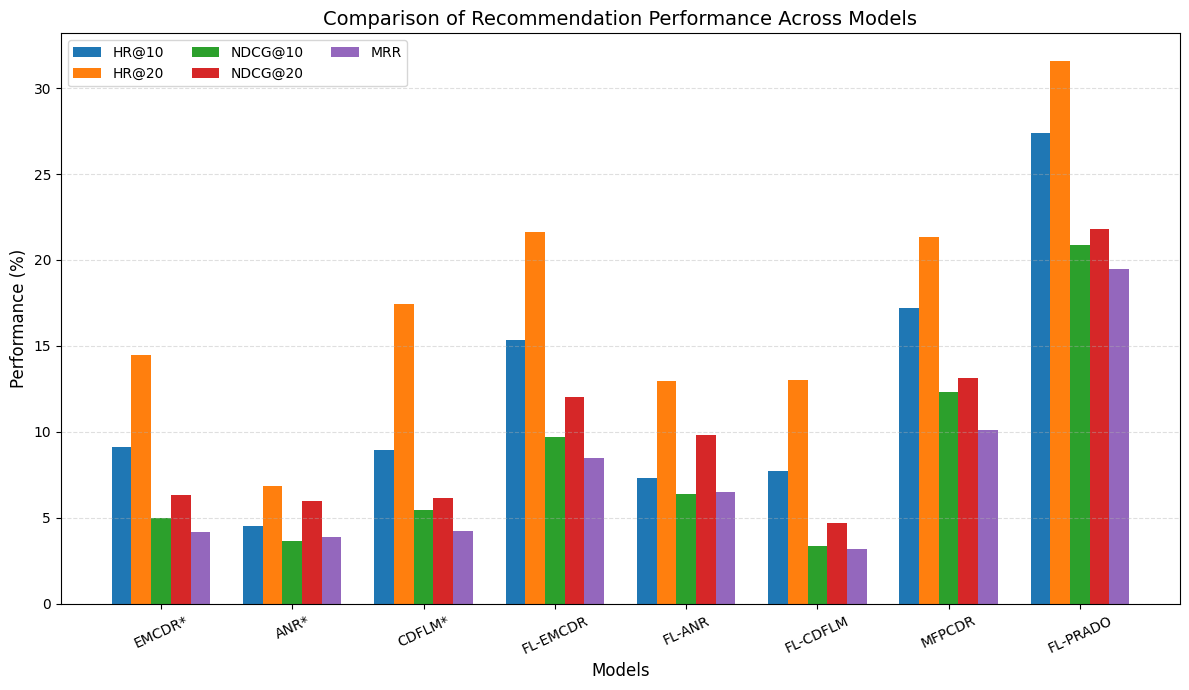
\includegraphics[width=0.8\textwidth]{figures/image35}
  \caption{Recommendation Performance Comparison}
  \label{fig:ch5_f4}
\end{figure}

The NDCG@10 of FL-PRADO is 20.9\%, an improvement of 69.5\% over MFPCDR (12.33\%) and 114.8\% over FL-EMCDR (9.73\%). Likewise, NDCG@20 reaches 21.8\%, surpassing MFPCDR (13.14\%) by 65.9\% and FL-EMCDR (12.05\%) by 80.9\%.

In terms of MRR, FL-PRADO achieves 19.5\%, improving upon MFPCDR (10.13\%) by 92.5\% and FL-EMCDR (8.47\%) by 130.2\%. The results show that FL-PRADO achieves the best retrieval accuracy and ranking performance compared to other state-of-the-art non-federated and federated recommendation models.

In general, the experimental results confirm that the FL-PRADO(V2) model gives the best top-K recommendations and the best ranking quality among all the models evaluated. The steady increase in HR, NDCG, and MRR scores confirms the success of incorporating federated representation learning based on PRADO with the proposed cross-domain recommendation framework for preserving privacy while also achieving better recommendation performance.

\section{Summary}
This chapter conducted a detailed review of the proposed MFCDR concept across various recommendation areas. The proposed FL-PRADO model achieved the best performance in terms of HR@10, HR@20, NDCG, and MRR. The highest Hit Rate (HR@10) of the proposed model, i.e., 79.6\%, is recorded for song recommendation (Music), along with MRR 74.7\%, median rank 1, and NDGC@10 is 75.7. Comparative experiments shown in Figure 5.4 demonstrate that the proposed FL-PRADO model consistently outperformed the centralized, federated, and state-of-the-art recommendation models. The results demonstrate the effectiveness of federated learning combined with PRADO in providing privacy-preserving cross-domain recommendations, with higher recommendation accuracy, better ranking quality, scalability, and user privacy. This chapter meets Objective 4.


\chapter{Summary and Conclusions}
The summary and main findings along with future scope is presented in this chapter. This provides the brief overview of research work conducted.

\section{Summary}
The first chapter introduces recommendation systems and clarifies the need for Federated learning in personalized recommendations. It also discusses the classification of federated recommendation systems. Chapter 2 provides the literature review of the techniques available regarding recommendations and federated recommendation system. Also, it examines the federated cross-domain recommendation system. It presents the research work goals.

Chapter 3 explains a federated, emotion-driven, sentiment analysis model aimed at edge devices to trade off privacy, scalability and performance. The PRADO (Projected Attention Network) used in the work is implemented in a federated learning (FL) setting to overcome the shortcomings of NLP models. PRADO generates small, dynamically acquired embeddings based on the projection mechanism and convolution and attention-based layers, which can be used effectively to classify long texts with minimum memory consumption. The federated setup combines local predictions through weighted FedAvg, enabling decentralized learning while protecting user data.

Chapter 4 introduces a Multi-objective Modular Federated Cross-Domain Recommendation (MFCDR) framework.  This combines emotion recognition with personalized recommendation while maintaining privacy through Federated Learning (FL). Traditional recommendation systems mainly depend on collaborative filtering or content-based methods, but this work focuses on emotions derived from user reviews, using the GoEmotions dataset as the source domain and different datasets like Movies, Music, Books, and Games as the target domains. To address heterogeneity and synchronization delays in FL, a weighted FedAvg aggregation strategy is proposed that collects client updates only after a threshold is reached, thereby enhancing scalability and stability. The emotion embeddings produced by PRADO are also used at the recommendation layer, enabling cross-domain recommendations that effectively handle sparse data, noisy reviews, and cold-start issues.

In Chapter 5, the evaluation of the proposed model occurs in three phases. In the first phase, the model is tested for its ability to predict emotions across different target domains, such as books, music, movies, and games. Two models are trained on the GoEmotions dataset, PRADO and BERT, namely FL-PRADO and FL-BERT, using the experimental setup in Section 3.3. The second phase of evaluation compares these two models exclusively on different datasets. In addition, two versions of FL-PRADO are implemented, V1 and V2, as described in Section 3.4. The comparison among these two versions and BERT is performed on various metrics. The third phase of evaluation compares the proposed model with baseline recommenders and their FL frameworks.

The proposed FL-PRADO model achieved the best performance in terms of HR@10, HR@20, NDCG, and MRR compared to centralized and federated recommendation models as well as the best-performing state-of-the-art models. Comparative experiments showed that the proposed FL-PRADO model consistently outperformed centralized, federated, and state-of-the-art recommendation models on HR@10, HR@20, NDCG, and MRR. The results demonstrate the effectiveness of federated learning combined with PRADO in providing privacy-preserving cross-domain recommendations, with higher recommendation accuracy, better ranking quality, scalability, and user privacy.

\section{Conclusions}
The following conclusions are drawn from the investigation presented in this thesis:

\begin{enumerate}
  \item The research confirms the feasibility of cross-domain suggestions in privacy-sensitive environments based on Federated learning.
  \item The adoption of emotional embeddings in the recommendation system has improved its performance tremendously, which has been confirmed by using different baselines and SOTA models.
  \item The developed model applies knowledge transfer by extracting emotions from reviews and mapping them to the different target domains.
\end{enumerate}

\section{Future Scope}
The proposed MFCDR framework demonstrates strong potential for privacy-preserving, emotionally oriented recommendations. Several research directions can be identified. To begin with, expanding datasets to multilingual and multicultural contexts can be added to the dataset to enhance their generalizability and reduce bias. The inclusion of multimodal information, i.e., audio, video, and physiological signals, might increase the accuracy of emotion prediction, as it will have denser contextual information.



% ---- Back matter ----
\backmatter

% ---- Bibliography (1.6 References — comes before Publications) ----
\singlespacing
\renewcommand{\bibname}{References}
\bibliographystyle{plainnat}
\bibliography{references}

% ---- Publications by the candidate (1.8 — after Literature Cited) ----
%% =====================================================
%% LIST OF PUBLICATIONS BY THE CANDIDATE
%% =====================================================
\clearpage
\pubschapter

\noindent
\begin{enumerate}
\item M. S. Otari, B. S. Kumar, and M. B. Patil, ``Challenges and advancement in federated recommendation system: A comprehensive review,'' in \emph{Accelerating Discoveries in Data Science and Artificial Intelligence I}, Springer Proceedings in Mathematics \& Statistics, vol. 421, F. M. Lin, A. Patel, N. Kesswani, and B. Sambana, Eds. Cham: Springer Nature Switzerland, 2024, pp. 225--234. doi: 10.1007/978-3-031-51167-7\_22.

\item M. S. Otari, B. S. Kumar, and M. B. Patil, ``Security, privacy, and communication efficiency in federated learning: Issues and perspectives,'' in \emph{Innovations in Cybersecurity and Data Science}, S. M. Basha, H. Taherdoost, and C. Zanchettin, Eds. Singapore: Springer Nature Singapore, 2024, pp. 237--247. doi: 10.1007/978-981-97-5791-6\_19.

\item M. S. Otari, D. Patil, and M. B. Patil, ``Revolutionizing emotion-driven sentiment analysis using federated learning on edge devices for superior privacy and performance,'' \emph{Nanotechnology Perceptions}, Jun. 2024. doi: 10.62441/nano-ntp.vi.1342.

\item M. S. Otari, D. Patil, and M. B. Patil, ``Modular Federated Cross-Domain Recommendation (MFCDR) System with a Projected Attention Network,'' \emph{J. Comput. Cogn. Eng.}, Oct. 2025. doi: 10.47852/bonviewJCCE52026111.

\item M. S. Otari, D. Patil, and M. B. Patil, ``Privacy-Preserving Sentiment Analysis: A Model-Level performance evaluation using Federated learning,'' \emph{IAENG International Journal of Computer Science}, under review.

\item Filed an Indian Utility Patent entitled ``Privacy-preserving federated learning system and method for emotion prediction using projected attention networks.''
\end{enumerate}

\end{document}
